\newpage
\chapter{HASIL DAN PEMBAHASAN} \label{Bab IV}

\section{Deskripsi Dataset} \label{IV.Deskripsi_dataset}
Penelitian ini menggunakan empat dataset \textit{benchmark} untuk mengevaluasi performa metode HOUM. Tiga dataset pertama, yaitu Diabetes, Haberman, dan Transfusion, mengacu pada penelitian Eroglu dan Pir (2024) \cite{Eroglu2024HOUM}. Dataset keempat, yaitu Glass5, ditambahkan untuk menguji performa HOUM pada kondisi ketidakseimbangan yang tinggi. Keempat dataset dipilih karena memiliki tingkat ketidakseimbangan kelas yang berbeda, sehingga dapat merepresentasikan variasi kompleksitas dalam penanganan data tidak seimbang. Ringkasan statistik dataset disajikan pada Tabel \ref{table:4.statistik_dataset}.

\begin{table}[H]
\centering
\caption{Statistik Dataset yang Digunakan}
\label{table:4.statistik_dataset}
\begin{tabular}{|l|c|c|c|c|c|}
\hline
\textbf{Dataset} & \textbf{Jumlah Data} & \textbf{Fitur} & \textbf{Mayoritas} & \textbf{Minoritas} & \textbf{Rasio} \\
\hline
Diabetes & 768 & 8 & 500 (65,10\%) & 268 (34,90\%) & 1:1,87 \\
\hline
Transfusion & 748 & 4 & 570 (76,20\%) & 178 (23,80\%) & 1:3,20 \\
\hline
Haberman & 306 & 3 & 225 (73,53\%) & 81 (26,47\%) & 1:2,78 \\
\hline
Glass5 & 214 & 9 & 205 (95,79\%) & 9 (4,21\%) & 1:22,78 \\
\hline
\end{tabular}
\end{table}

Dataset Pima Indians Diabetes terdiri dari 768 data pasien perempuan dengan delapan fitur numerik dan target diagnosis diabetes. Kelas mayoritas berjumlah 500 data (65,10\%), sedangkan kelas minoritas sebanyak 268 data (34,90\%), dengan rasio ketidakseimbangan sebesar 1:1,87 yang tergolong rendah. \par

Dataset Blood Transfusion Service Center berisi 748 data donor dengan empat fitur utama terkait riwayat donasi. Target klasifikasi menentukan kemungkinan donor melakukan donasi kembali. Dataset ini memiliki 570 data mayoritas (76,20\%) dan 178 data minoritas (23,80\%), dengan rasio ketidakseimbangan sebesar 1:3,20. \par

Dataset Haberman memuat 306 data pasien kanker payudara dengan tiga fitur, yaitu usia, tahun operasi, dan jumlah kelenjar getah bening positif. Target klasifikasi menunjukkan tingkat kelangsungan hidup pasien. Dataset ini memiliki 225 data mayoritas (73,53\%) dan 81 data minoritas (26,47\%), dengan rasio ketidakseimbangan sebesar 1:2,78. \par

Dataset Glass5 memuat data identifikasi jenis kaca berdasarkan komposisi kimianya yang diperoleh dari UCI \textit{Machine Learning Repository}. Dataset ini terdiri dari 214 instansi dengan sembilan fitur numerik yang mencakup indeks bias (\textit{Refractive Index}), serta kandungan unsur kimia seperti Natrium (Na), Magnesium (Mg), Aluminium (Al), Silikon (Si), Kalium (K), Kalsium (Ca), Barium (Ba), dan Besi (Fe). Target klasifikasi berupa penentuan apakah suatu sampel kaca termasuk ke dalam kelas tertentu (kelas minoritas) atau bukan (kelas mayoritas). Dataset ini memiliki 205 data mayoritas (95,79\%) dan 9 data minoritas (4,21\%), dengan rasio ketidakseimbangan sebesar 1:22,78 yang merupakan yang tertinggi di antara keempat dataset yang digunakan. Dengan hanya sembilan sampel pada kelas minoritas, dataset ini menjadi kasus ekstrem untuk menguji kemampuan HOUM dalam menangani data dengan kelangkaan sampel minoritas yang tinggi. \par

Distribusi kelas masing-masing dataset divisualisasikan pada Gambar \ref{fig:4.distribusi_kelas} untuk memperjelas perbandingan jumlah sampel antar kelas.

\begin{figure}[H]
    \centering
    \begin{subfigure}[b]{0.47\textwidth}
        \centering
        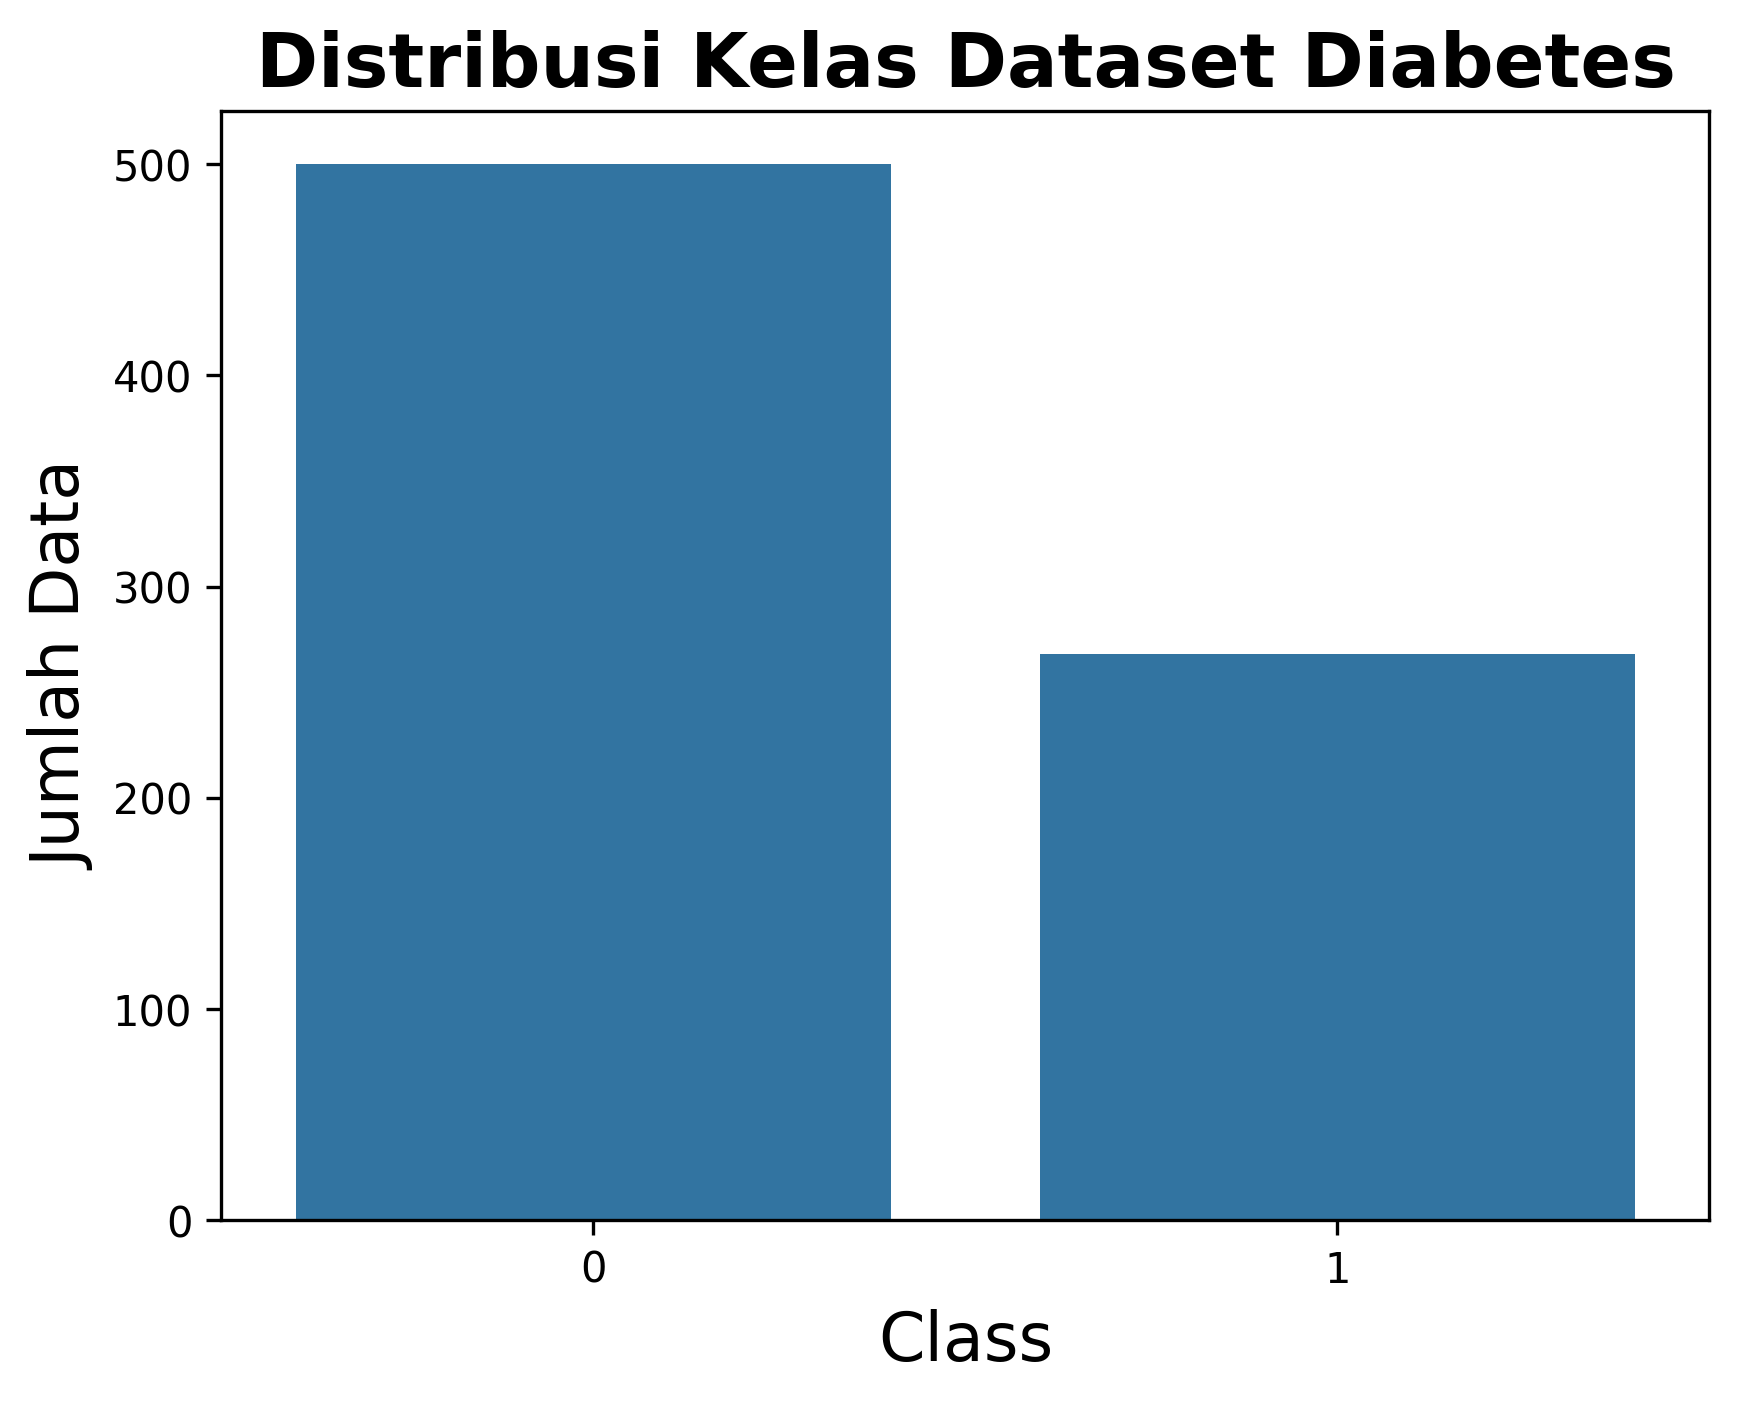
\includegraphics[width=\textwidth]{figure/distribusi_kelas_diabetes.png}
        \caption{Diabetes}
        \label{fig:4.dist_diabetes}
    \end{subfigure}
    \hfill
    \begin{subfigure}[b]{0.47\textwidth}
        \centering
        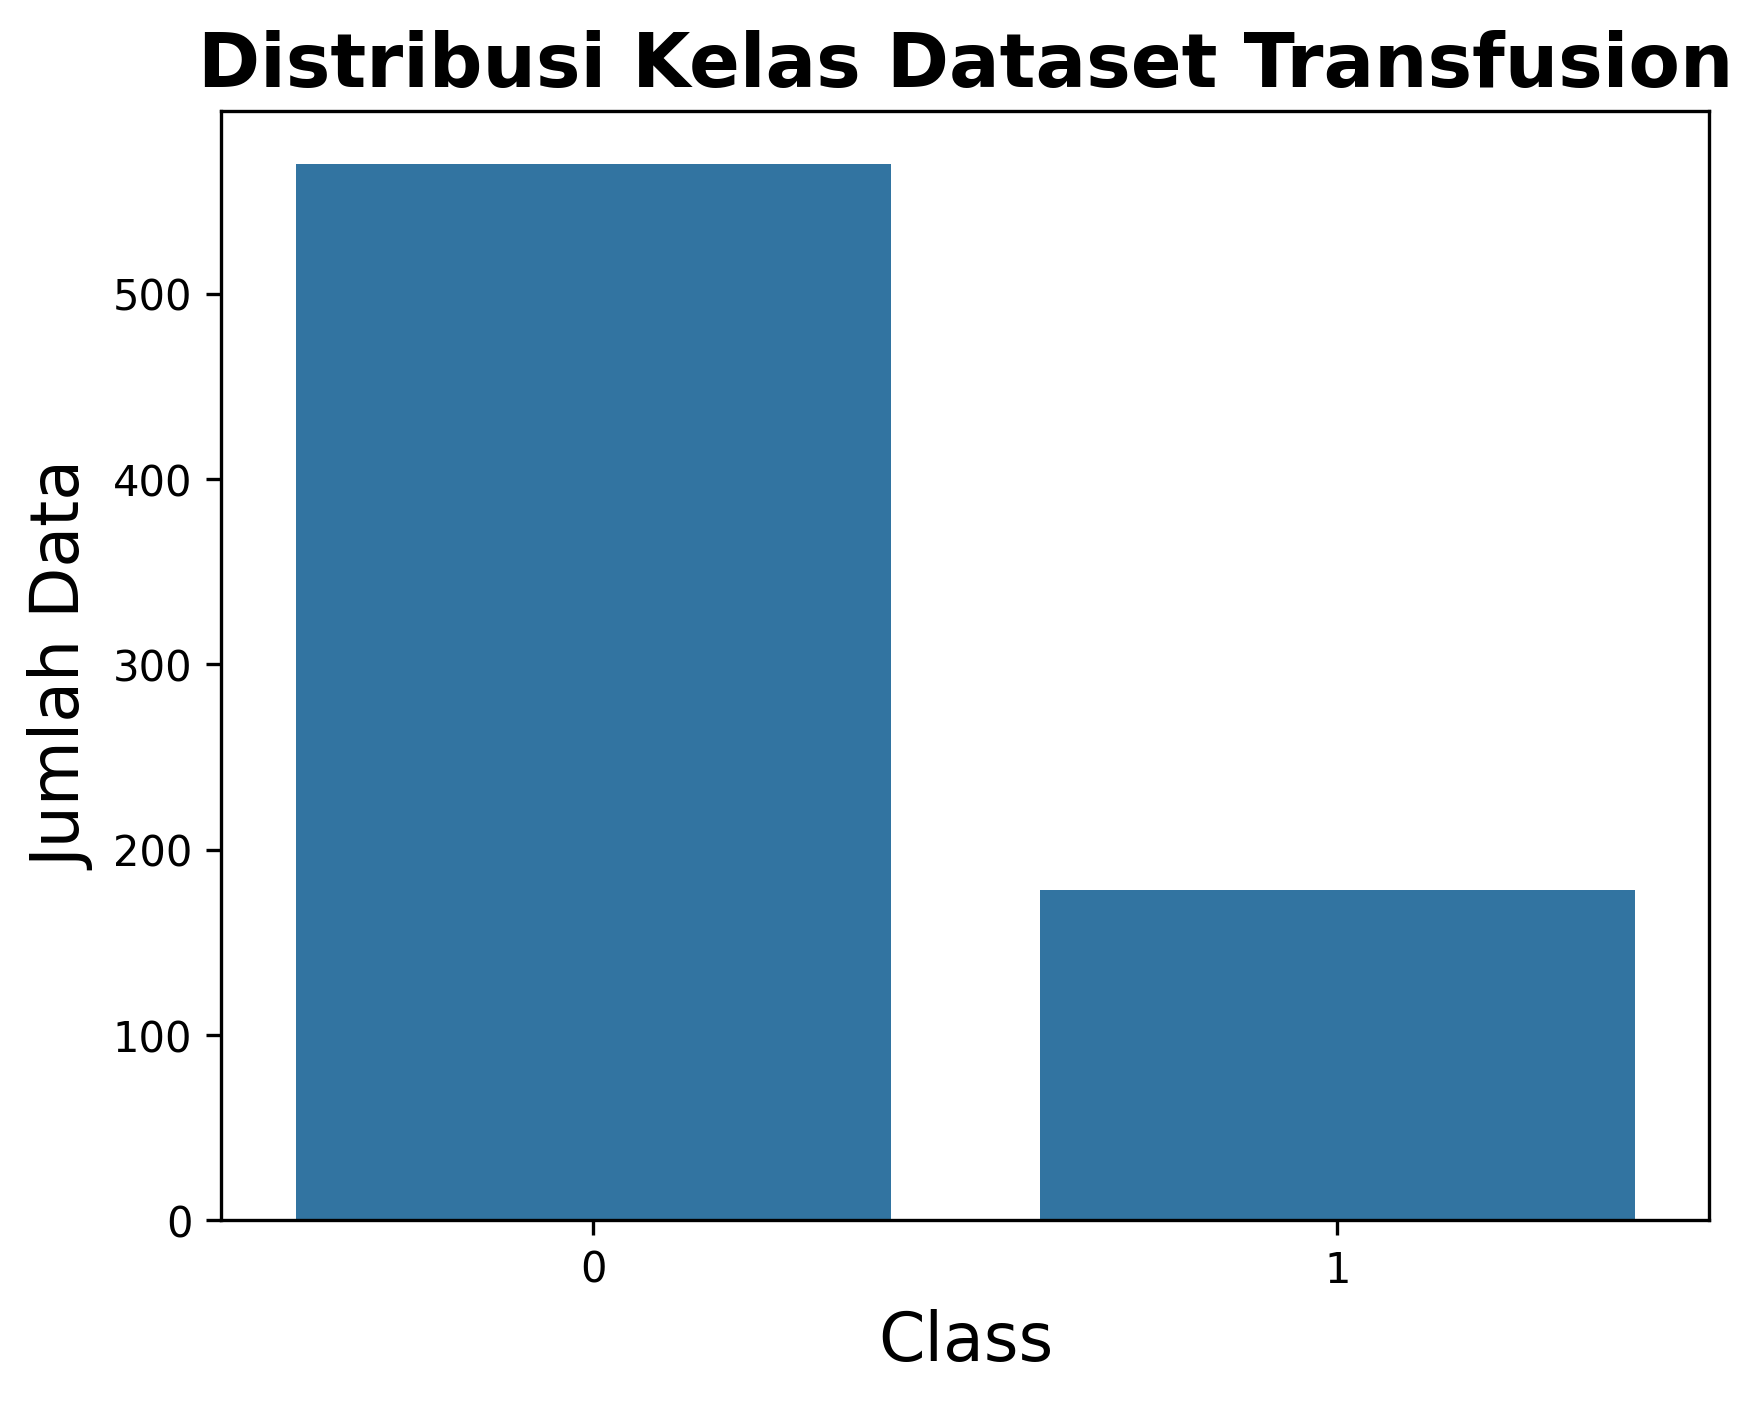
\includegraphics[width=\textwidth]{figure/distribusi_kelas_transfusion.png}
        \caption{Transfusion}
        \label{fig:4.dist_transfusion}
    \end{subfigure}

    \vspace{0.5em}

    \begin{subfigure}[b]{0.47\textwidth}
        \centering
        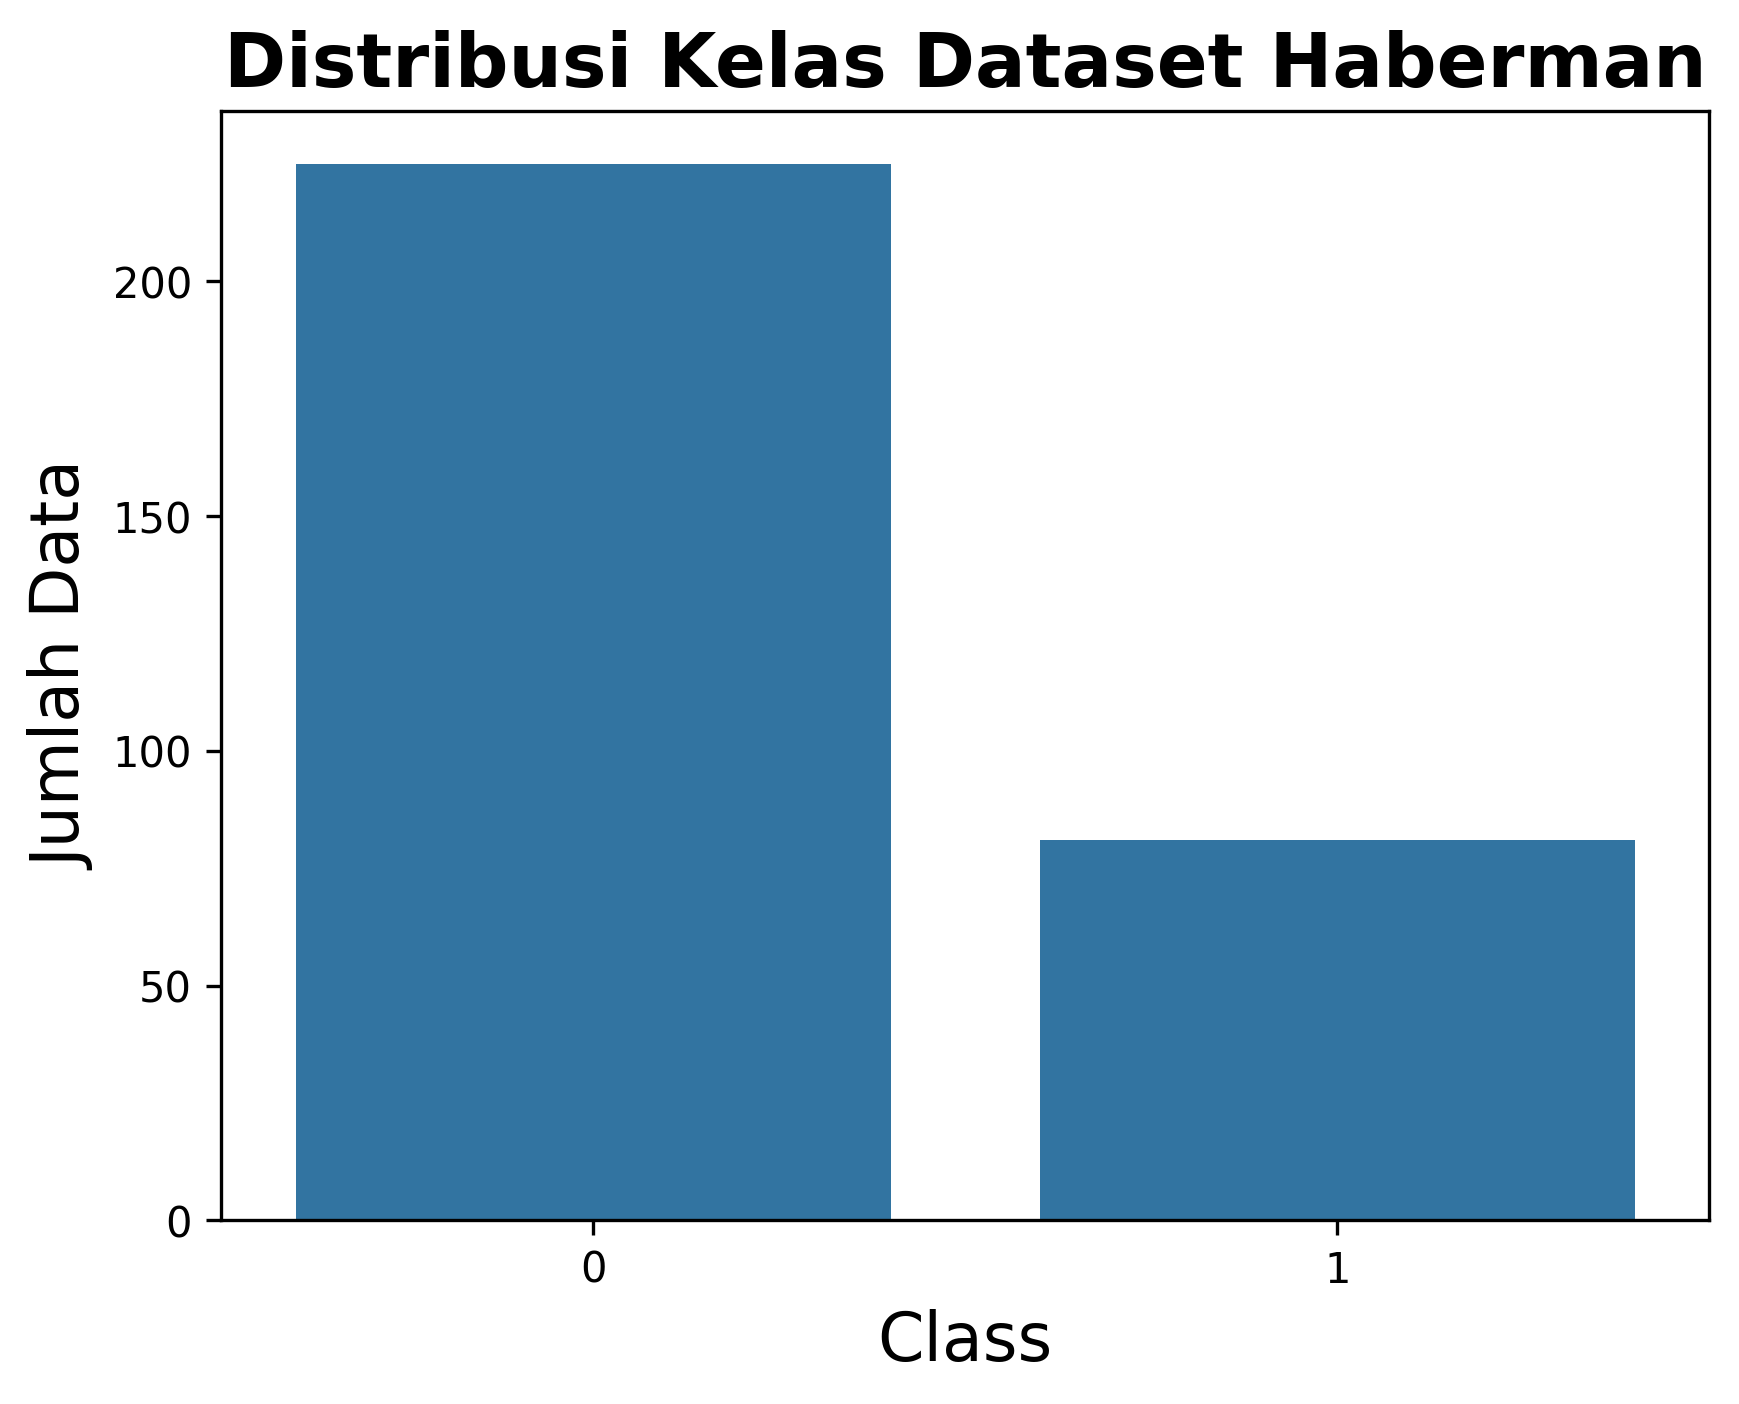
\includegraphics[width=\textwidth]{figure/distribusi_kelas_haberman.png}
        \caption{Haberman}
        \label{fig:4.dist_haberman}
    \end{subfigure}
    \hfill
    \begin{subfigure}[b]{0.47\textwidth}
        \centering
        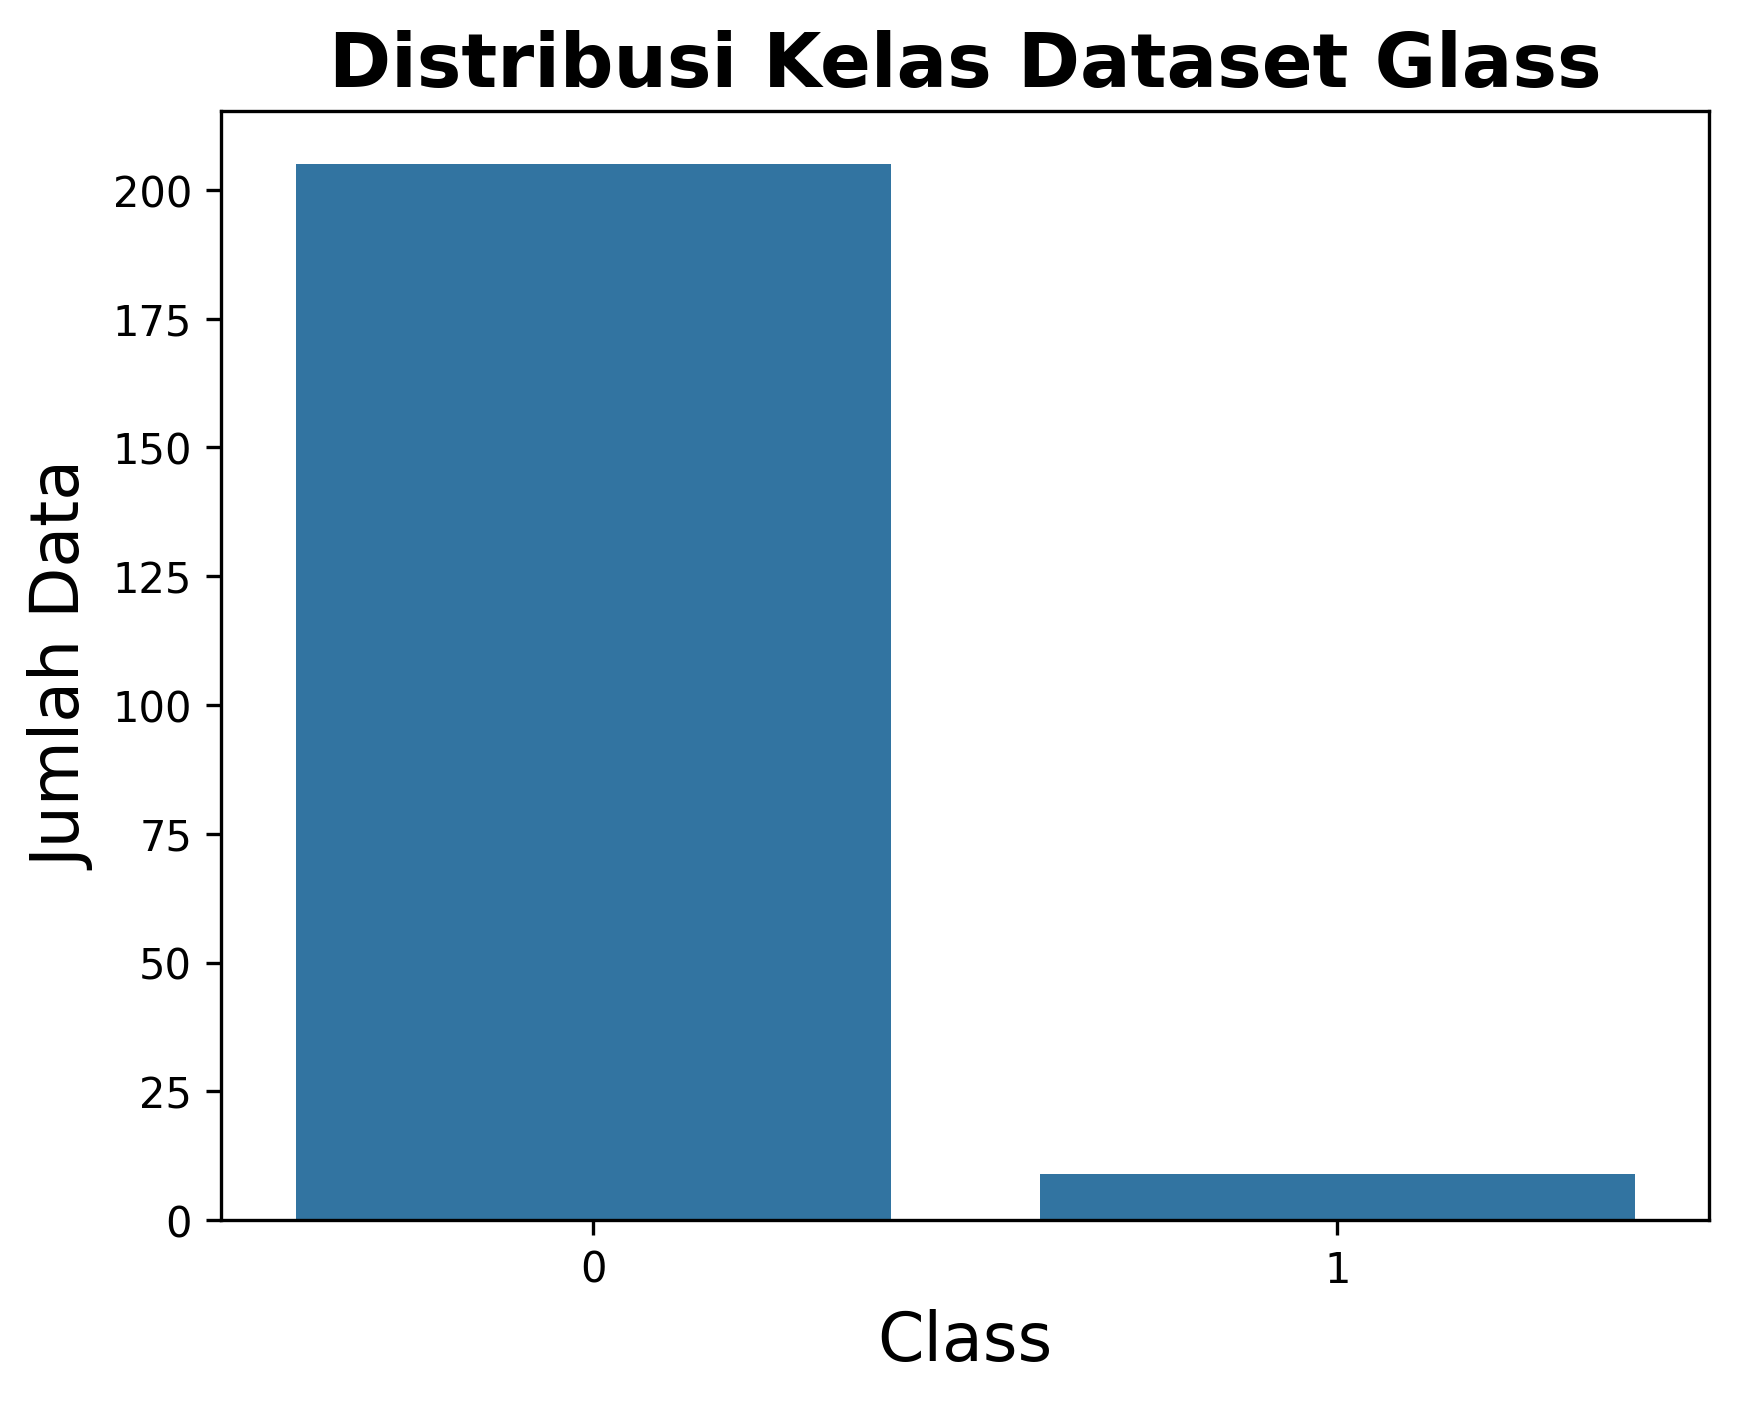
\includegraphics[width=\textwidth]{figure/distribusi_kelas_glass.png}
        \caption{Glass5}
        \label{fig:4.dist_glass}
    \end{subfigure}
    \caption{Distribusi Kelas pada Masing-Masing Dataset}
    \label{fig:4.distribusi_kelas}
\end{figure}

Berdasarkan Tabel \ref{table:4.statistik_dataset} dan Gambar \ref{fig:4.distribusi_kelas}, seluruh dataset menunjukkan kondisi tidak seimbang dengan tingkat yang bervariasi. Dataset Diabetes memiliki tingkat \textit{imbalance} rendah, Haberman berada pada tingkat menengah, Transfusion menunjukkan ketidakseimbangan yang lebih tinggi, sedangkan Glass5 merepresentasikan kasus ketidakseimbangan ekstrem dengan rasio 1:22,78 dan hanya sembilan sampel pada kelas minoritas. \par

Selain itu, jumlah fitur pada setiap dataset berbeda, yaitu delapan fitur pada Diabetes, empat pada Transfusion, tiga pada Haberman, dan sembilan pada Glass5. Dataset dengan jumlah fitur yang lebih sedikit berpotensi mengalami \textit{overlap} antar kelas, sehingga meningkatkan kesulitan dalam proses klasifikasi.
\section{Hasil Penelitian} \label{IV.Hasil_penelitian}
Bagian ini menyajikan hasil eksperimen yang diperoleh dari penerapan metode HOUM pada keempat dataset. Penyajian dimulai dari hasil klasifikasi pada data yang belum diseimbangkan (\textit{baseline}) sebagai acuan perbandingan, kemudian dilanjutkan dengan hasil setelah penerapan metode HOUM dengan berbagai konfigurasi.

\subsection{Hasil Klasifikasi pada Data Tidak Seimbang (\textit{Baseline})} \label{IV.Baseline}
Sebelum menerapkan metode HOUM, klasifikasi terlebih dahulu dilakukan pada data \textit{training} yang masih dalam kondisi tidak seimbang (\textit{imbalanced}) untuk memperoleh hasil \textit{baseline}. Hasil \textit{baseline} ini berfungsi sebagai titik acuan untuk mengukur seberapa besar kontribusi metode HOUM dalam meningkatkan performa klasifikasi. Model \textit{Random Forest} dilatih menggunakan data \textit{training} asli tanpa penyeimbangan, kemudian diuji pada data \textit{testing} yang telah disisihkan sejak awal. Hasil metrik evaluasi \textit{baseline} untuk keempat dataset ditunjukkan pada Tabel \ref{table:4.baseline}. \par

\begin{table}[H]
\centering
\caption{Hasil Klasifikasi \textit{Baseline} pada Data Tidak Seimbang}
\label{table:4.baseline}
\begin{tabular}{|l|c|c|c|c|}
\hline
\textbf{Dataset} & \textbf{ROC-AUC} & \textbf{\textit{Recall}} & \textbf{\textit{Precision}} & \textbf{G-Mean} \\
\hline
Diabetes & 0,8194 & 0,6111 & 0,6471 & 0,7079 \\
\hline
Transfusion & 0,7523 & 0,4167 & 0,5000 & 0,6015 \\
\hline
Haberman & 0,5557 & 0,1250 & 0,2000 & 0,3213 \\
\hline
Glass5 & 0,9878 & 0,5000 & 1,0000 & 0,7071 \\
\hline
\end{tabular}
\end{table}

Kurva ROC untuk masing-masing dataset pada kondisi \textit{baseline} divisualisasikan pada Gambar \ref{fig:4.roc_baseline} untuk menggambarkan kemampuan diskriminatif model secara visual.

\begin{figure}[H]
    \centering
    \begin{subfigure}[b]{0.47\textwidth}
        \centering
        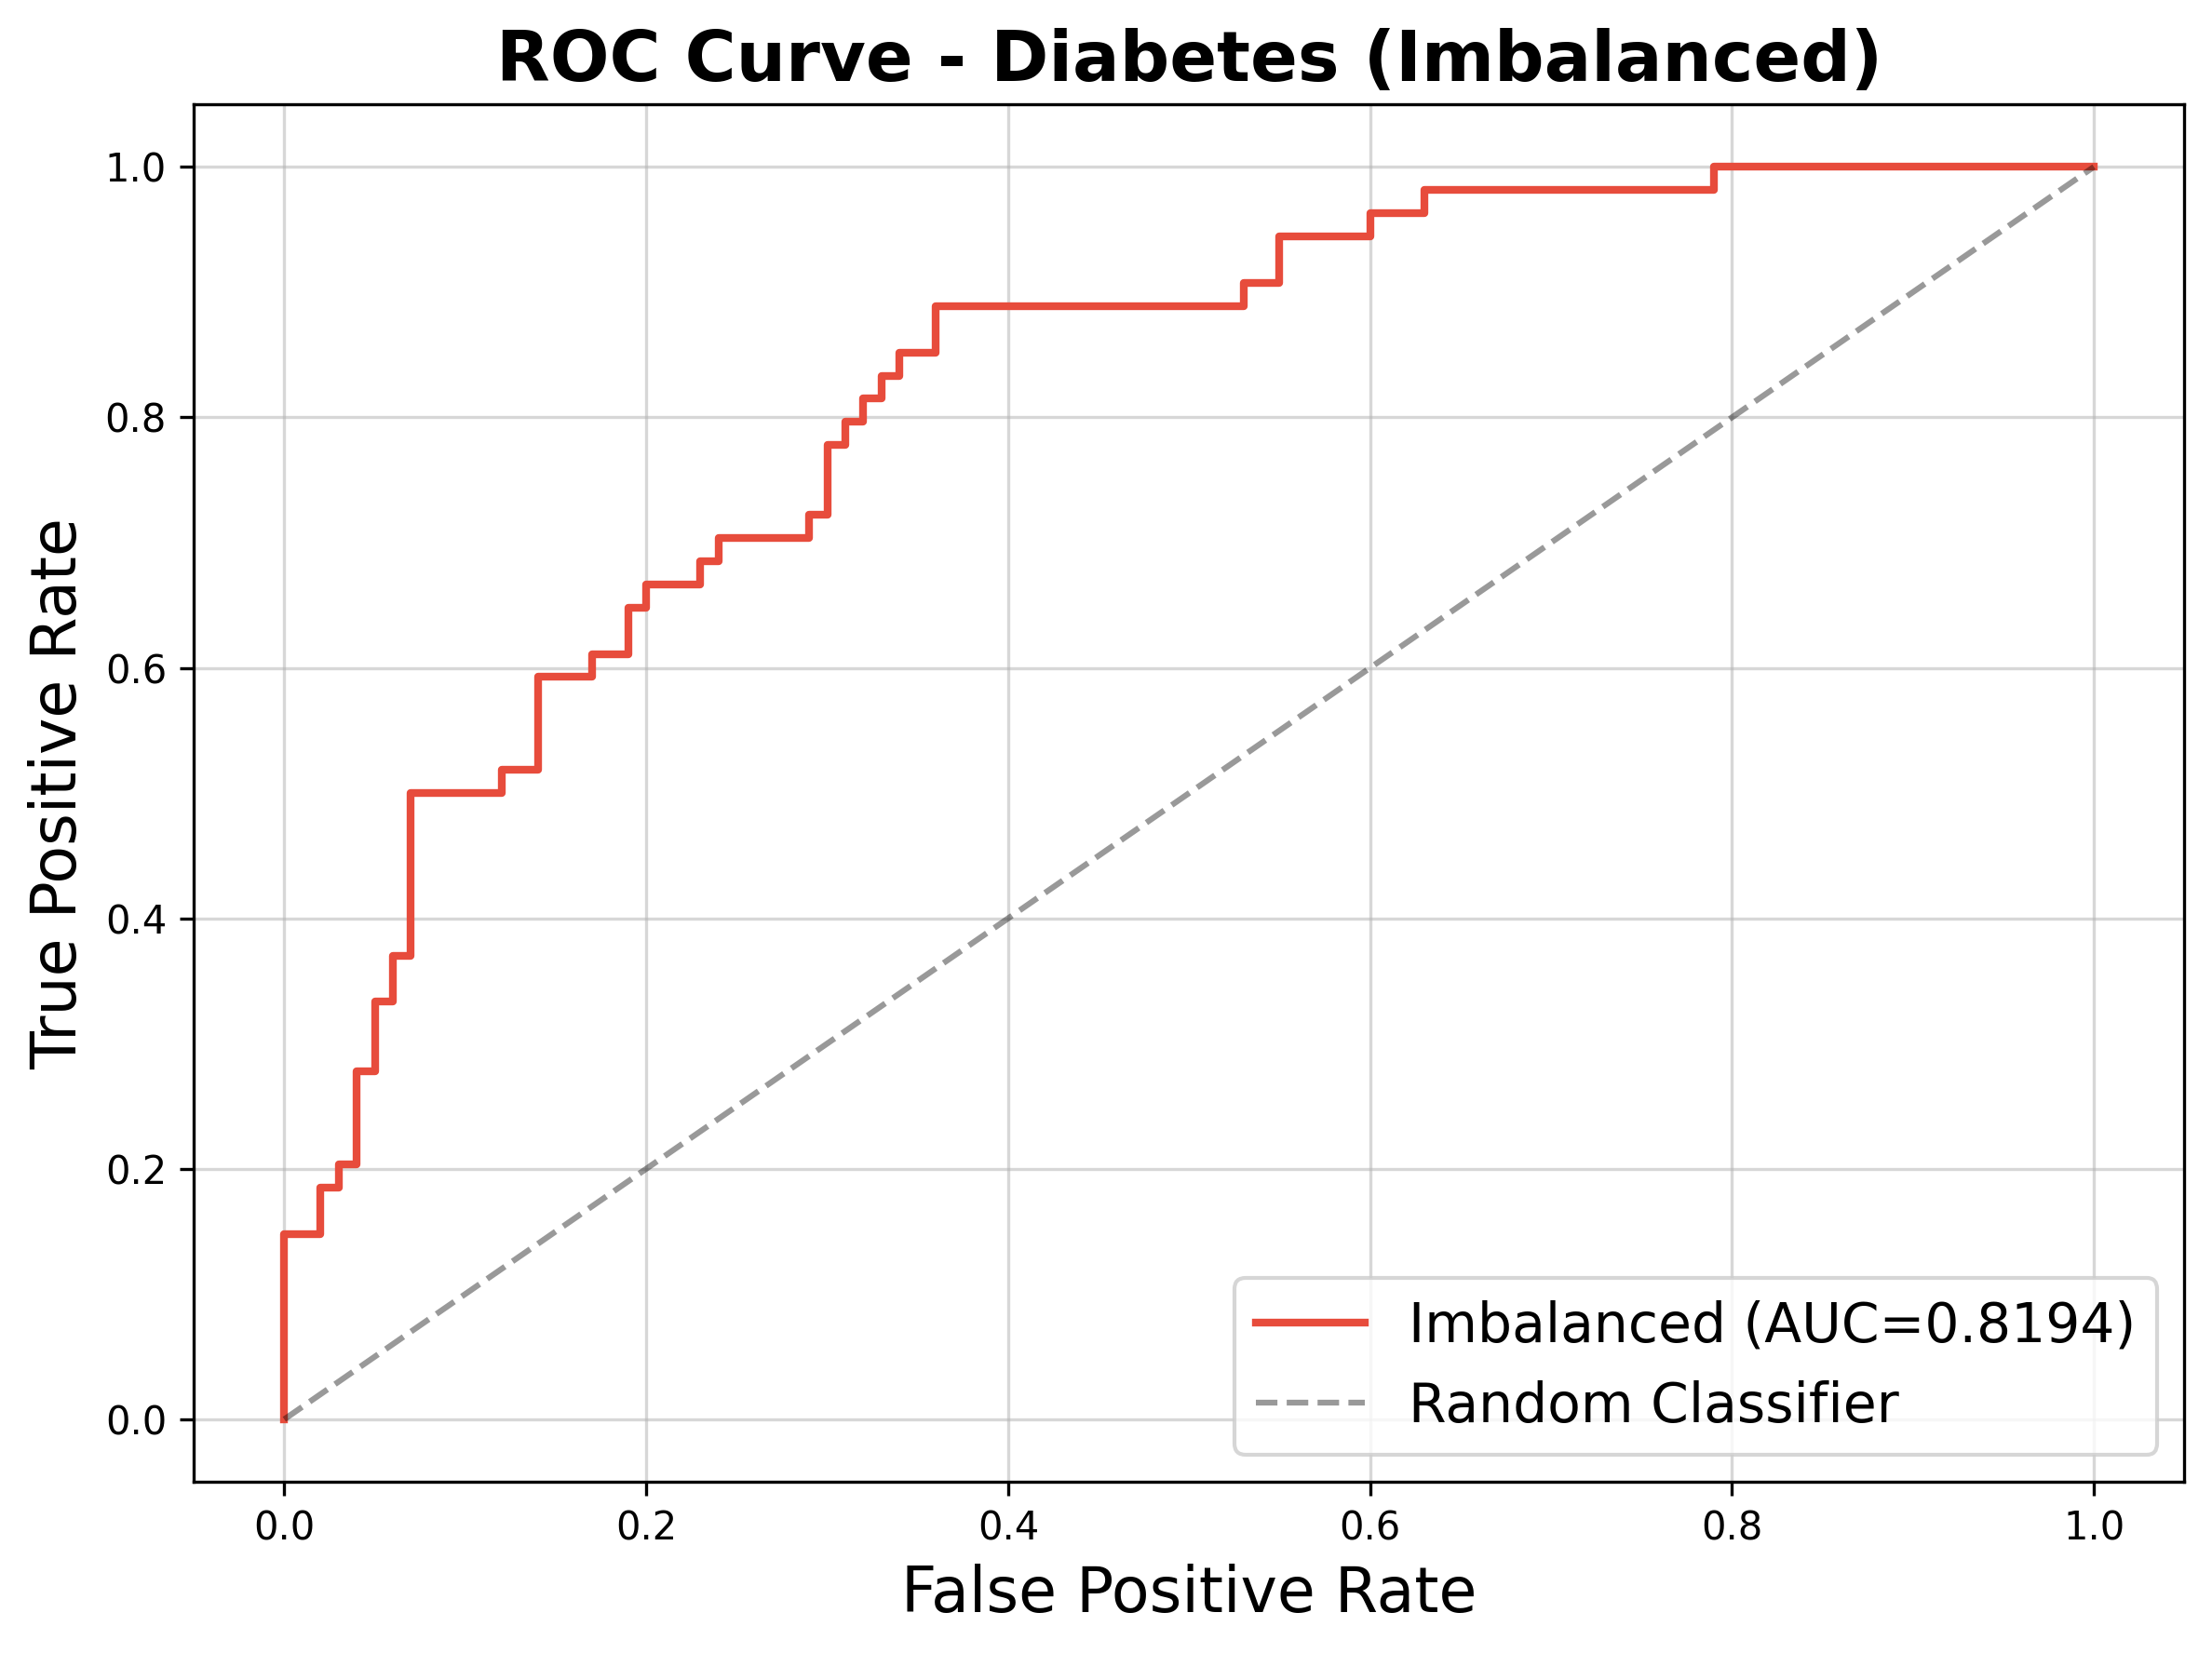
\includegraphics[width=\textwidth]{figure/roc_imbalanced_baseline_diabetes.png}
        \caption{Diabetes}
        \label{fig:4.roc_baseline_diabetes}
    \end{subfigure}
    \hfill
    \begin{subfigure}[b]{0.47\textwidth}
        \centering
        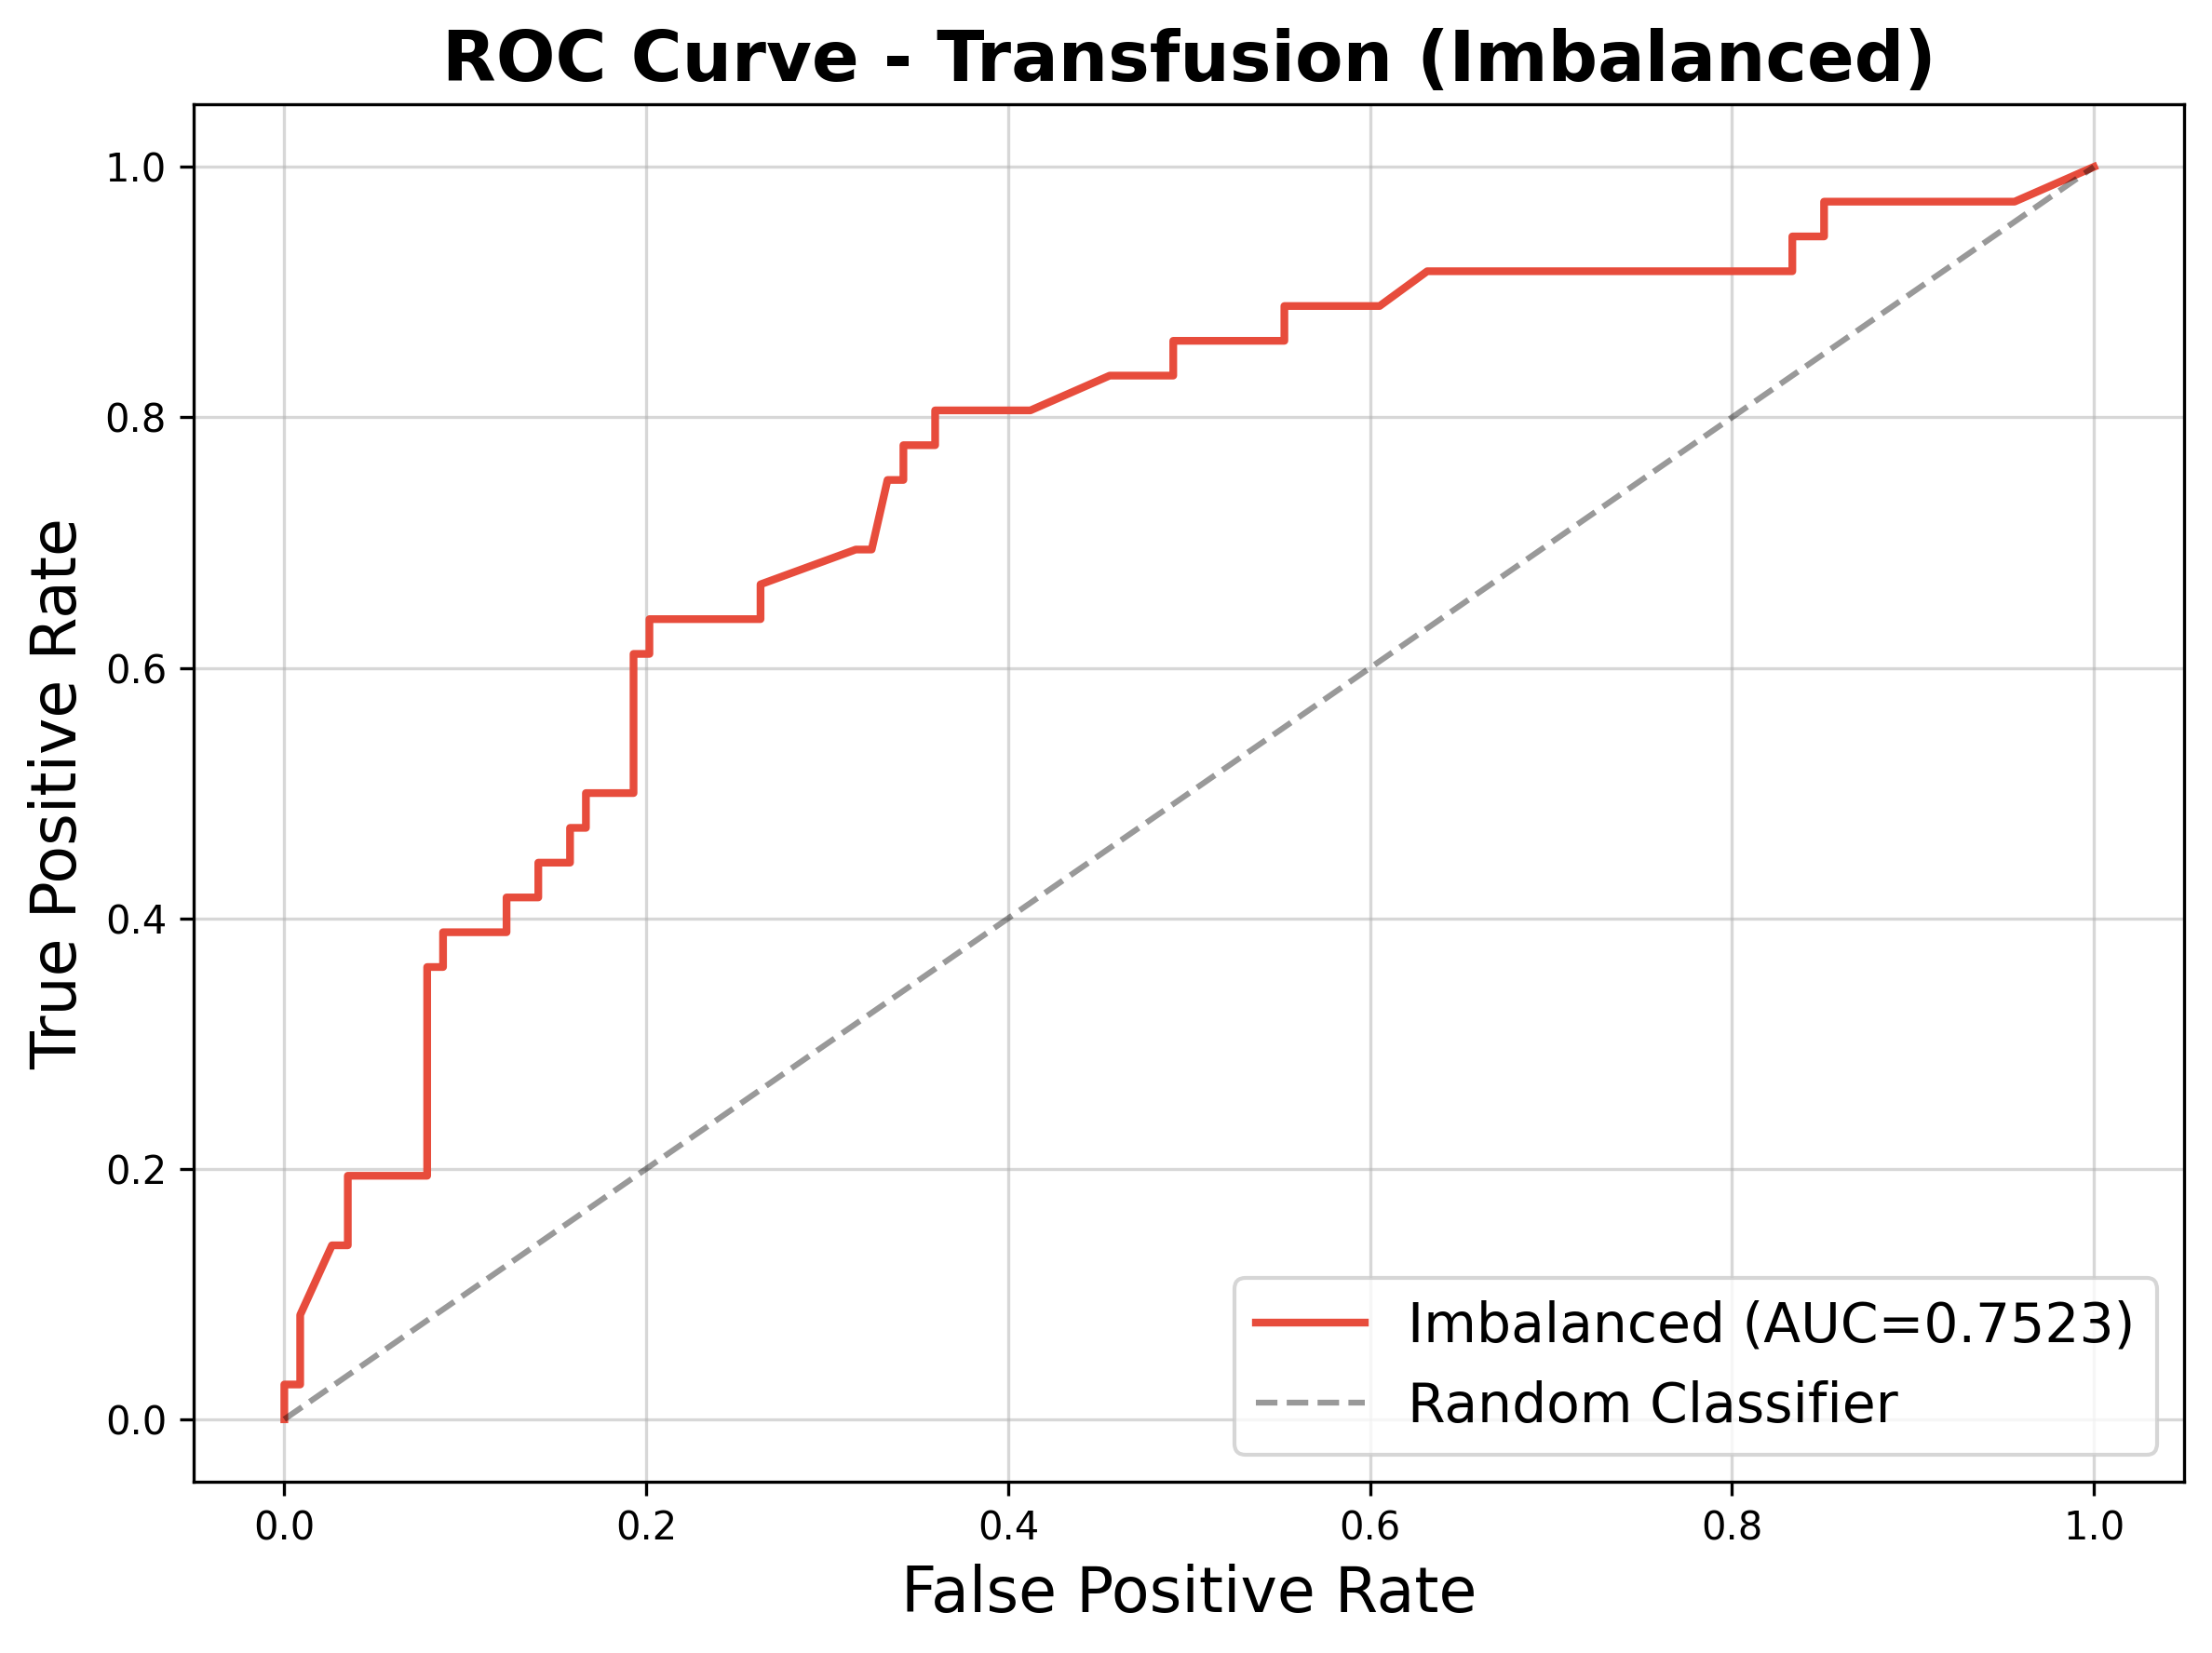
\includegraphics[width=\textwidth]{figure/roc_imbalanced_baseline_transfusion.png}
        \caption{Transfusion}
        \label{fig:4.roc_baseline_transfusion}
    \end{subfigure}

    \vspace{0.5em}

    \begin{subfigure}[b]{0.47\textwidth}
        \centering
        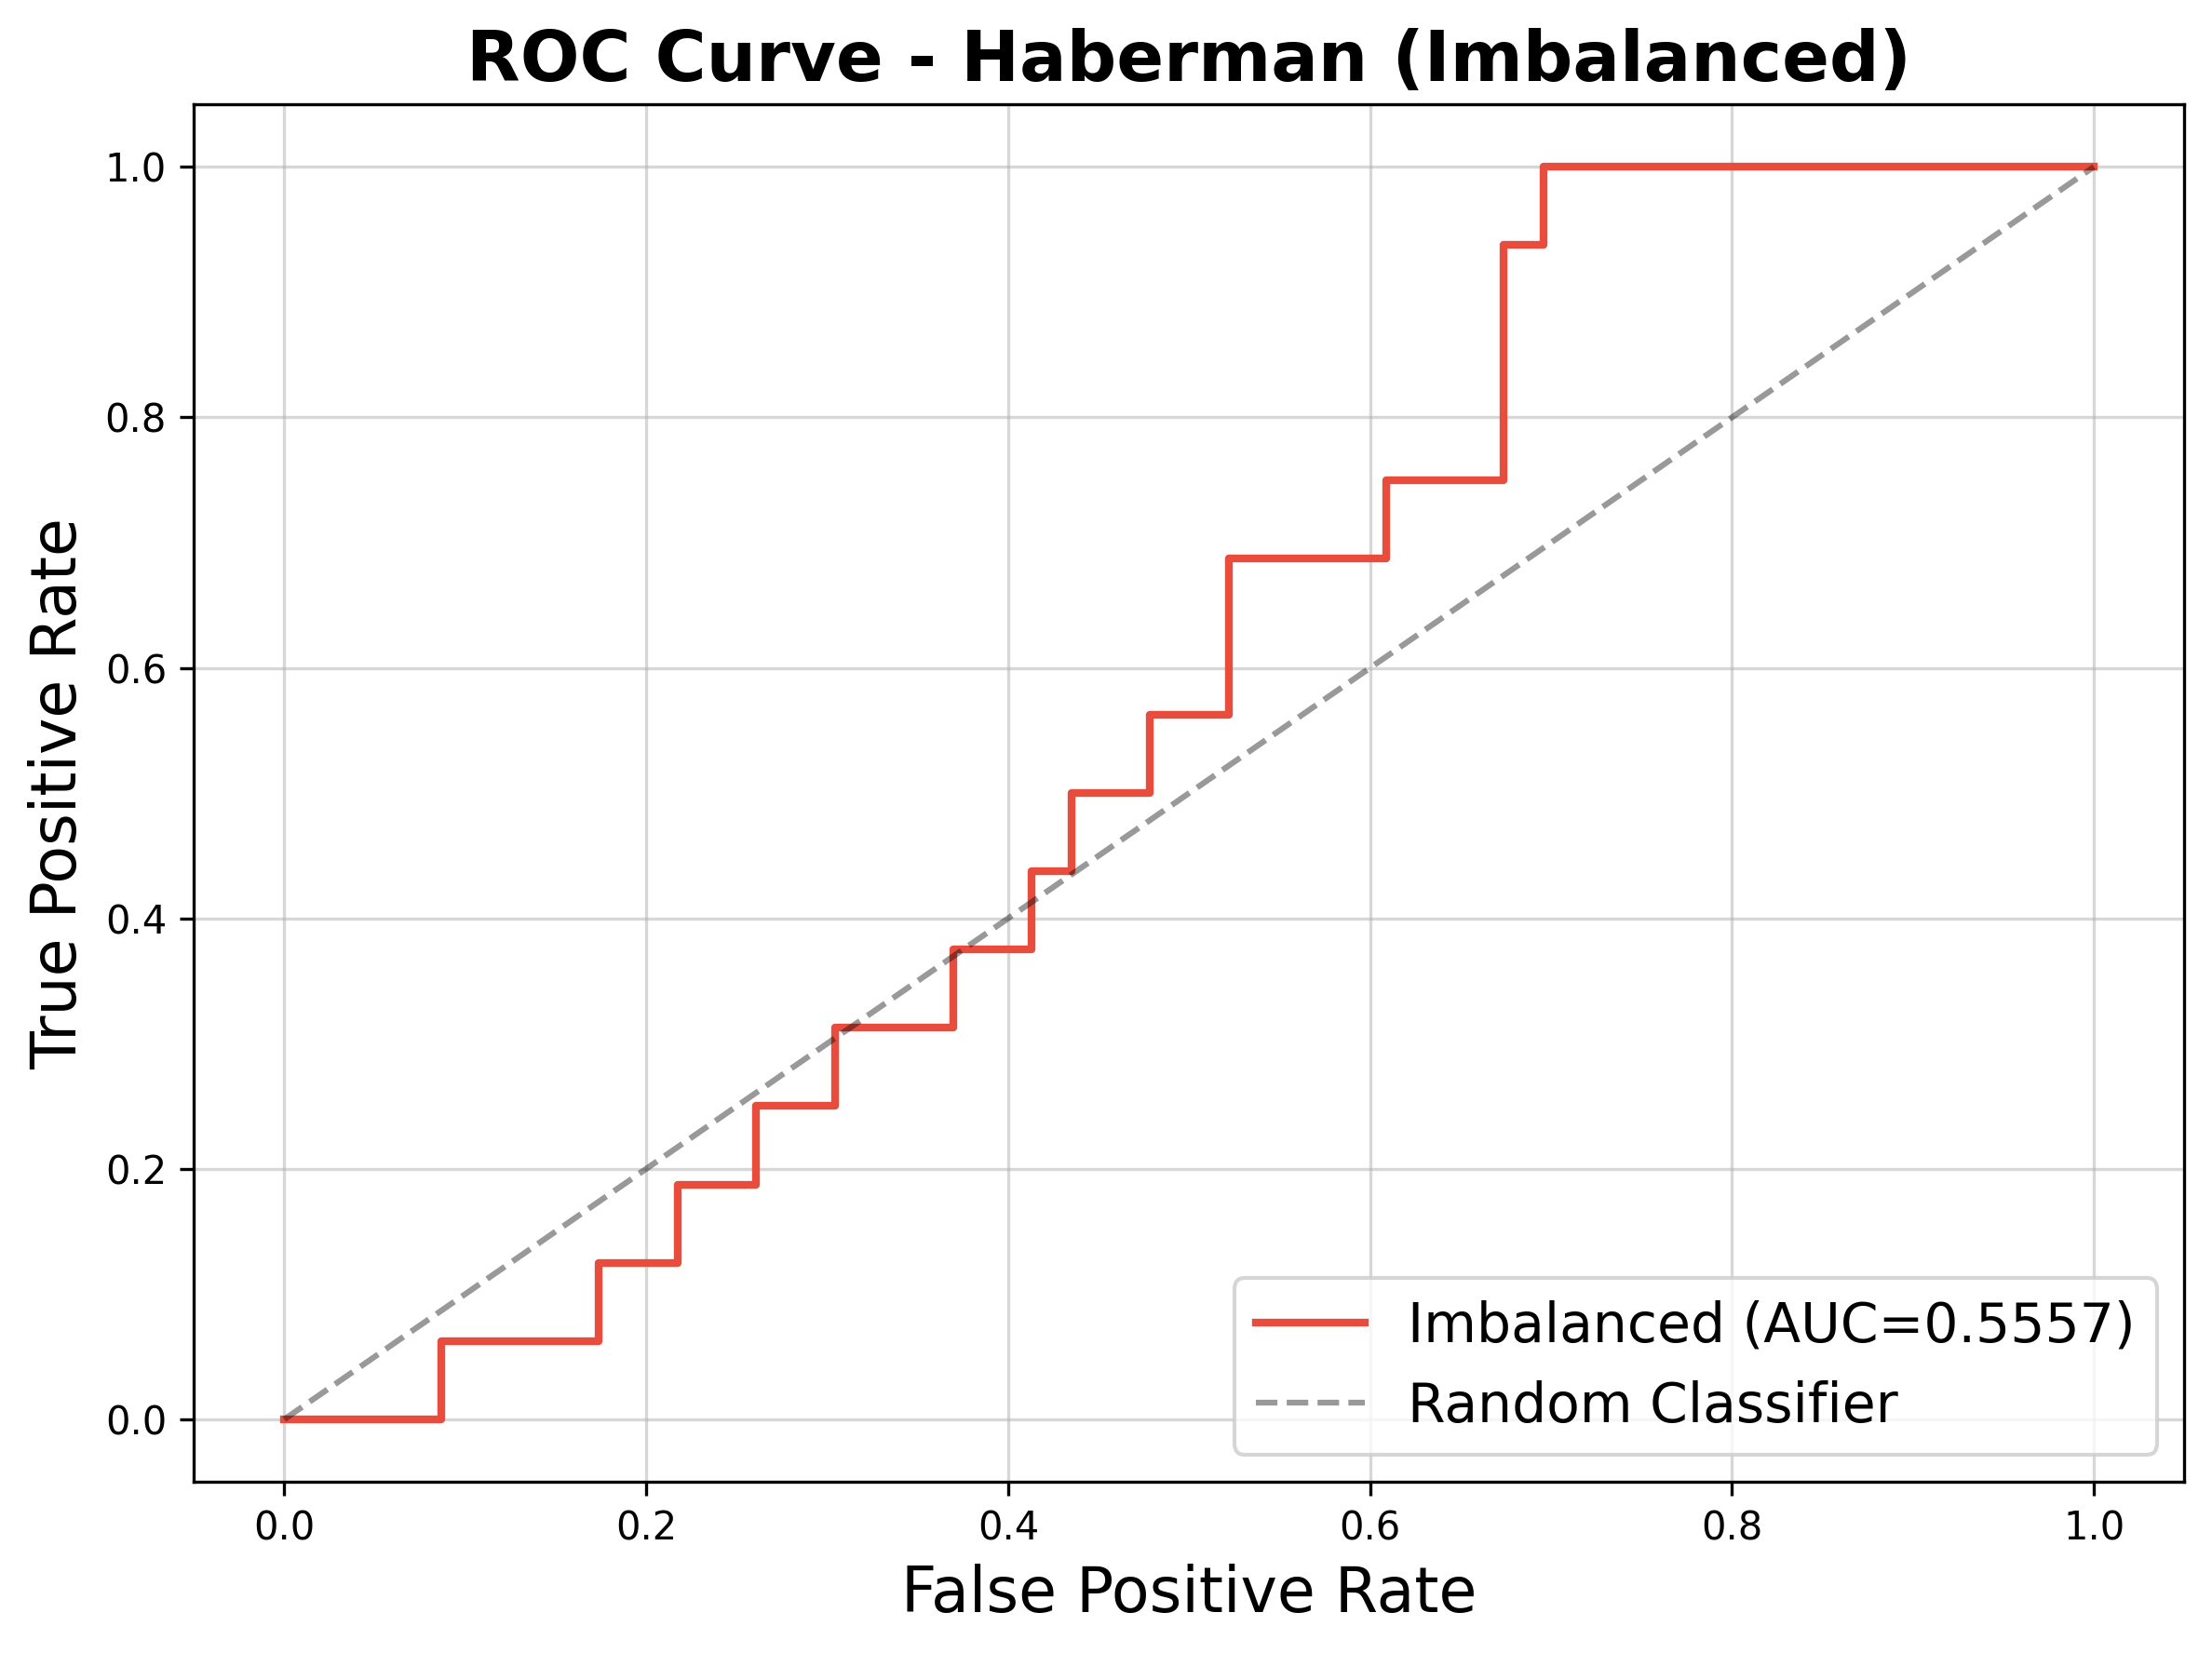
\includegraphics[width=\textwidth]{figure/roc_imbalanced_baseline_haberman.png}
        \caption{Haberman}
        \label{fig:4.roc_baseline_haberman}
    \end{subfigure}
    \hfill
    \begin{subfigure}[b]{0.47\textwidth}
        \centering
        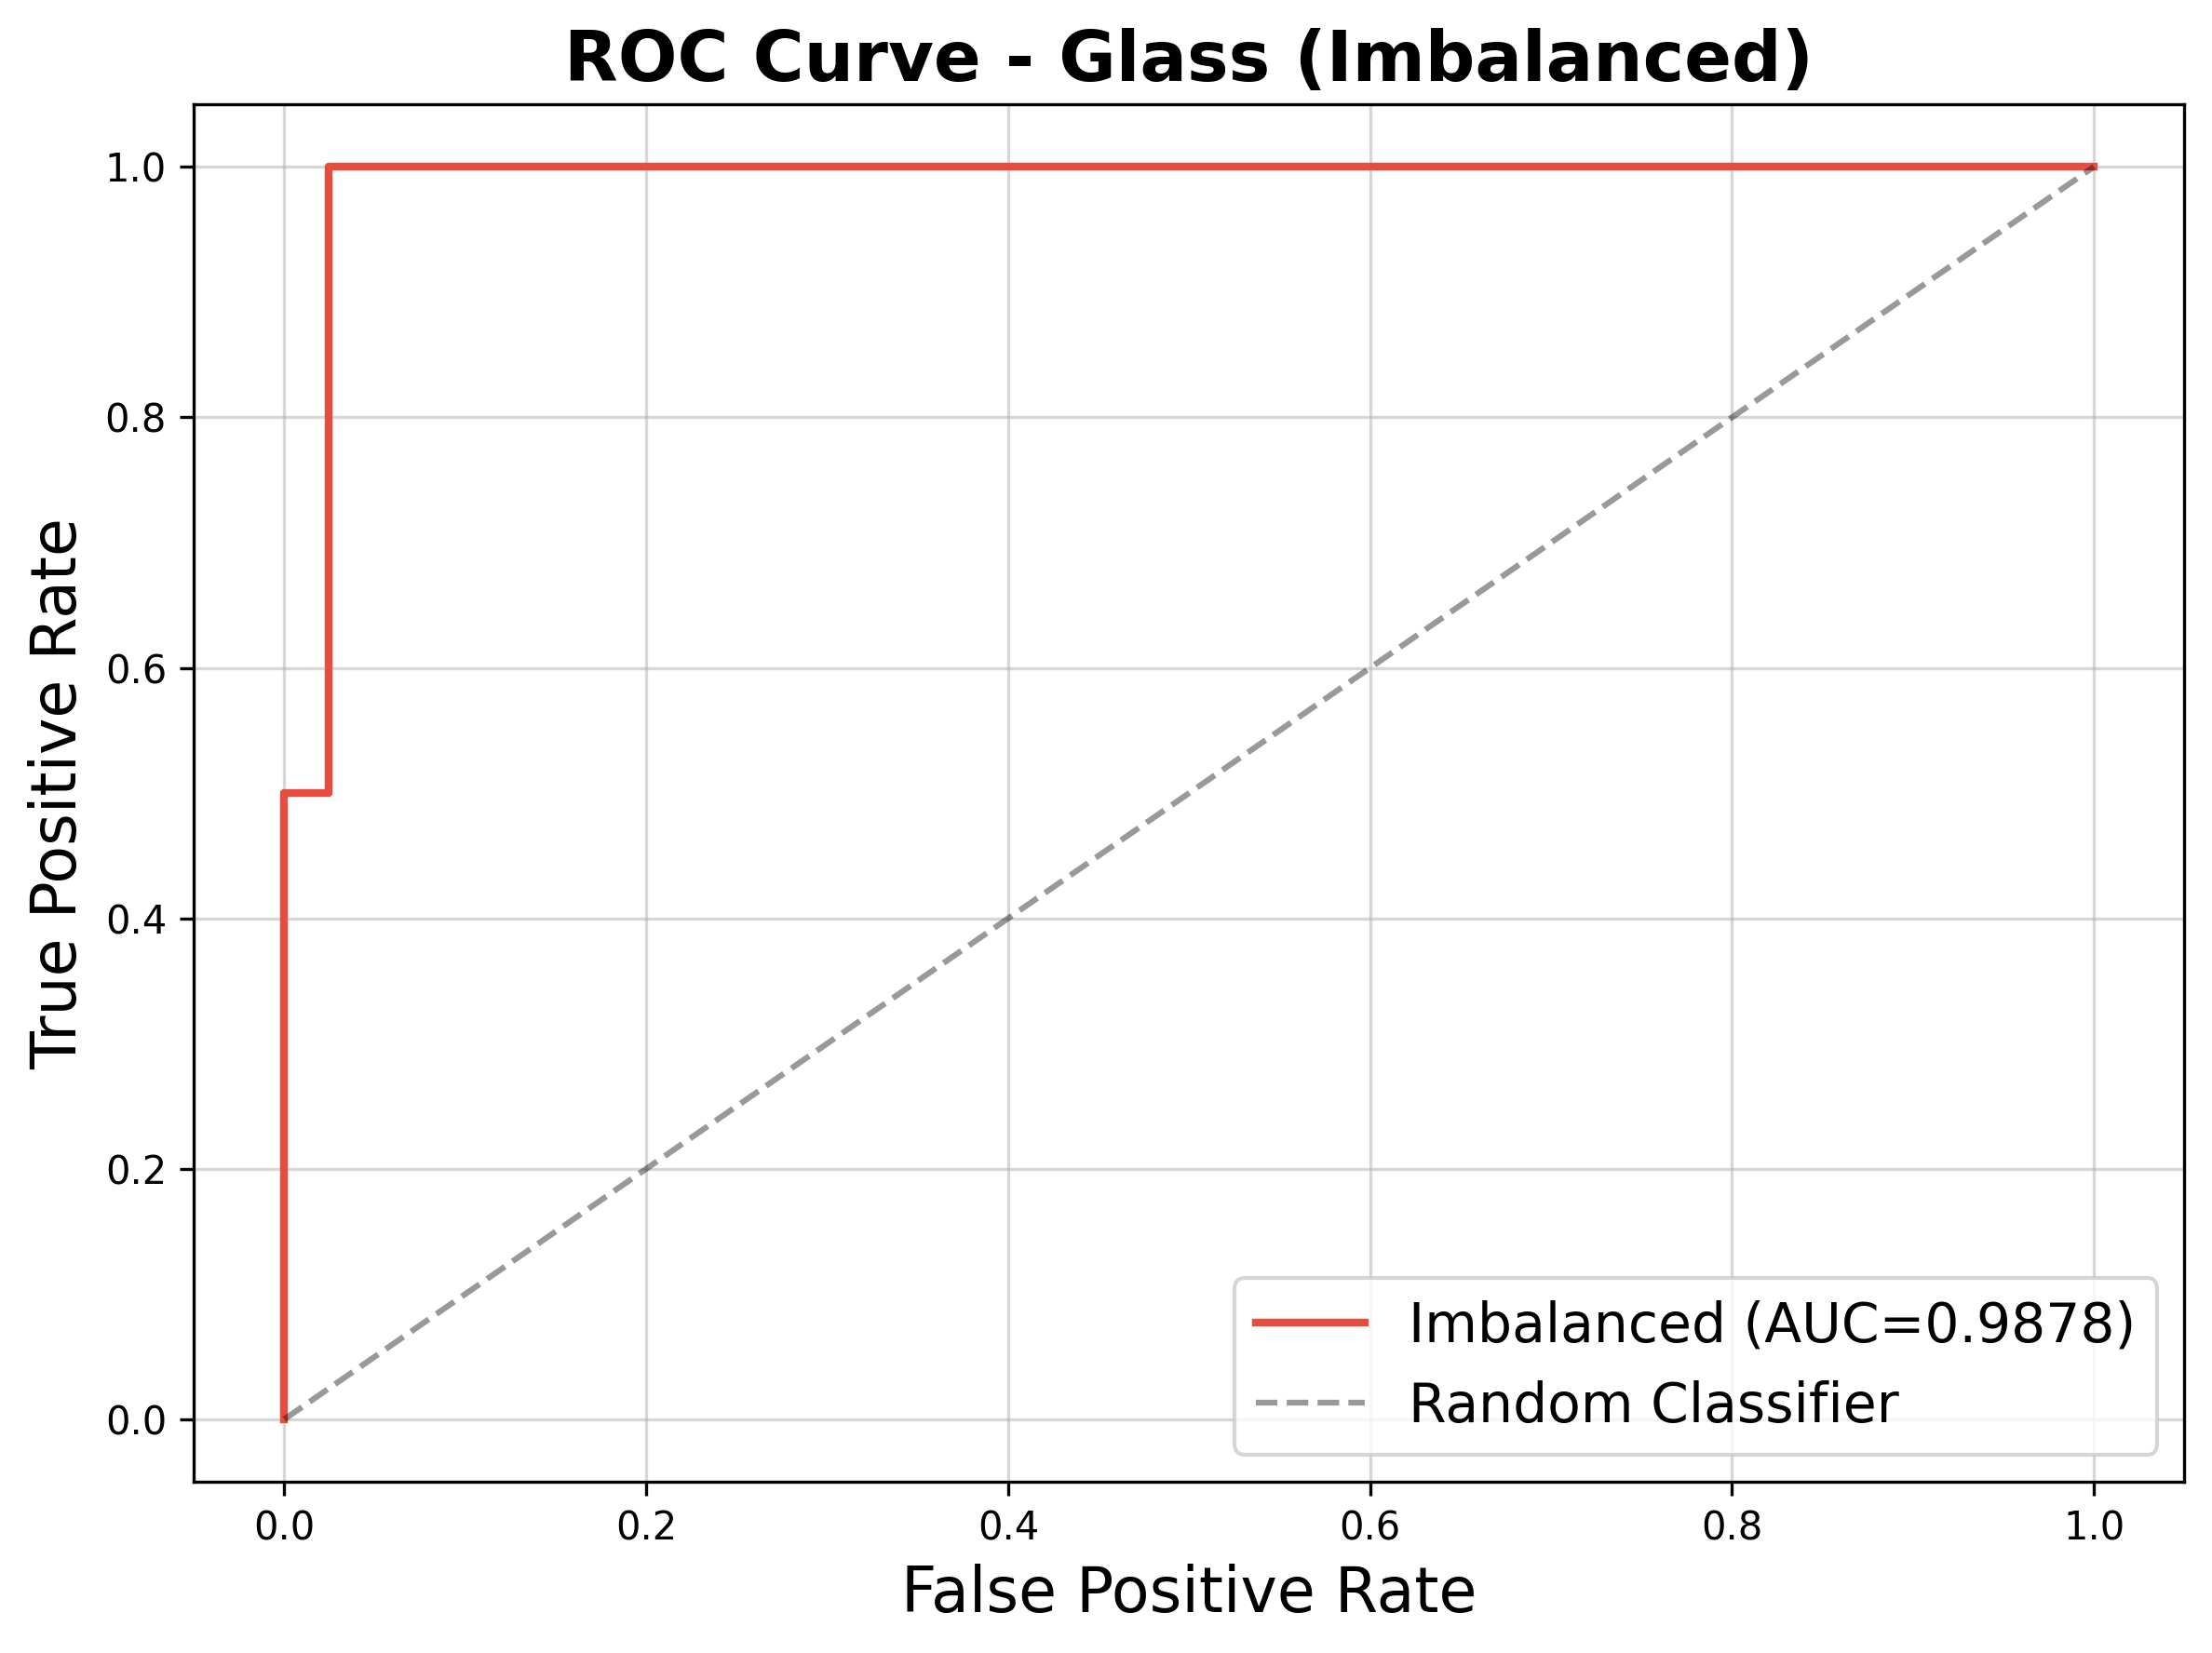
\includegraphics[width=\textwidth]{figure/roc_imbalanced_baseline_glass.png}
        \caption{Glass5}
        \label{fig:4.roc_baseline_glass}
    \end{subfigure}
    \caption{Kurva ROC \textit{Baseline} pada Data Tidak Seimbang}
    \label{fig:4.roc_baseline}
\end{figure}

Berdasarkan Tabel \ref{table:4.baseline} dan Gambar \ref{fig:4.roc_baseline}, model \textit{Random Forest} pada kondisi \textit{baseline} kesulitan mengenali kelas minoritas di seluruh dataset, meskipun dengan tingkat keparahan yang berbeda. Pada dataset Diabetes, nilai ROC-AUC tercatat 0,8194 dan kurva ROC pada Gambar \ref{fig:4.roc_baseline_diabetes} terlihat cukup jauh dari garis diagonal, namun \textit{Recall} hanya mencapai 0,6111 sehingga 39\% pasien diabetes positif gagal terdeteksi. Dataset Transfusion menunjukkan \textit{Recall} sebesar 0,4167 dengan ROC-AUC 0,7523, dimana kurva ROC pada Gambar \ref{fig:4.roc_baseline_transfusion} mendekat ke garis diagonal. Performa terendah terjadi pada dataset Haberman dengan ROC-AUC 0,5557 yang nyaris setara \textit{random classifier} dan \textit{Recall} hanya 0,1250, sebagaimana kurva ROC pada Gambar \ref{fig:4.roc_baseline_haberman} yang hampir berhimpitan dengan garis diagonal. \par

Dataset Glass5 mencatat ROC-AUC 0,9878 dan \textit{Precision} 1,0000, namun \textit{Recall} hanya 0,5000 dengan G-Mean 0,7071. Nilai \textit{Precision} 1,0000 menunjukkan bahwa model tidak menghasilkan satu pun \textit{false positive}, tetapi hanya mendeteksi setengah dari sampel kelas minoritas. Sembilan fitur pada Glass5 memberikan pemisahan yang baik antar kelas, namun jumlah sampel minoritas yang sedikit (9 data) menyebabkan model tidak memiliki cukup data untuk mengenali pola kelas minoritas secara menyeluruh. \par

Pola ini menunjukkan korelasi antara rasio ketidakseimbangan dan performa model. Dataset Diabetes dengan rasio paling rendah (1:1,87) dan delapan fitur menghasilkan kemampuan diskriminatif yang paling memadai, sedangkan Haberman dengan tiga fitur dan rasio 1:2,78 menghasilkan performa terburuk akibat potensi \textit{overlap} antar kelas. Glass5 dengan rasio ekstrem 1:22,78 menghasilkan ROC-AUC sangat tinggi namun \textit{Recall} rendah karena sampel minoritas yang terlalu sedikit. Rendahnya \textit{Recall} dan G-Mean pada seluruh dataset mengindikasikan bahwa model \textit{Random Forest} tanpa penyeimbangan data cenderung bias terhadap kelas mayoritas, sehingga memerlukan penerapan metode seperti HOUM.

\subsection{Hasil Metode HOUM dengan Safe-Level SMOTE (HOUM-SLSMOTE)} \label{IV.HOUM_SLS}
Bagian ini menyajikan hasil klasifikasi setelah data diseimbangkan menggunakan metode HOUM dengan Safe-Level SMOTE sebagai komponen \textit{oversampling}. Seluruh kombinasi parameter SVM (tiga jenis kernel dan enam nilai $C$) diuji pada masing-masing dataset. Hasil metrik evaluasi untuk setiap kombinasi konfigurasi ditampilkan pada tabel berikut, dengan nilai terbaik pada setiap metrik dicetak tebal.

\subsubsection{Dataset Diabetes} \label{IV.SLS_Diabetes}
Hasil klasifikasi HOUM-SLSMOTE pada dataset Diabetes untuk seluruh kombinasi kernel dan nilai $C$ ditunjukkan pada Tabel \ref{table:4.sls_diabetes}.

\begin{table}[H]
\centering
\caption{Hasil HOUM-SLSMOTE pada Dataset Diabetes}
\label{table:4.sls_diabetes}
\footnotesize
\begin{tabular}{|l|c|c|c|c|c|c|}
\hline
\textbf{No} & \textbf{Kernel} & \textbf{C} & \textbf{ROC-AUC} & \textbf{\textit{Recall}} & \textbf{\textit{Precision}} & \textbf{G-Mean} \\
\hline
1 & Linear & 0,5 & 0,7806 & \textbf{0,6481} & 0,5932 & 0,7018 \\
\hline
2 & Linear & 1 & 0,7863 & 0,5926 & 0,6154 & 0,6885 \\
\hline
3 & Linear & 1,5 & 0,7815 & 0,6296 & 0,6667 & 0,7229 \\
\hline
4 & Linear & 2 & 0,7815 & 0,6296 & 0,6667 & 0,7229 \\
\hline
5 & Linear & 2,5 & 0,7787 & 0,6111 & 0,6226 & 0,6992 \\
\hline
6 & Linear & 3 & 0,7789 & \textbf{0,6481} & 0,6364 & 0,7201 \\
\hline
7 & RBF & 0,5 & 0,8191 & \textbf{0,6481} & \textbf{0,6863} & \textbf{0,7379} \\
\hline
8 & RBF & 1 & 0,8146 & 0,6111 & 0,6346 & 0,7036 \\
\hline
9 & RBF & 1,5 & 0,8174 & \textbf{0,6481} & 0,6604 & 0,7290 \\
\hline
10 & RBF & 2 & \textbf{0,8228} & \textbf{0,6481} & \textbf{0,6863} & \textbf{0,7379} \\
\hline
11 & RBF & 2,5 & 0,8135 & 0,6111 & 0,6600 & 0,7122 \\
\hline
12 & RBF & 3 & 0,8120 & 0,6296 & 0,6296 & 0,7097 \\
\hline
13 & Poly & 0,5 & 0,7946 & 0,6111 & 0,6600 & 0,7122 \\
\hline
14 & Poly & 1 & 0,7941 & 0,6111 & 0,6111 & 0,6948 \\
\hline
15 & Poly & 1,5 & 0,7859 & 0,6111 & 0,6346 & 0,7036 \\
\hline
16 & Poly & 2 & 0,7961 & 0,6296 & 0,6296 & 0,7097 \\
\hline
17 & Poly & 2,5 & 0,8013 & 0,6111 & 0,6346 & 0,7036 \\
\hline
18 & Poly & 3 & 0,7870 & 0,6111 & 0,6111 & 0,6948 \\
\hline
\end{tabular}
\end{table}

Kurva ROC untuk masing-masing kernel pada dataset Diabetes ditunjukkan pada Gambar \ref{fig:4.roc_sls_diabetes}.

\begin{figure}[H]
    \centering
    \begin{subfigure}[b]{0.47\textwidth}
        \centering
        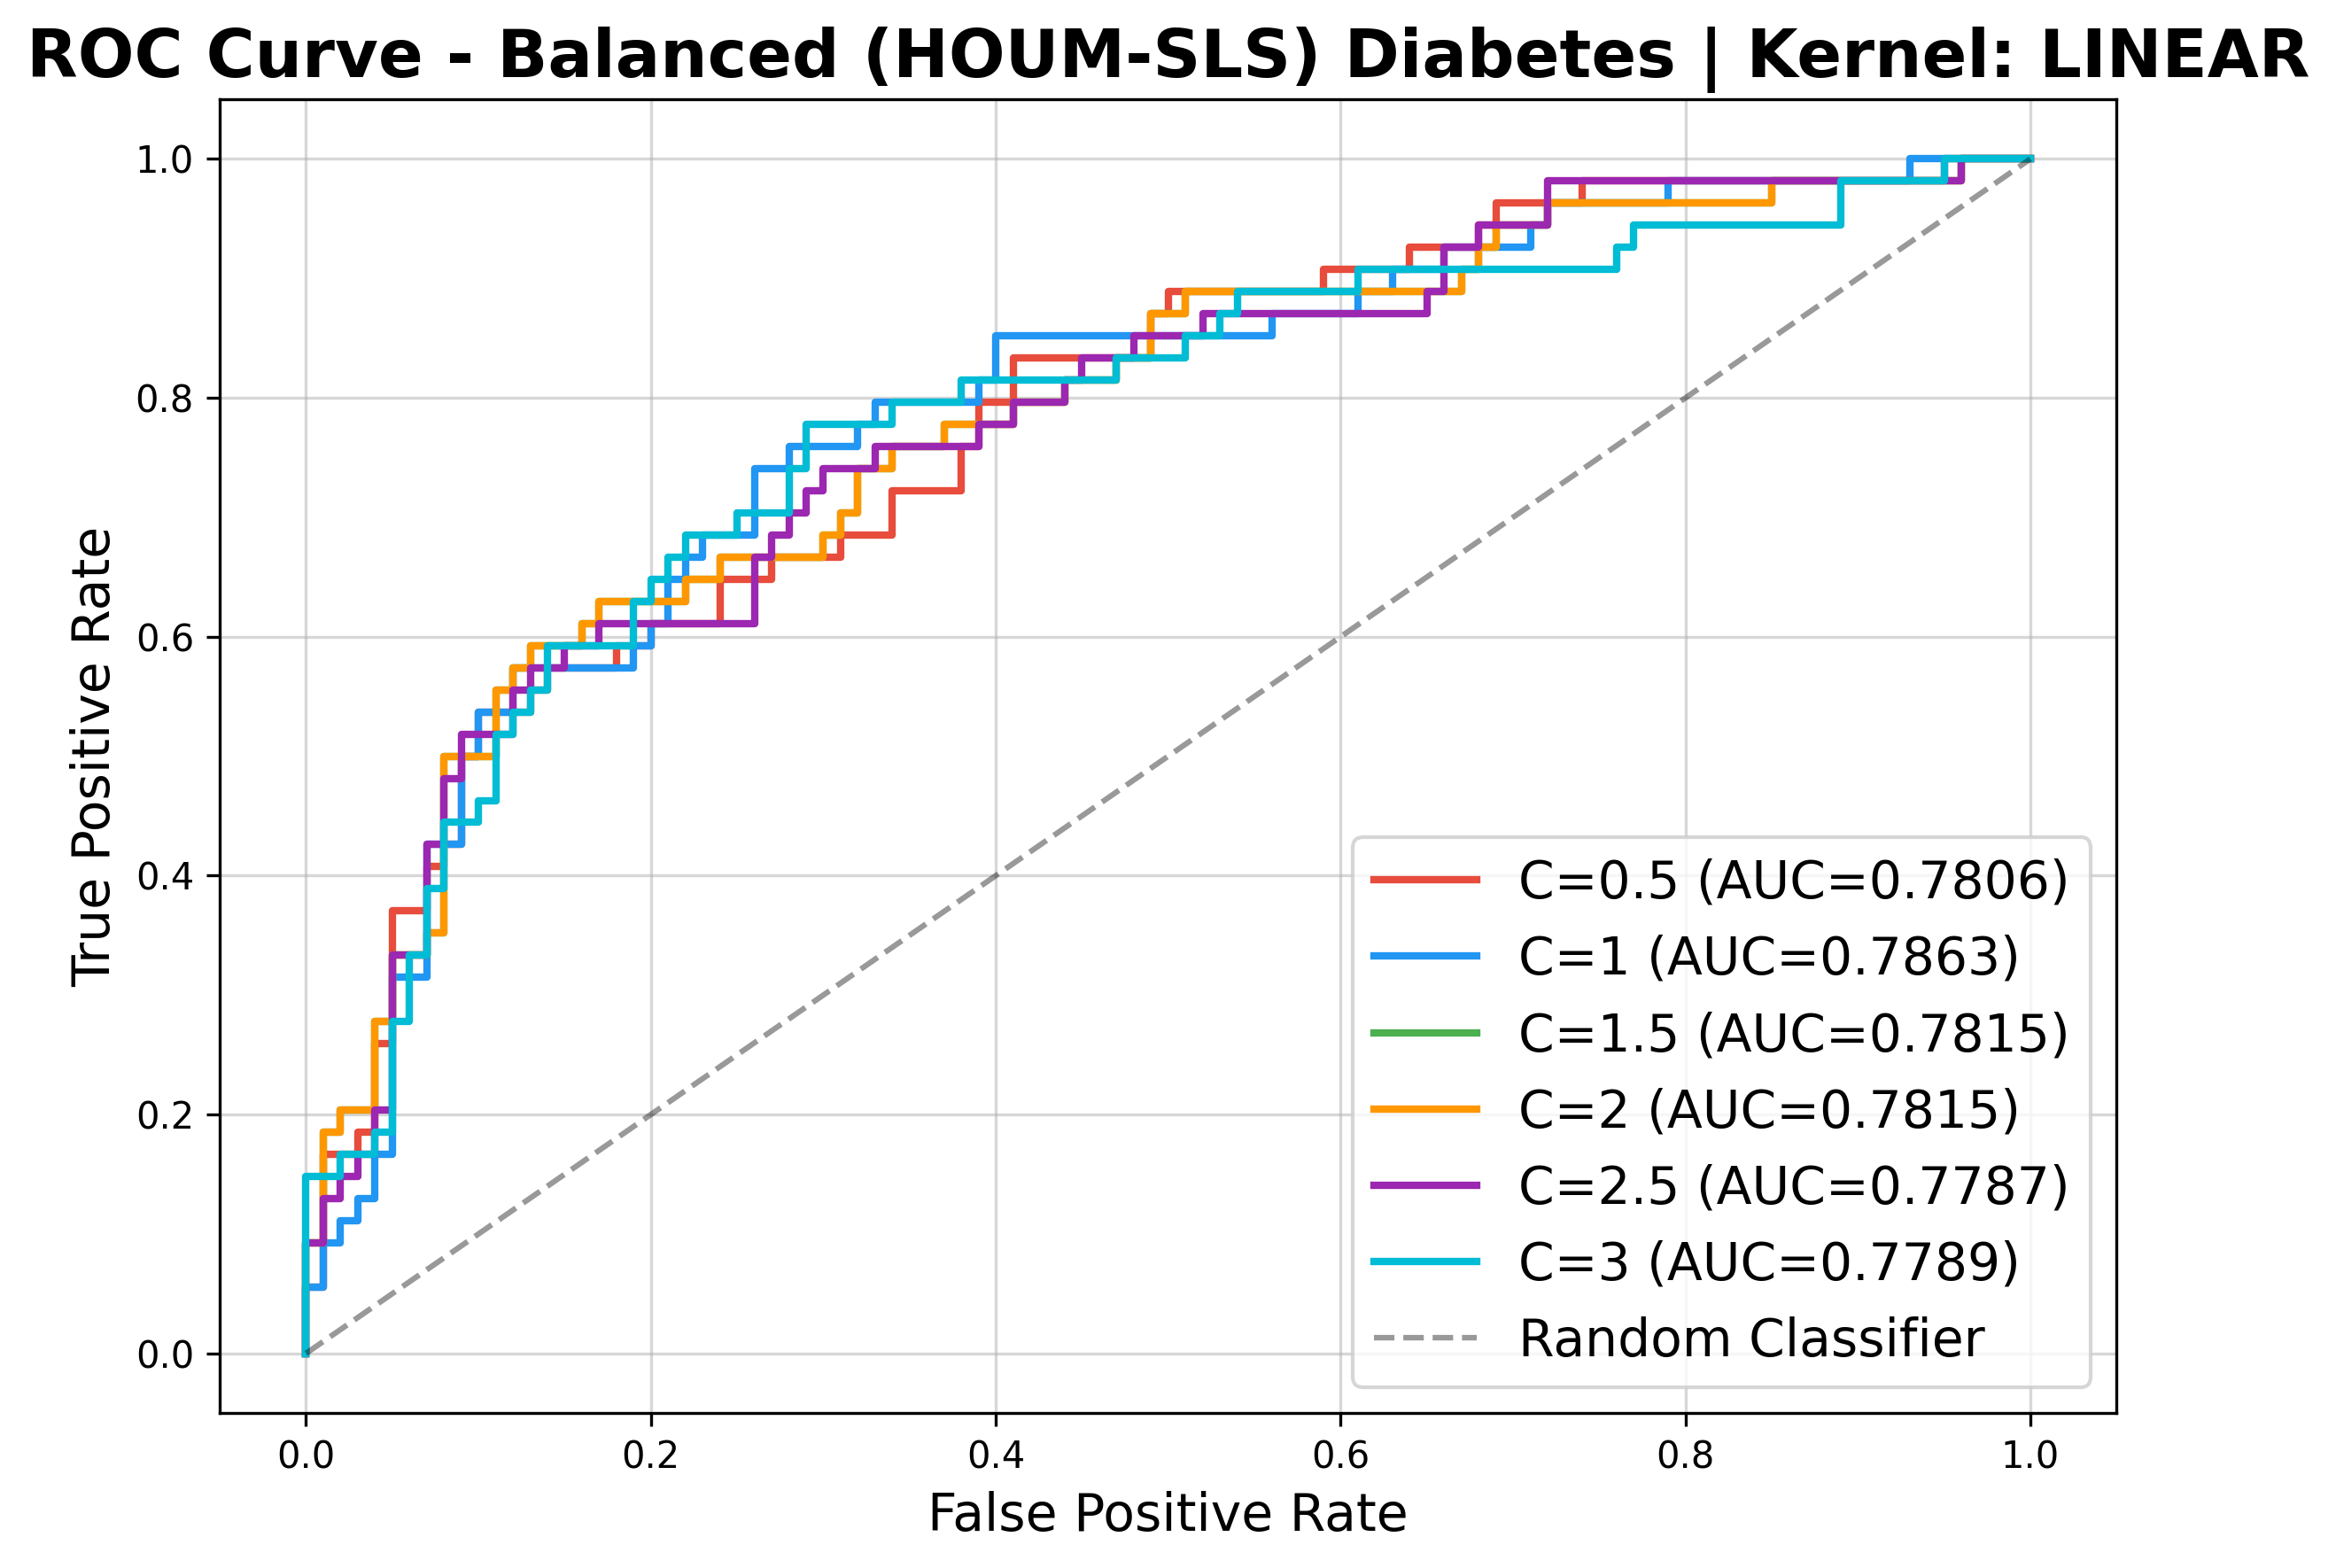
\includegraphics[width=\textwidth]{figure/roc_balanced_diabetes_sls_kernel_linear.png}
        \caption{Kernel Linear}
        \label{fig:4.roc_sls_diabetes_linear}
    \end{subfigure}
    \hfill
    \begin{subfigure}[b]{0.47\textwidth}
        \centering
        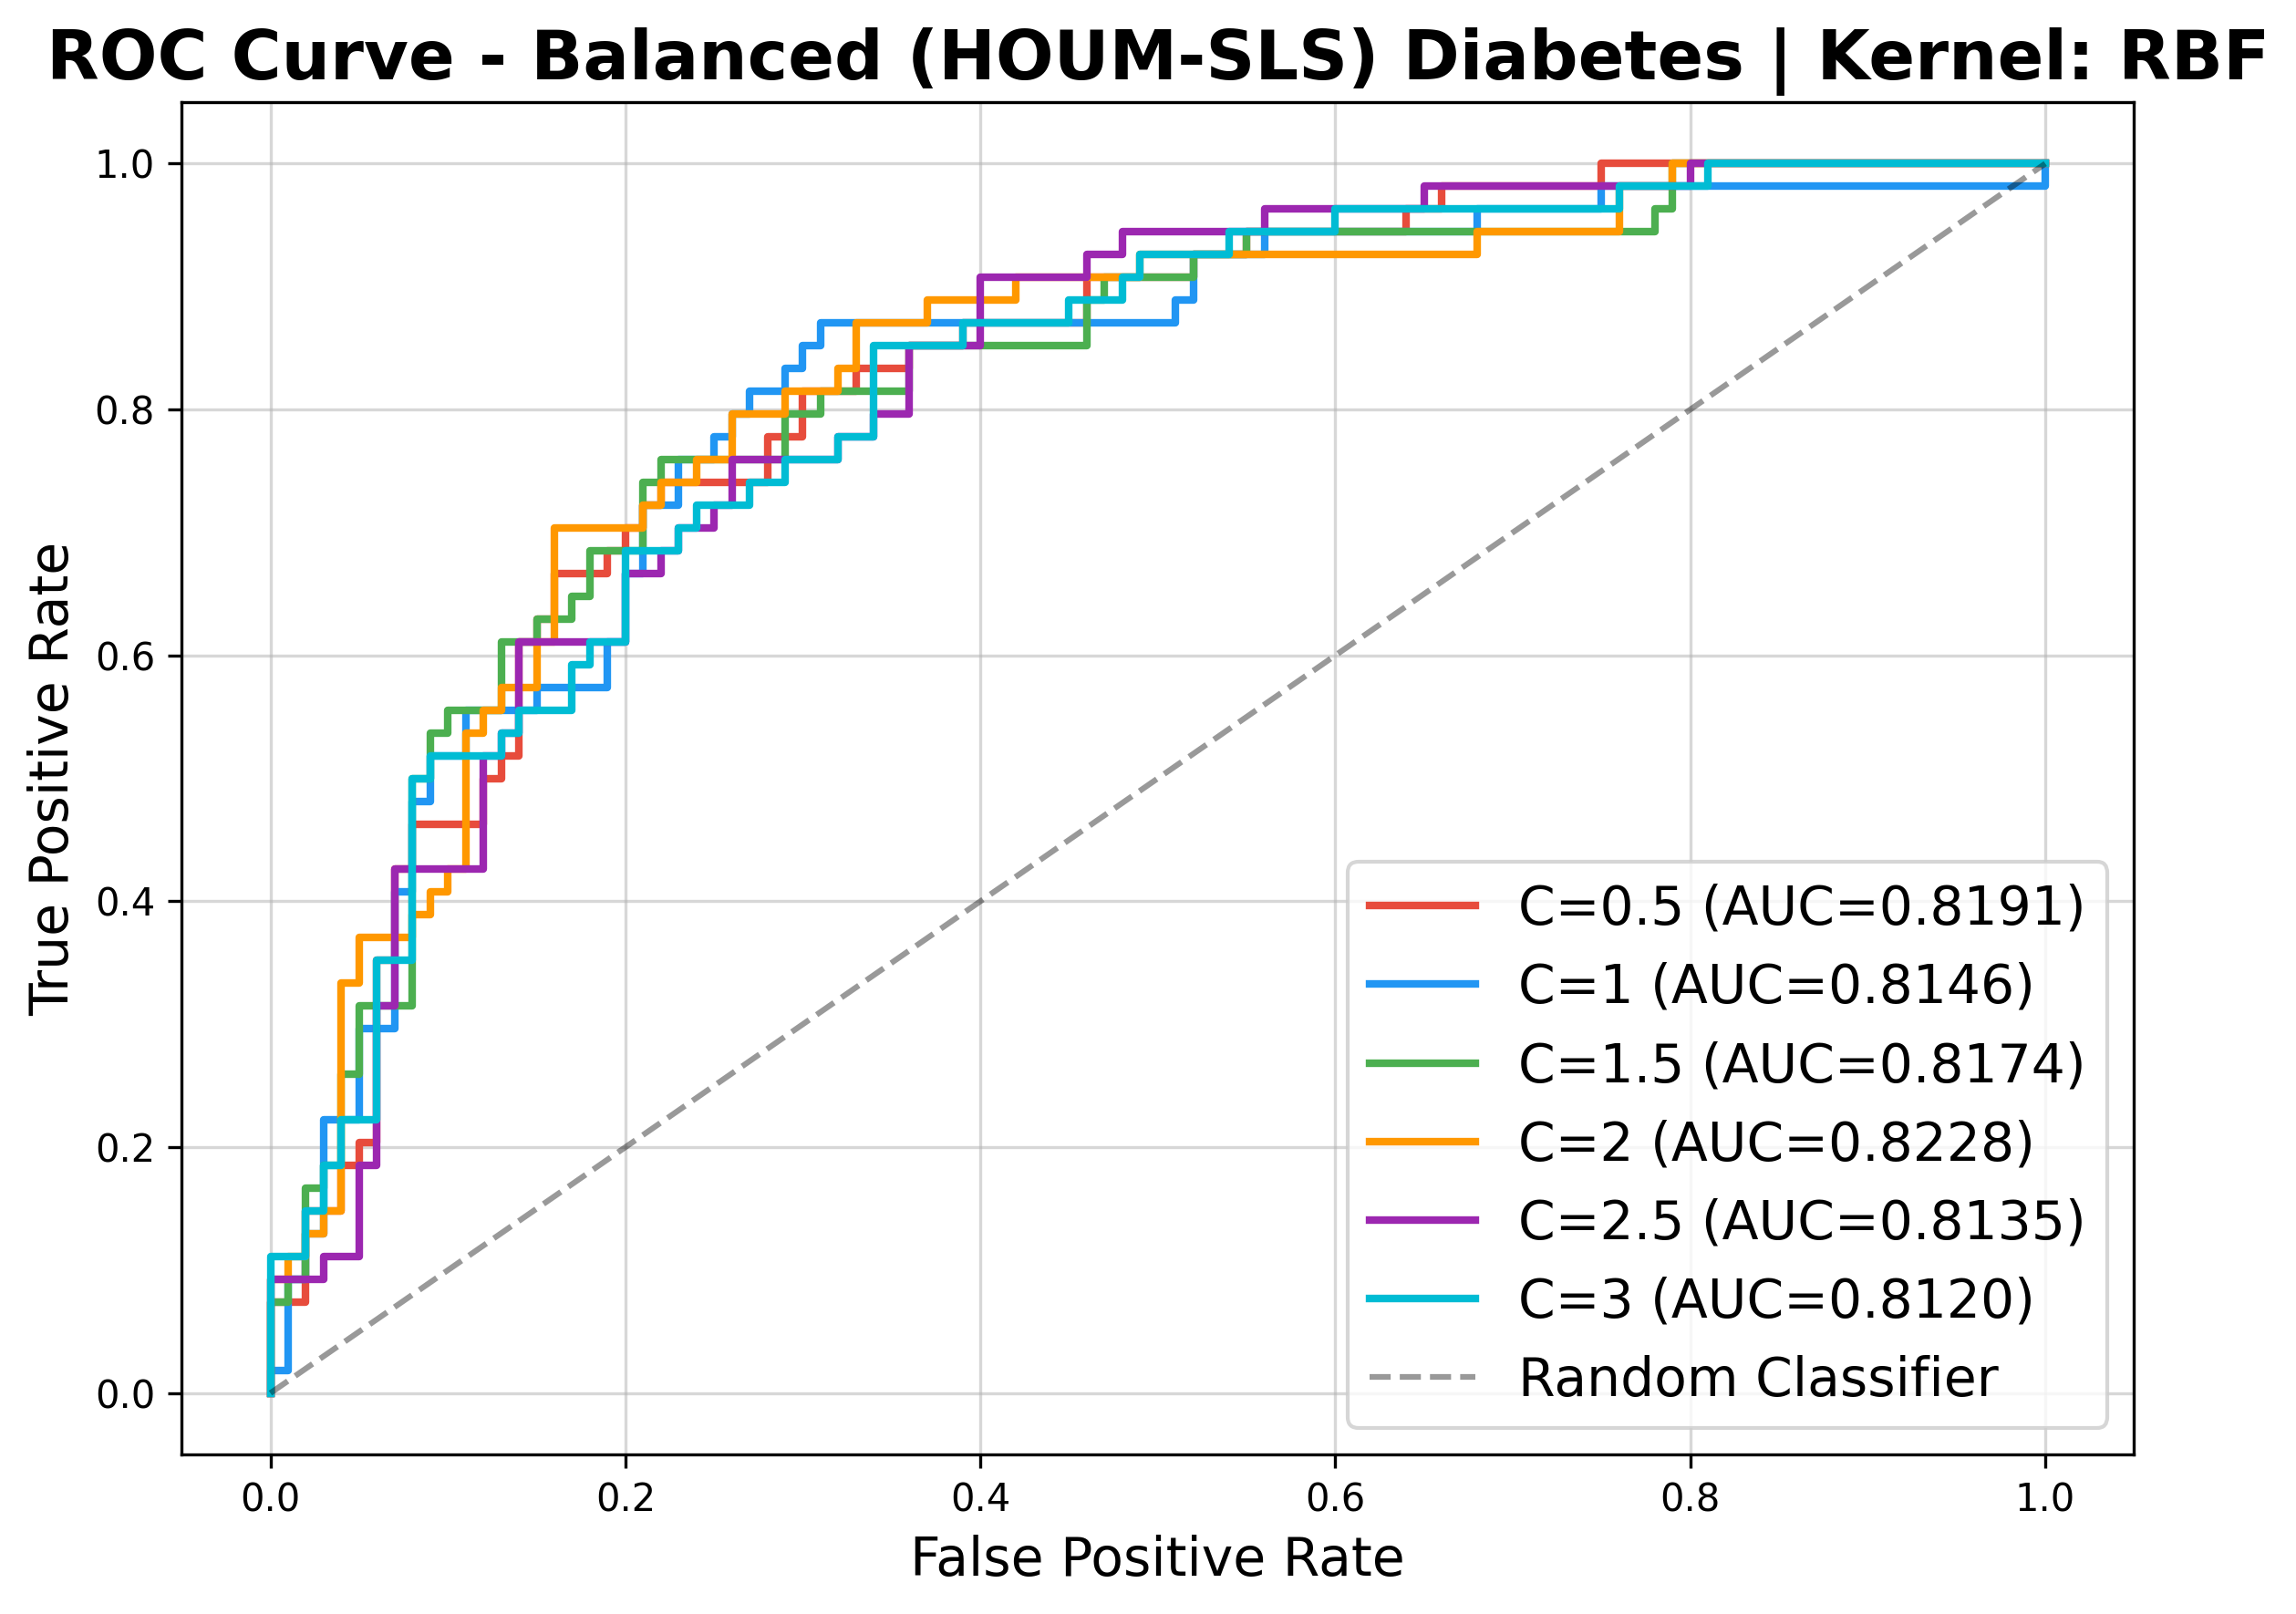
\includegraphics[width=\textwidth]{figure/roc_balanced_diabetes_sls_kernel_rbf.png}
        \caption{Kernel RBF}
        \label{fig:4.roc_sls_diabetes_rbf}
    \end{subfigure}

    \vspace{0.5em}

    \begin{subfigure}[b]{0.47\textwidth}
        \centering
        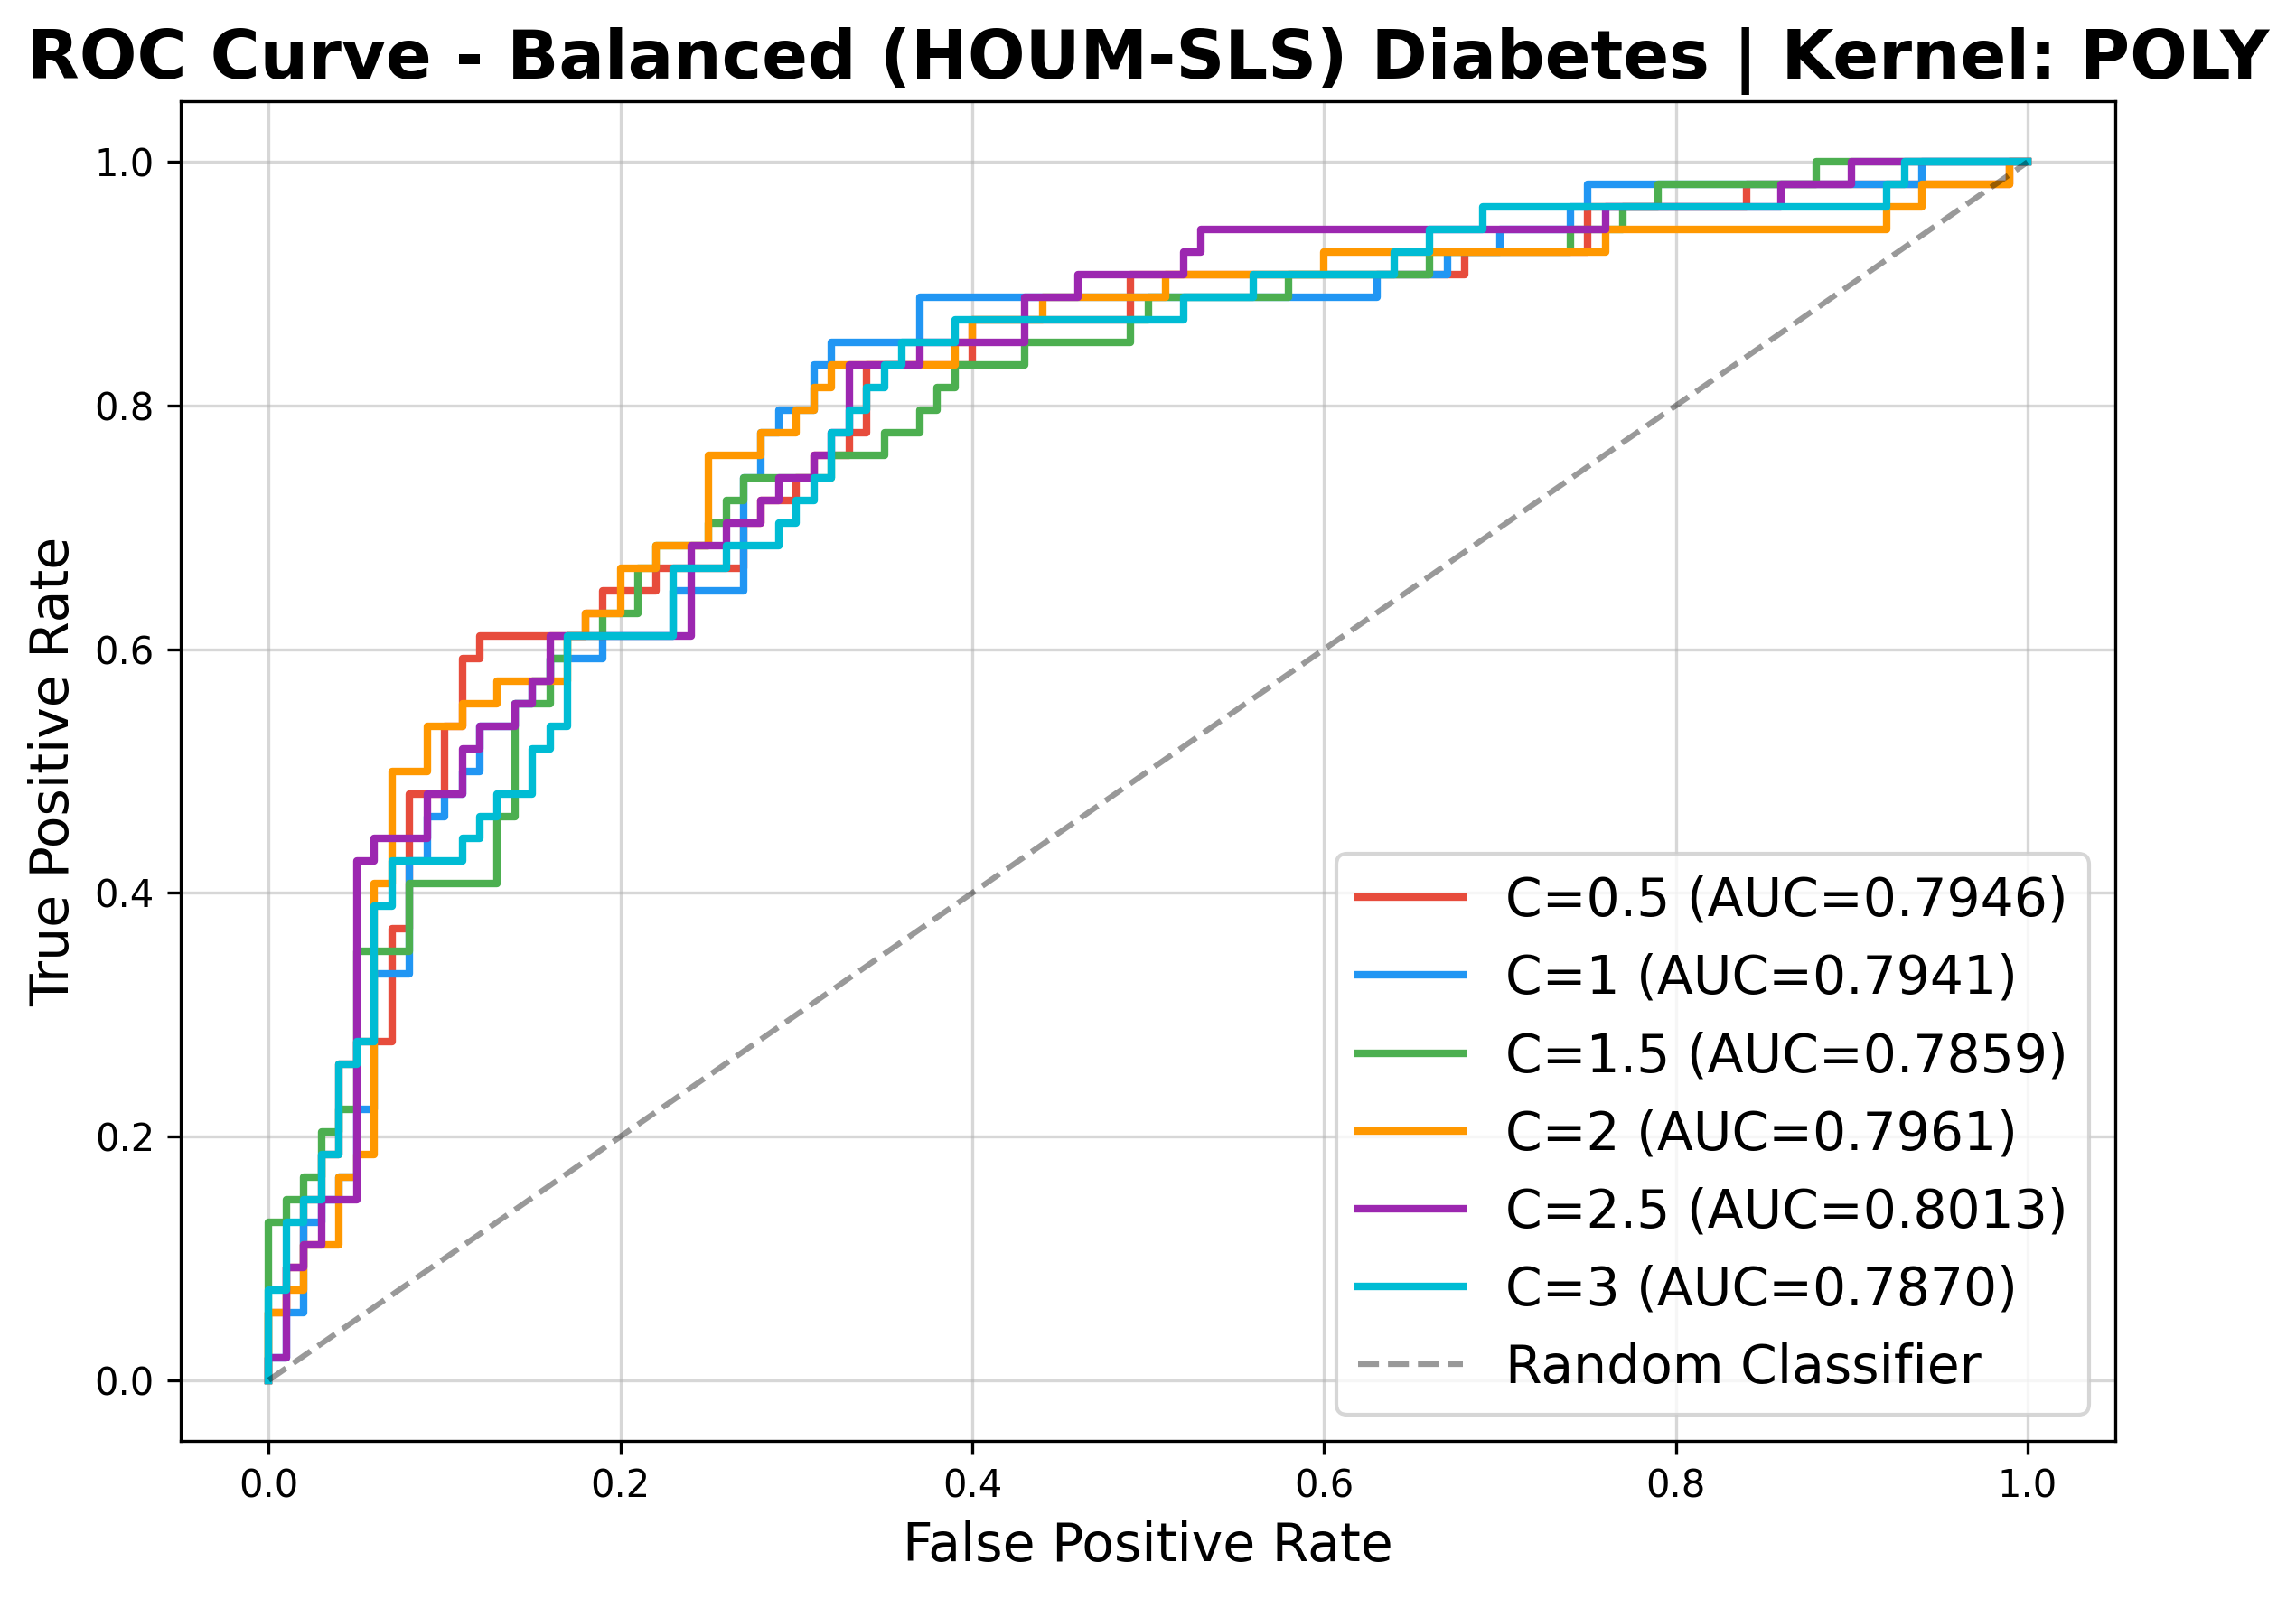
\includegraphics[width=\textwidth]{figure/roc_balanced_diabetes_sls_kernel_poly.png}
        \caption{Kernel Polynomial}
        \label{fig:4.roc_sls_diabetes_poly}
    \end{subfigure}
    \caption{Kurva ROC HOUM-SLSMOTE pada Dataset Diabetes}
    \label{fig:4.roc_sls_diabetes}
\end{figure}

Berdasarkan Tabel \ref{table:4.sls_diabetes}, kernel RBF dengan $C$ = 2 menghasilkan performa terbaik secara keseluruhan dengan ROC-AUC 0,8228, \textit{Precision} 0,6863, dan G-Mean 0,7379. Nilai \textit{Recall} tertinggi sebesar 0,6481 dicapai oleh beberapa konfigurasi kernel Linear dan RBF. Kernel RBF secara konsisten mendominasi pada dataset ini dengan ROC-AUC di atas 0,81 pada seluruh nilai $C$, sedangkan kernel Polynomial stabil namun di bawah RBF, dan kernel Linear mencatat ROC-AUC terendah. Dibandingkan dengan \textit{baseline}, konfigurasi RBF $C$ = 2 mempertahankan ROC-AUC sekaligus menghasilkan G-Mean 0,7379 (dari 0,7079) dan \textit{Precision} 0,6863 (dari 0,6471). \par

\subsubsection{Dataset Haberman} \label{IV.SLS_Haberman}
Hasil klasifikasi HOUM-SLSMOTE pada dataset Haberman untuk seluruh kombinasi kernel dan nilai $C$ ditunjukkan pada Tabel \ref{table:4.sls_haberman}.

\begin{table}[H]
\centering
\caption{Hasil HOUM-SLSMOTE pada Dataset Haberman}
\label{table:4.sls_haberman}
\footnotesize
\begin{tabular}{|l|c|c|c|c|c|c|}
\hline
\textbf{No} & \textbf{Kernel} & \textbf{C} & \textbf{ROC-AUC} & \textbf{\textit{Recall}} & \textbf{\textit{Precision}} & \textbf{G-Mean} \\
\hline
1 & Linear & 0,5 & 0,5788 & \textbf{0,3750} & 0,2500 & \textbf{0,4778} \\
\hline
2 & Linear & 1 & 0,4844 & 0,2500 & 0,2222 & 0,4170 \\
\hline
3 & Linear & 1,5 & 0,4844 & 0,2500 & 0,2222 & 0,4170 \\
\hline
4 & Linear & 2 & 0,5707 & \textbf{0,3750} & 0,2500 & \textbf{0,4778} \\
\hline
5 & Linear & 2,5 & 0,5707 & \textbf{0,3750} & 0,2500 & \textbf{0,4778} \\
\hline
6 & Linear & 3 & 0,5707 & \textbf{0,3750} & 0,2500 & \textbf{0,4778} \\
\hline
7 & RBF & 0,5 & 0,4810 & 0,1875 & 0,2143 & 0,3777 \\
\hline
8 & RBF & 1 & 0,5421 & 0,0625 & 0,0833 & 0,2181 \\
\hline
9 & RBF & 1,5 & \textbf{0,6223} & 0,2500 & \textbf{0,2667} & 0,4361 \\
\hline
10 & RBF & 2 & 0,5707 & 0,1250 & 0,1429 & 0,3040 \\
\hline
11 & RBF & 2,5 & 0,5557 & 0,2500 & 0,2353 & 0,4235 \\
\hline
12 & RBF & 3 & 0,5082 & 0,1250 & 0,1250 & 0,2949 \\
\hline
13 & Poly & 0,5 & 0,3961 & 0,2500 & 0,1538 & 0,3612 \\
\hline
14 & Poly & 1 & 0,3791 & 0,2500 & 0,1481 & 0,3536 \\
\hline
15 & Poly & 1,5 & 0,3791 & 0,2500 & 0,1481 & 0,3536 \\
\hline
16 & Poly & 2 & 0,3791 & 0,2500 & 0,1481 & 0,3536 \\
\hline
17 & Poly & 2,5 & 0,3791 & 0,2500 & 0,1481 & 0,3536 \\
\hline
18 & Poly & 3 & 0,3791 & 0,2500 & 0,1481 & 0,3536 \\
\hline
\end{tabular}
\end{table}

Kurva ROC untuk masing-masing kernel pada dataset Haberman ditunjukkan pada Gambar \ref{fig:4.roc_sls_haberman}.

\begin{figure}[H]
    \centering
    \begin{subfigure}[b]{0.47\textwidth}
        \centering
        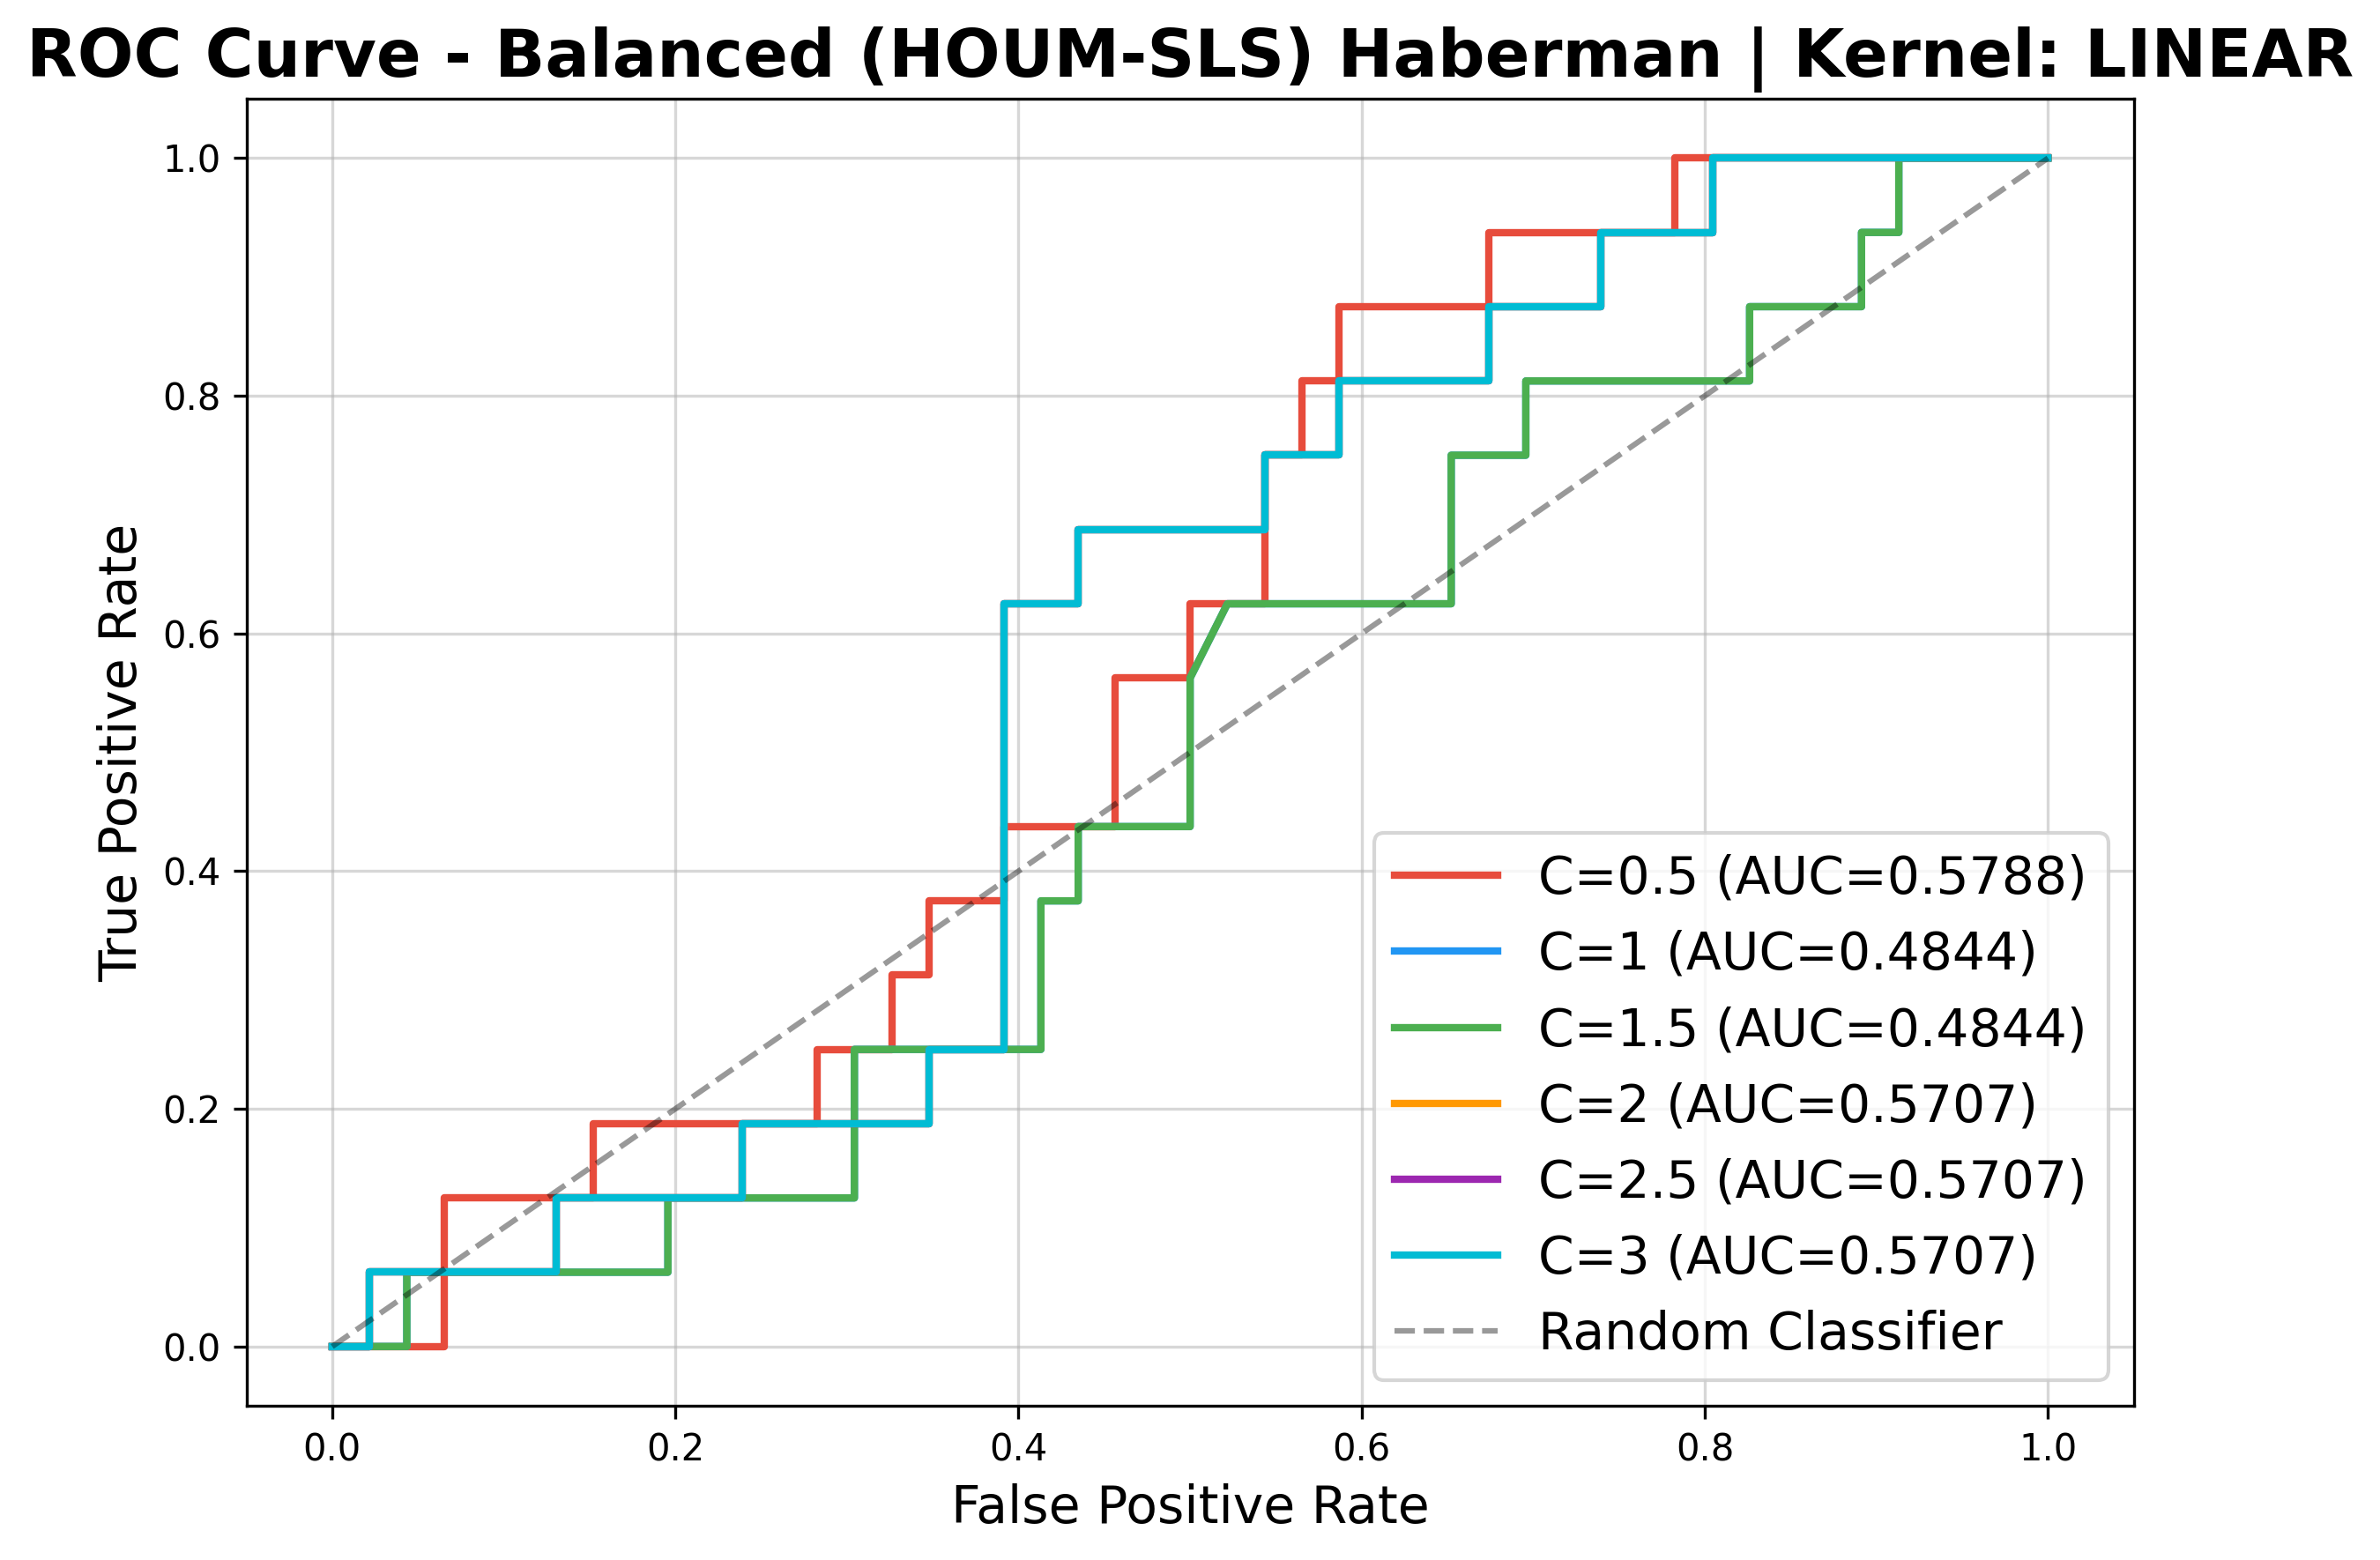
\includegraphics[width=\textwidth]{figure/roc_balanced_haberman_sls_kernel_linear.png}
        \caption{Kernel Linear}
        \label{fig:4.roc_sls_haberman_linear}
    \end{subfigure}
    \hfill
    \begin{subfigure}[b]{0.47\textwidth}
        \centering
        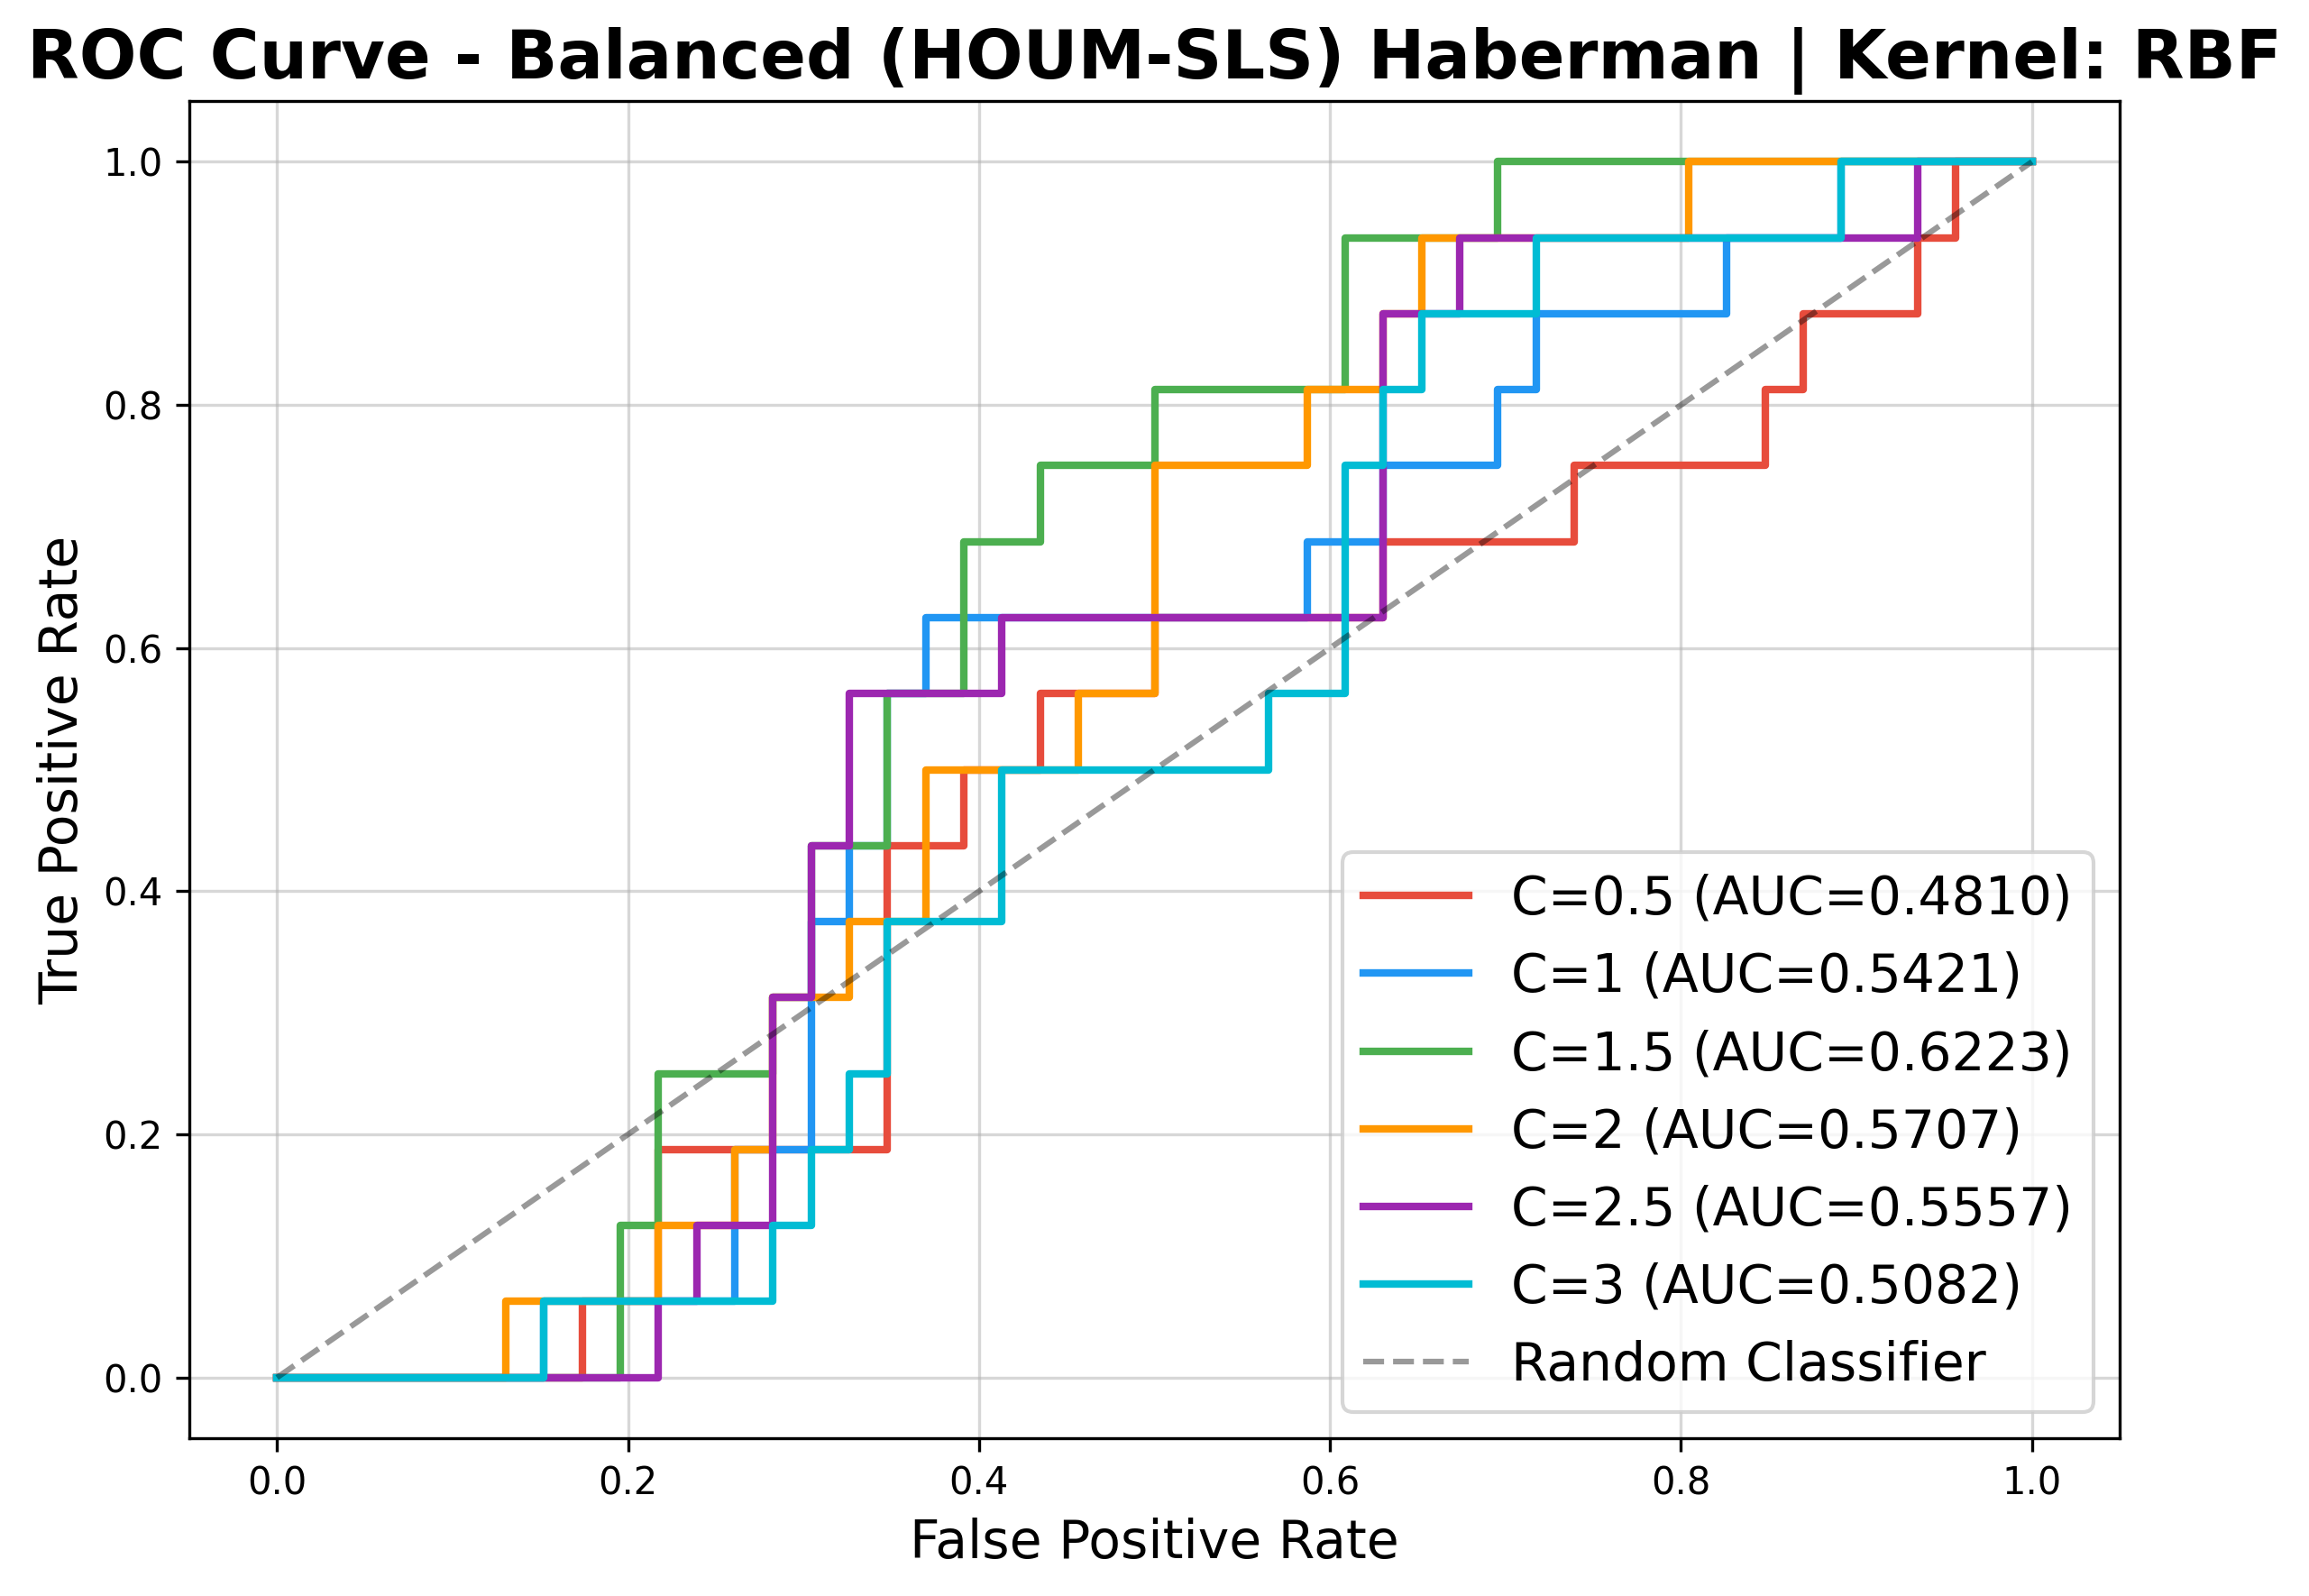
\includegraphics[width=\textwidth]{figure/roc_balanced_haberman_sls_kernel_rbf.png}
        \caption{Kernel RBF}
        \label{fig:4.roc_sls_haberman_rbf}
    \end{subfigure}

    \vspace{0.5em}

    \begin{subfigure}[b]{0.47\textwidth}
        \centering
        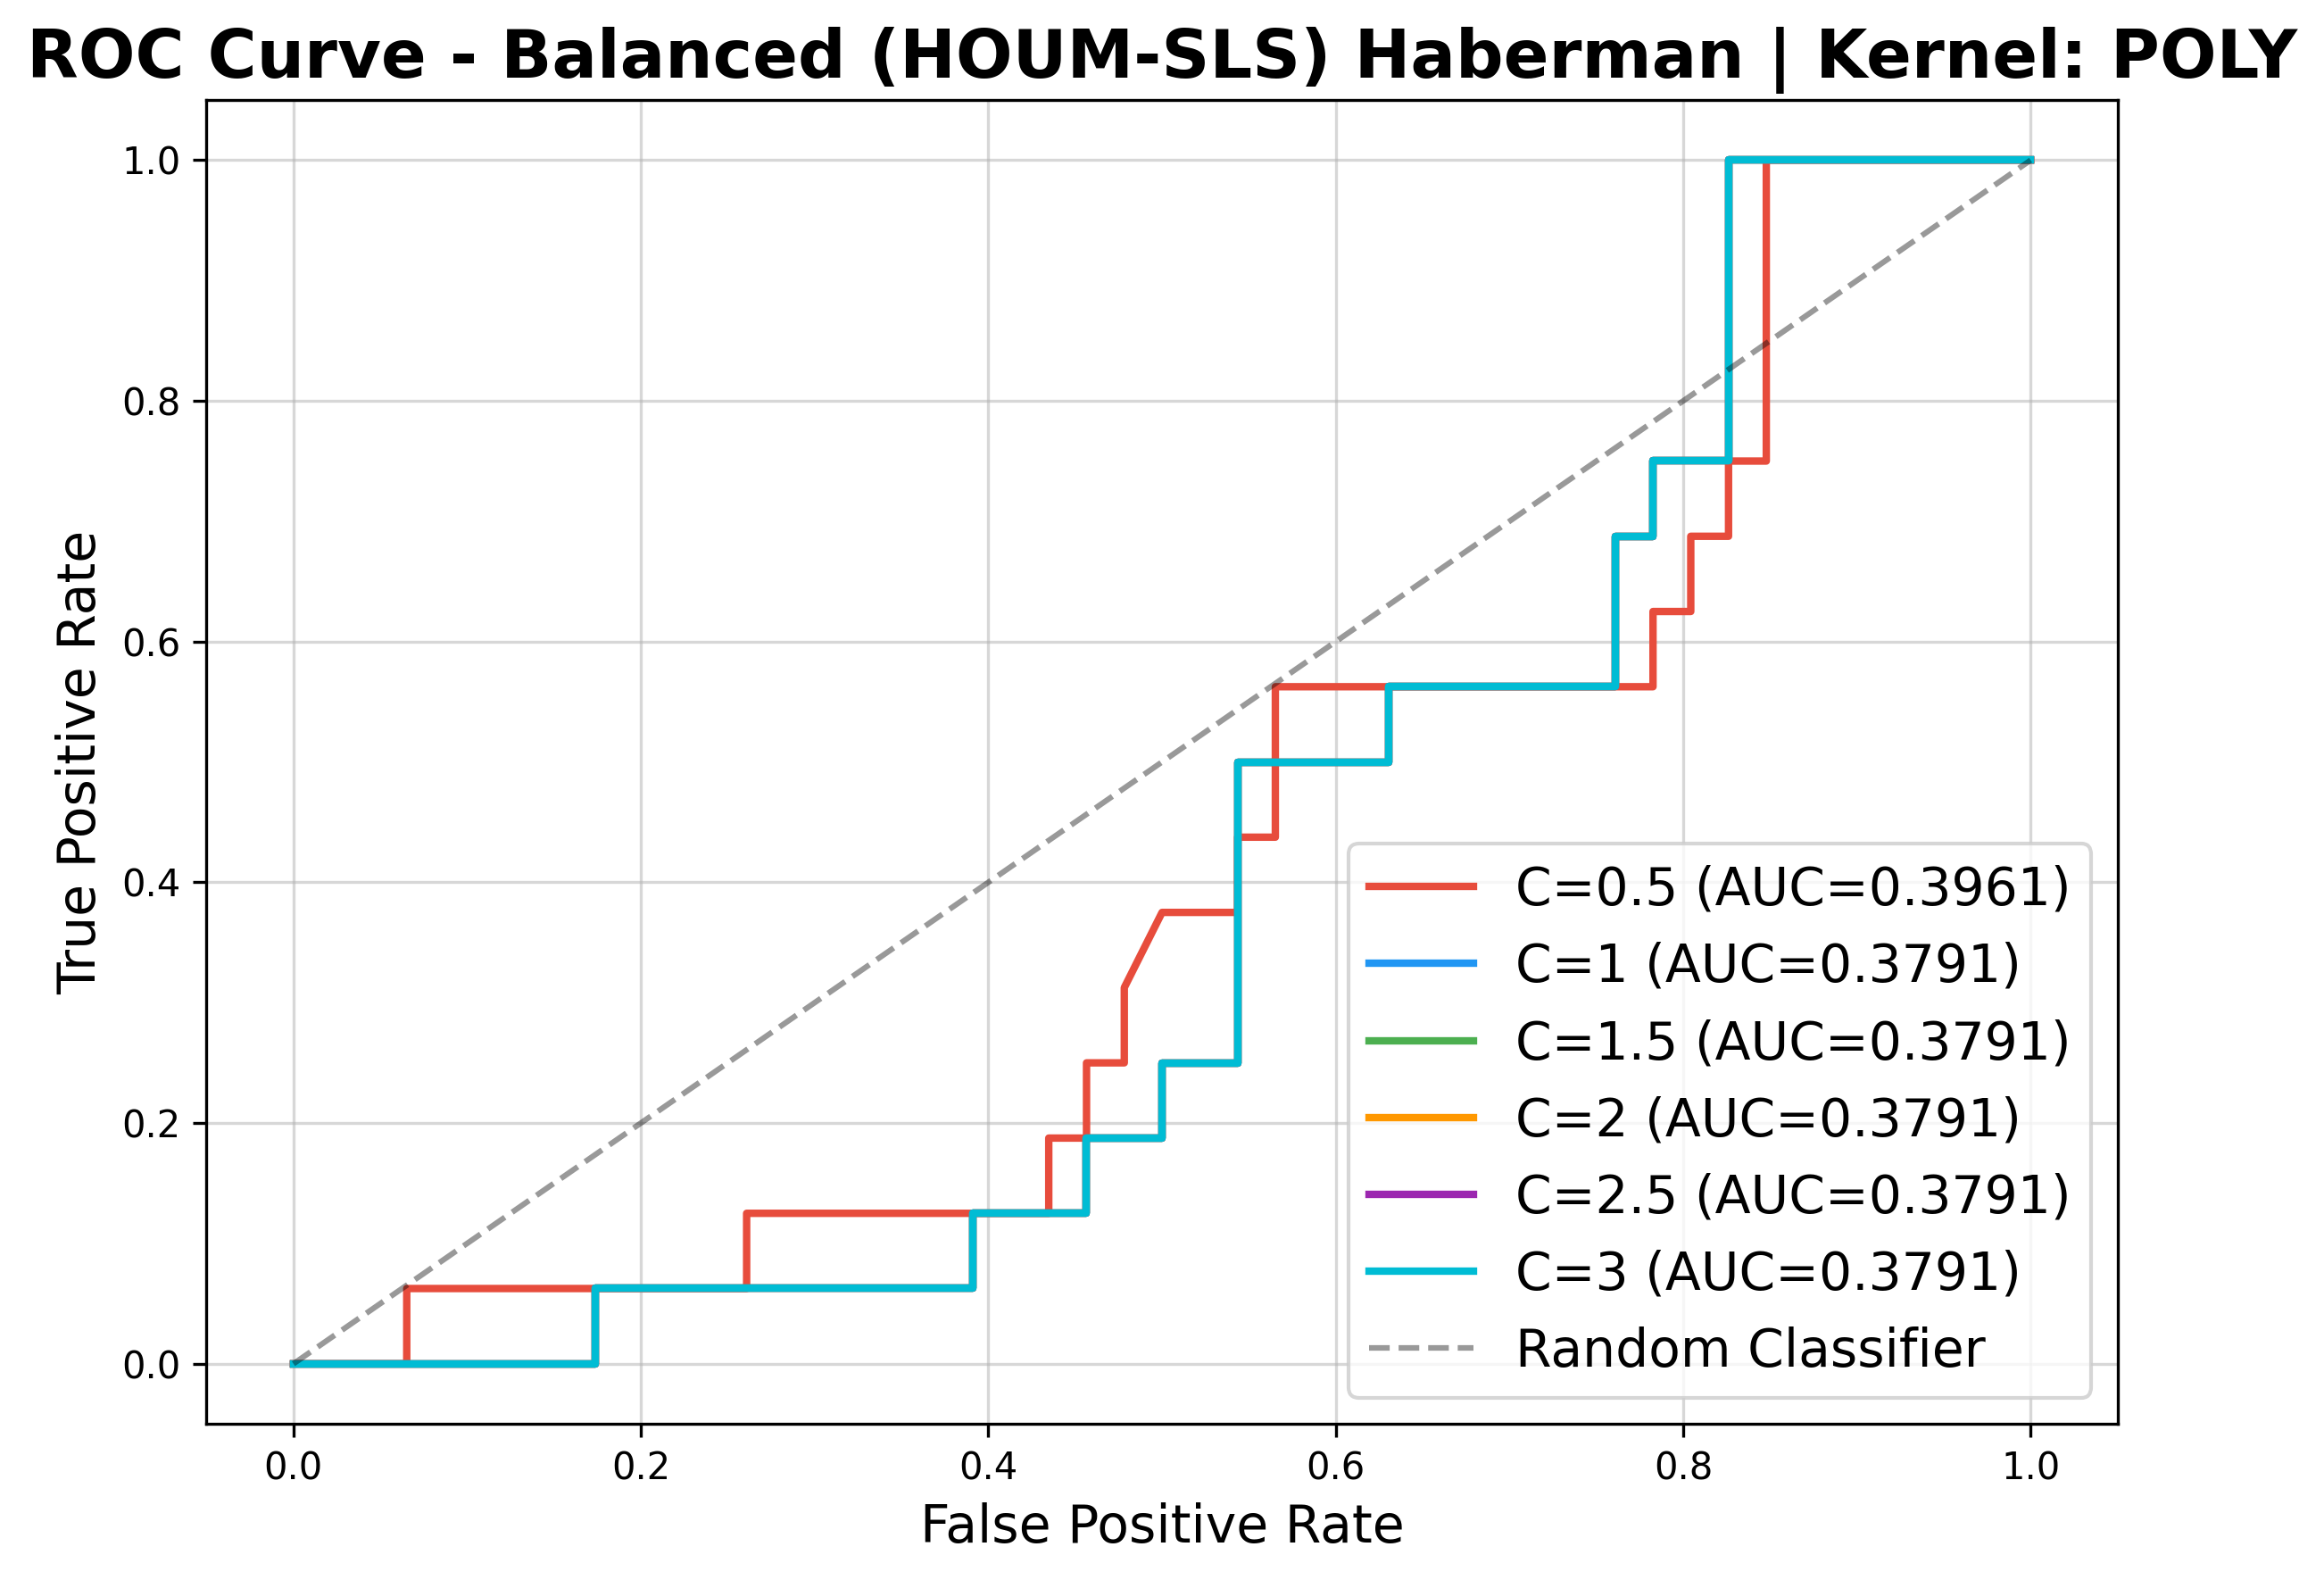
\includegraphics[width=\textwidth]{figure/roc_balanced_haberman_sls_kernel_poly.png}
        \caption{Kernel Polynomial}
        \label{fig:4.roc_sls_haberman_poly}
    \end{subfigure}
    \caption{Kurva ROC HOUM-SLSMOTE pada Dataset Haberman}
    \label{fig:4.roc_sls_haberman}
\end{figure}

Berdasarkan Tabel \ref{table:4.sls_haberman}, ROC-AUC tertinggi dicapai oleh kernel RBF dengan $C$ = 1,5 sebesar 0,6223, sedangkan \textit{Recall} (0,3750) dan G-Mean (0,4778) tertinggi diperoleh oleh kernel Linear pada $C$ = 0,5; 2; 2,5; dan 3. Kernel Linear menunjukkan konsistensi yang memadai, sedangkan kernel RBF berfluktuasi dan kernel Polynomial mencatat ROC-AUC di bawah 0,40. Dibandingkan \textit{baseline}, \textit{Recall} naik dari 0,1250 menjadi 0,3750, namun capaian ini masih terbatas akibat tumpang tindih (\textit{overlap}) antar kelas pada dataset dengan tiga fitur. \par

\subsubsection{Dataset Transfusion} \label{IV.SLS_Transfusion}
Hasil klasifikasi HOUM-SLSMOTE pada dataset Transfusion untuk seluruh kombinasi kernel dan nilai $C$ ditunjukkan pada Tabel \ref{table:4.sls_transfusion}.

\begin{table}[H]
\centering
\caption{Hasil HOUM-SLSMOTE pada Dataset Transfusion}
\label{table:4.sls_transfusion}
\footnotesize
\begin{tabular}{|l|c|c|c|c|c|c|}
\hline
\textbf{No} & \textbf{Kernel} & \textbf{C} & \textbf{ROC-AUC} & \textbf{\textit{Recall}} & \textbf{\textit{Precision}} & \textbf{G-Mean} \\
\hline
1 & Linear & 0,5 & 0,6821 & 0,7222 & 0,3939 & 0,6847 \\
\hline
2 & Linear & 1 & 0,7199 & 0,7222 & 0,3939 & 0,6847 \\
\hline
3 & Linear & 1,5 & 0,7167 & 0,6944 & 0,3676 & 0,6577 \\
\hline
4 & Linear & 2 & 0,7197 & 0,7500 & \textbf{0,4030} & \textbf{0,6977} \\
\hline
5 & Linear & 2,5 & 0,6943 & \textbf{0,7778} & 0,3836 & 0,6861 \\
\hline
6 & Linear & 3 & 0,6825 & 0,6667 & 0,3582 & 0,6444 \\
\hline
7 & RBF & 0,5 & 0,7024 & 0,7222 & 0,4000 & 0,6893 \\
\hline
8 & RBF & 1 & 0,6933 & 0,6111 & 0,3667 & 0,6383 \\
\hline
9 & RBF & 1,5 & 0,7019 & 0,6111 & 0,3929 & 0,6549 \\
\hline
10 & RBF & 2 & 0,7139 & 0,5833 & 0,3889 & 0,6438 \\
\hline
11 & RBF & 2,5 & \textbf{0,7267} & 0,6111 & 0,3729 & 0,6425 \\
\hline
12 & RBF & 3 & 0,7102 & 0,6111 & 0,4000 & 0,6589 \\
\hline
13 & Poly & 0,5 & 0,6686 & 0,5000 & 0,3158 & 0,5735 \\
\hline
14 & Poly & 1 & 0,7098 & 0,6111 & 0,3607 & 0,6341 \\
\hline
15 & Poly & 1,5 & 0,6884 & 0,6389 & 0,3194 & 0,6036 \\
\hline
16 & Poly & 2 & 0,7091 & 0,6111 & 0,3729 & 0,6425 \\
\hline
17 & Poly & 2,5 & 0,6801 & 0,5556 & 0,3636 & 0,6205 \\
\hline
18 & Poly & 3 & 0,6988 & 0,5833 & 0,3559 & 0,6236 \\
\hline
\end{tabular}
\end{table}

Kurva ROC untuk masing-masing kernel pada dataset Transfusion ditunjukkan pada Gambar \ref{fig:4.roc_sls_transfusion}.

\begin{figure}[H]
    \centering
    \begin{subfigure}[b]{0.47\textwidth}
        \centering
        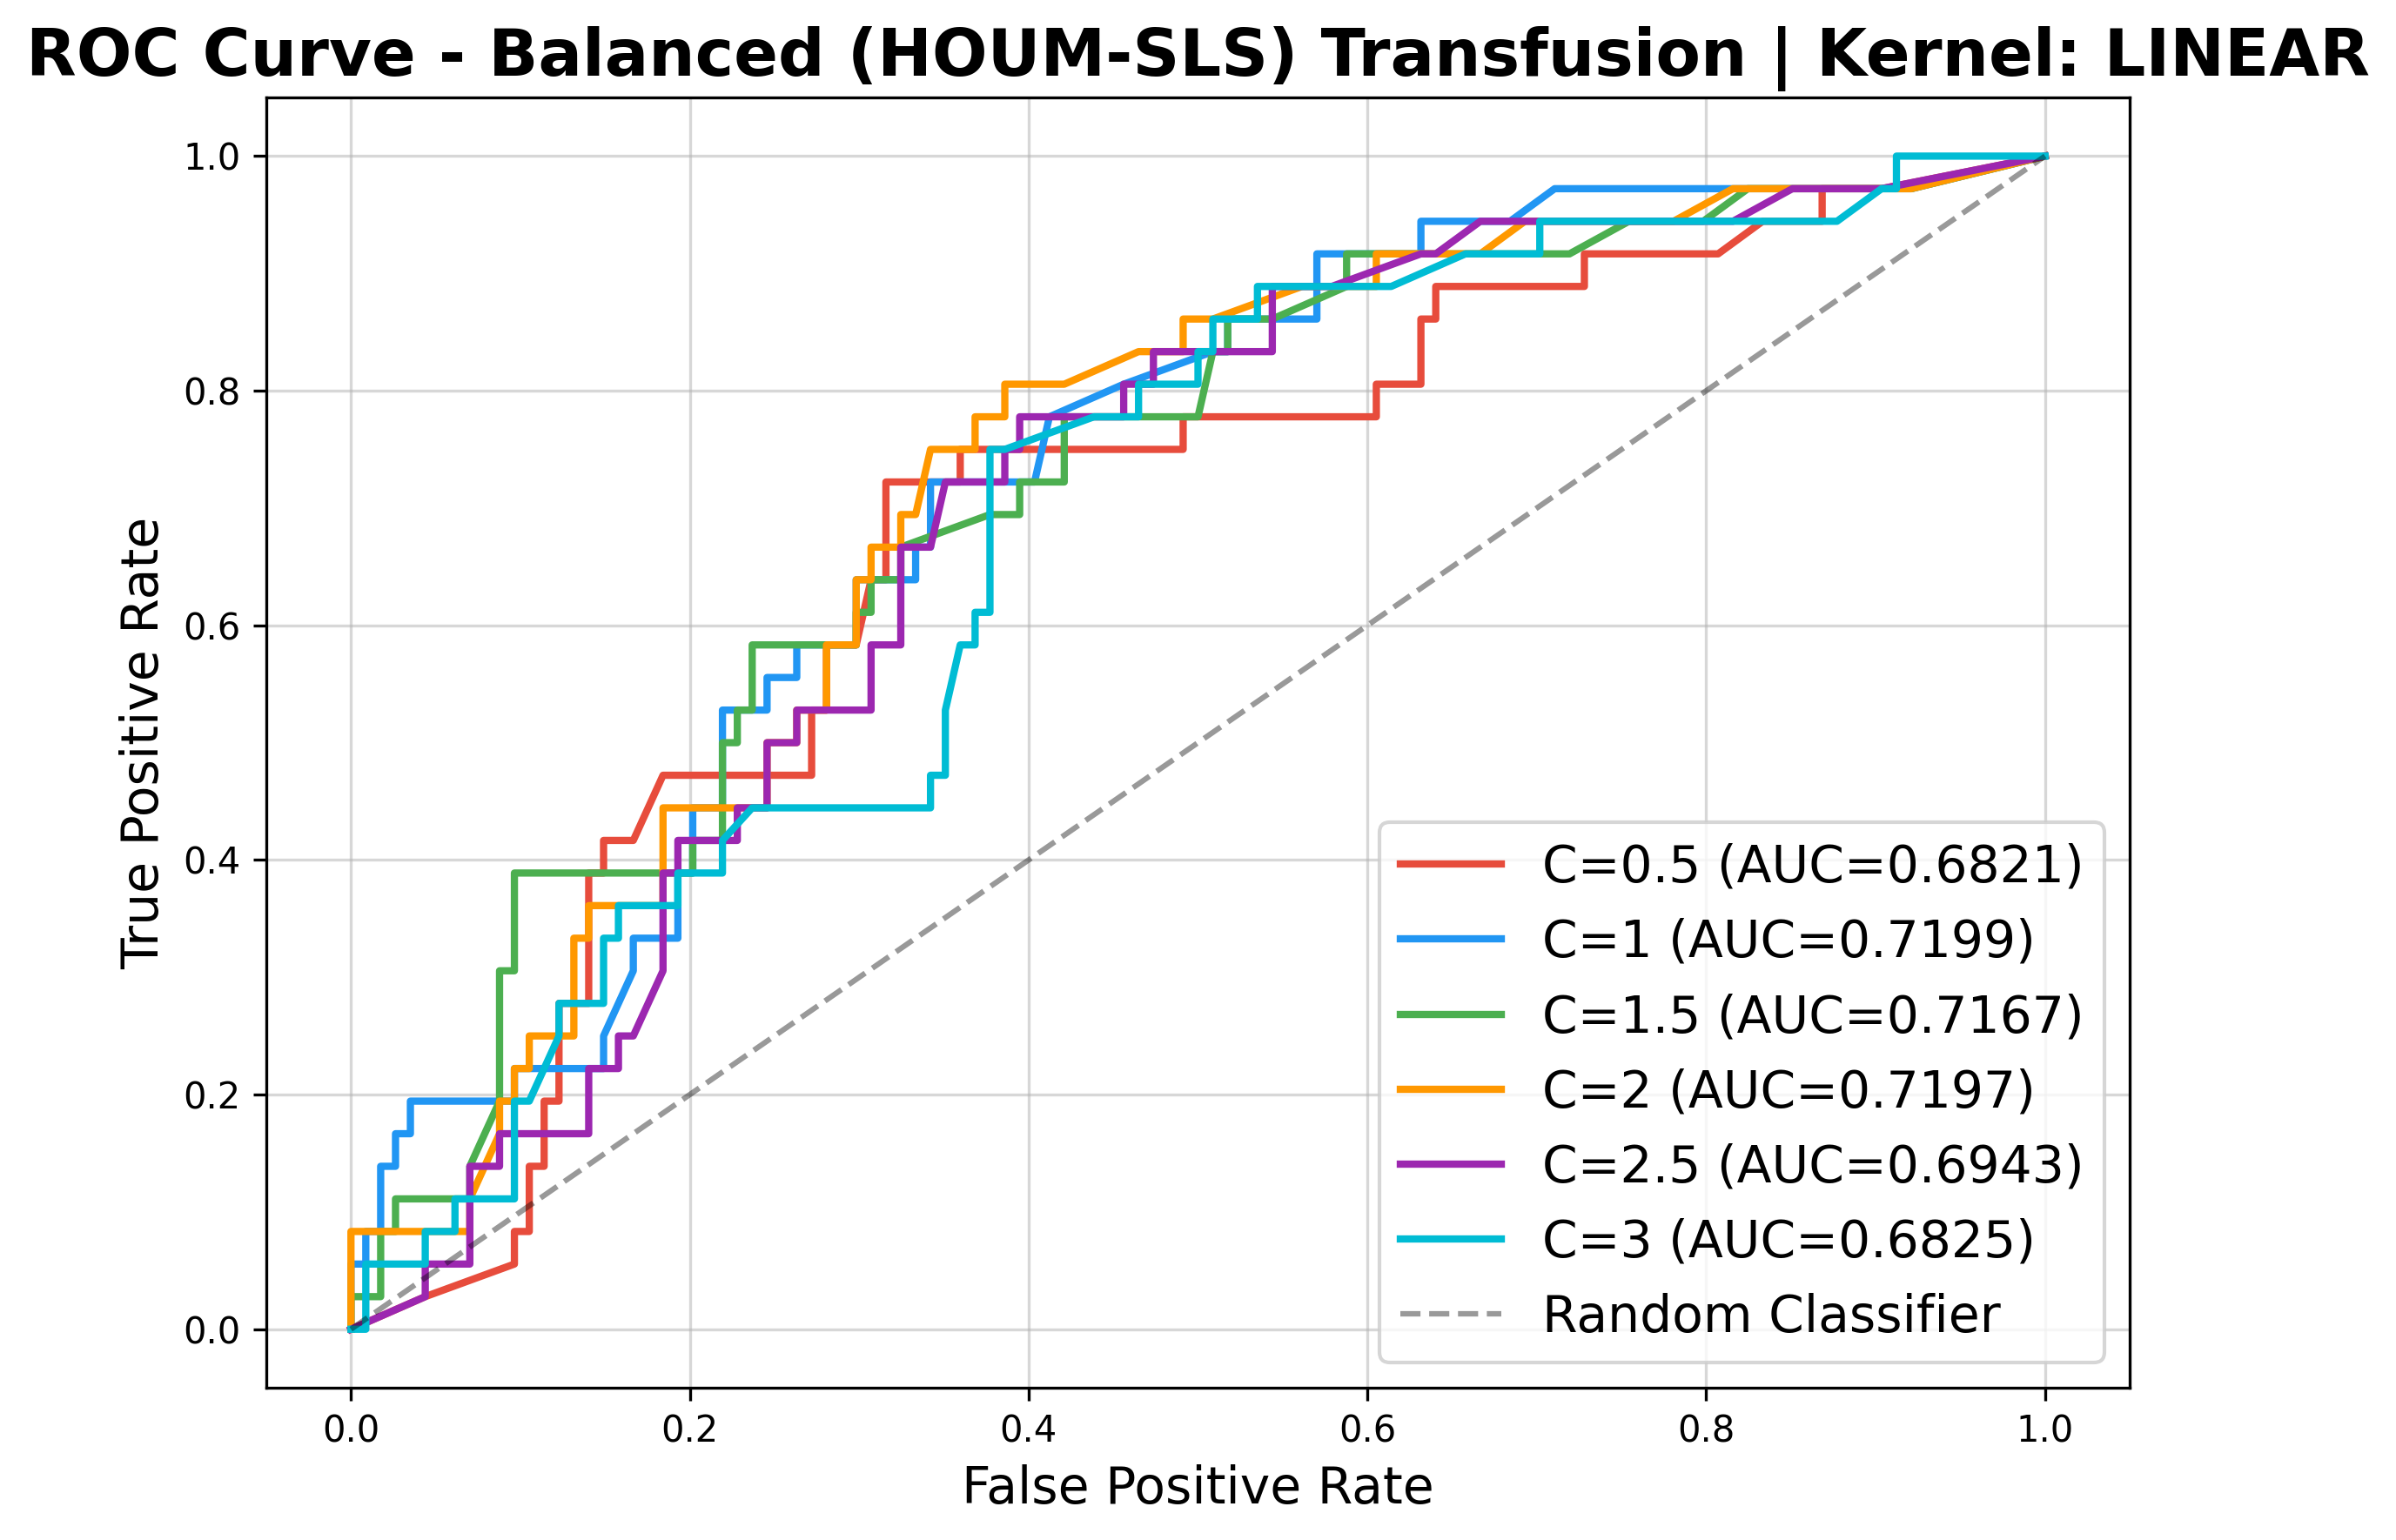
\includegraphics[width=\textwidth]{figure/roc_balanced_transfusion_sls_kernel_linear.png}
        \caption{Kernel Linear}
        \label{fig:4.roc_sls_transfusion_linear}
    \end{subfigure}
    \hfill
    \begin{subfigure}[b]{0.47\textwidth}
        \centering
        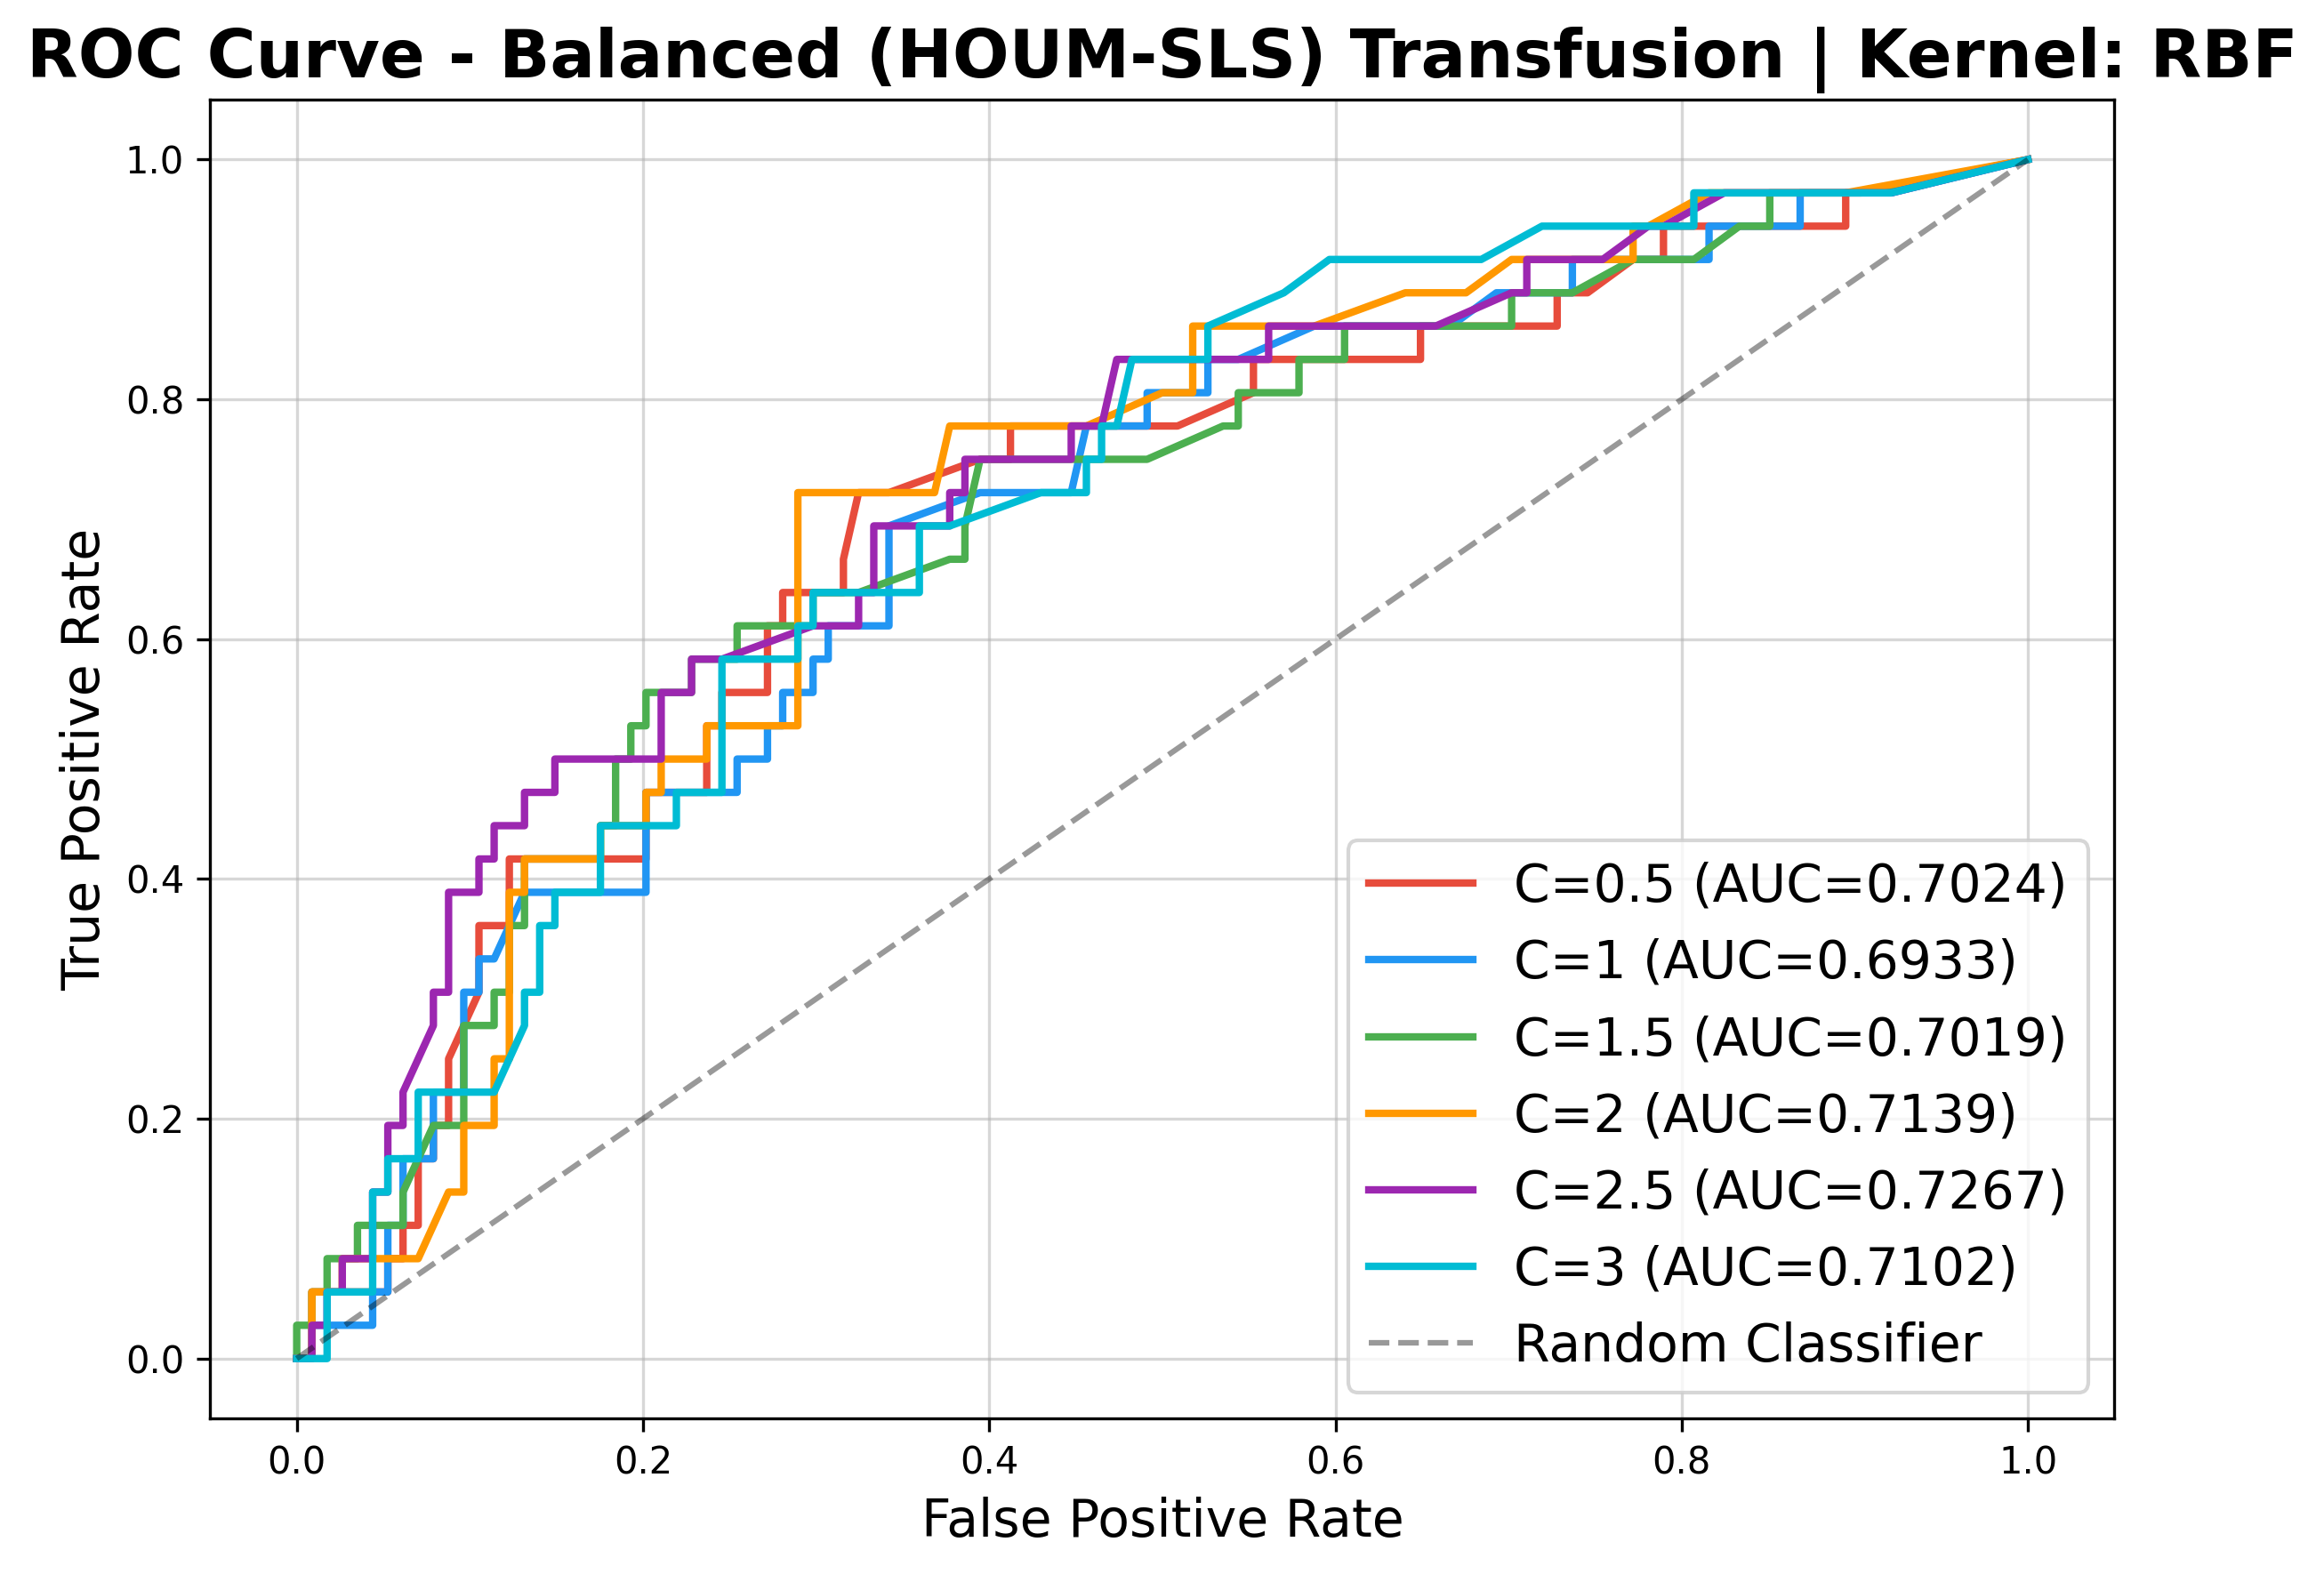
\includegraphics[width=\textwidth]{figure/roc_balanced_transfusion_sls_kernel_rbf.png}
        \caption{Kernel RBF}
        \label{fig:4.roc_sls_transfusion_rbf}
    \end{subfigure}

    \vspace{0.5em}

    \begin{subfigure}[b]{0.47\textwidth}
        \centering
        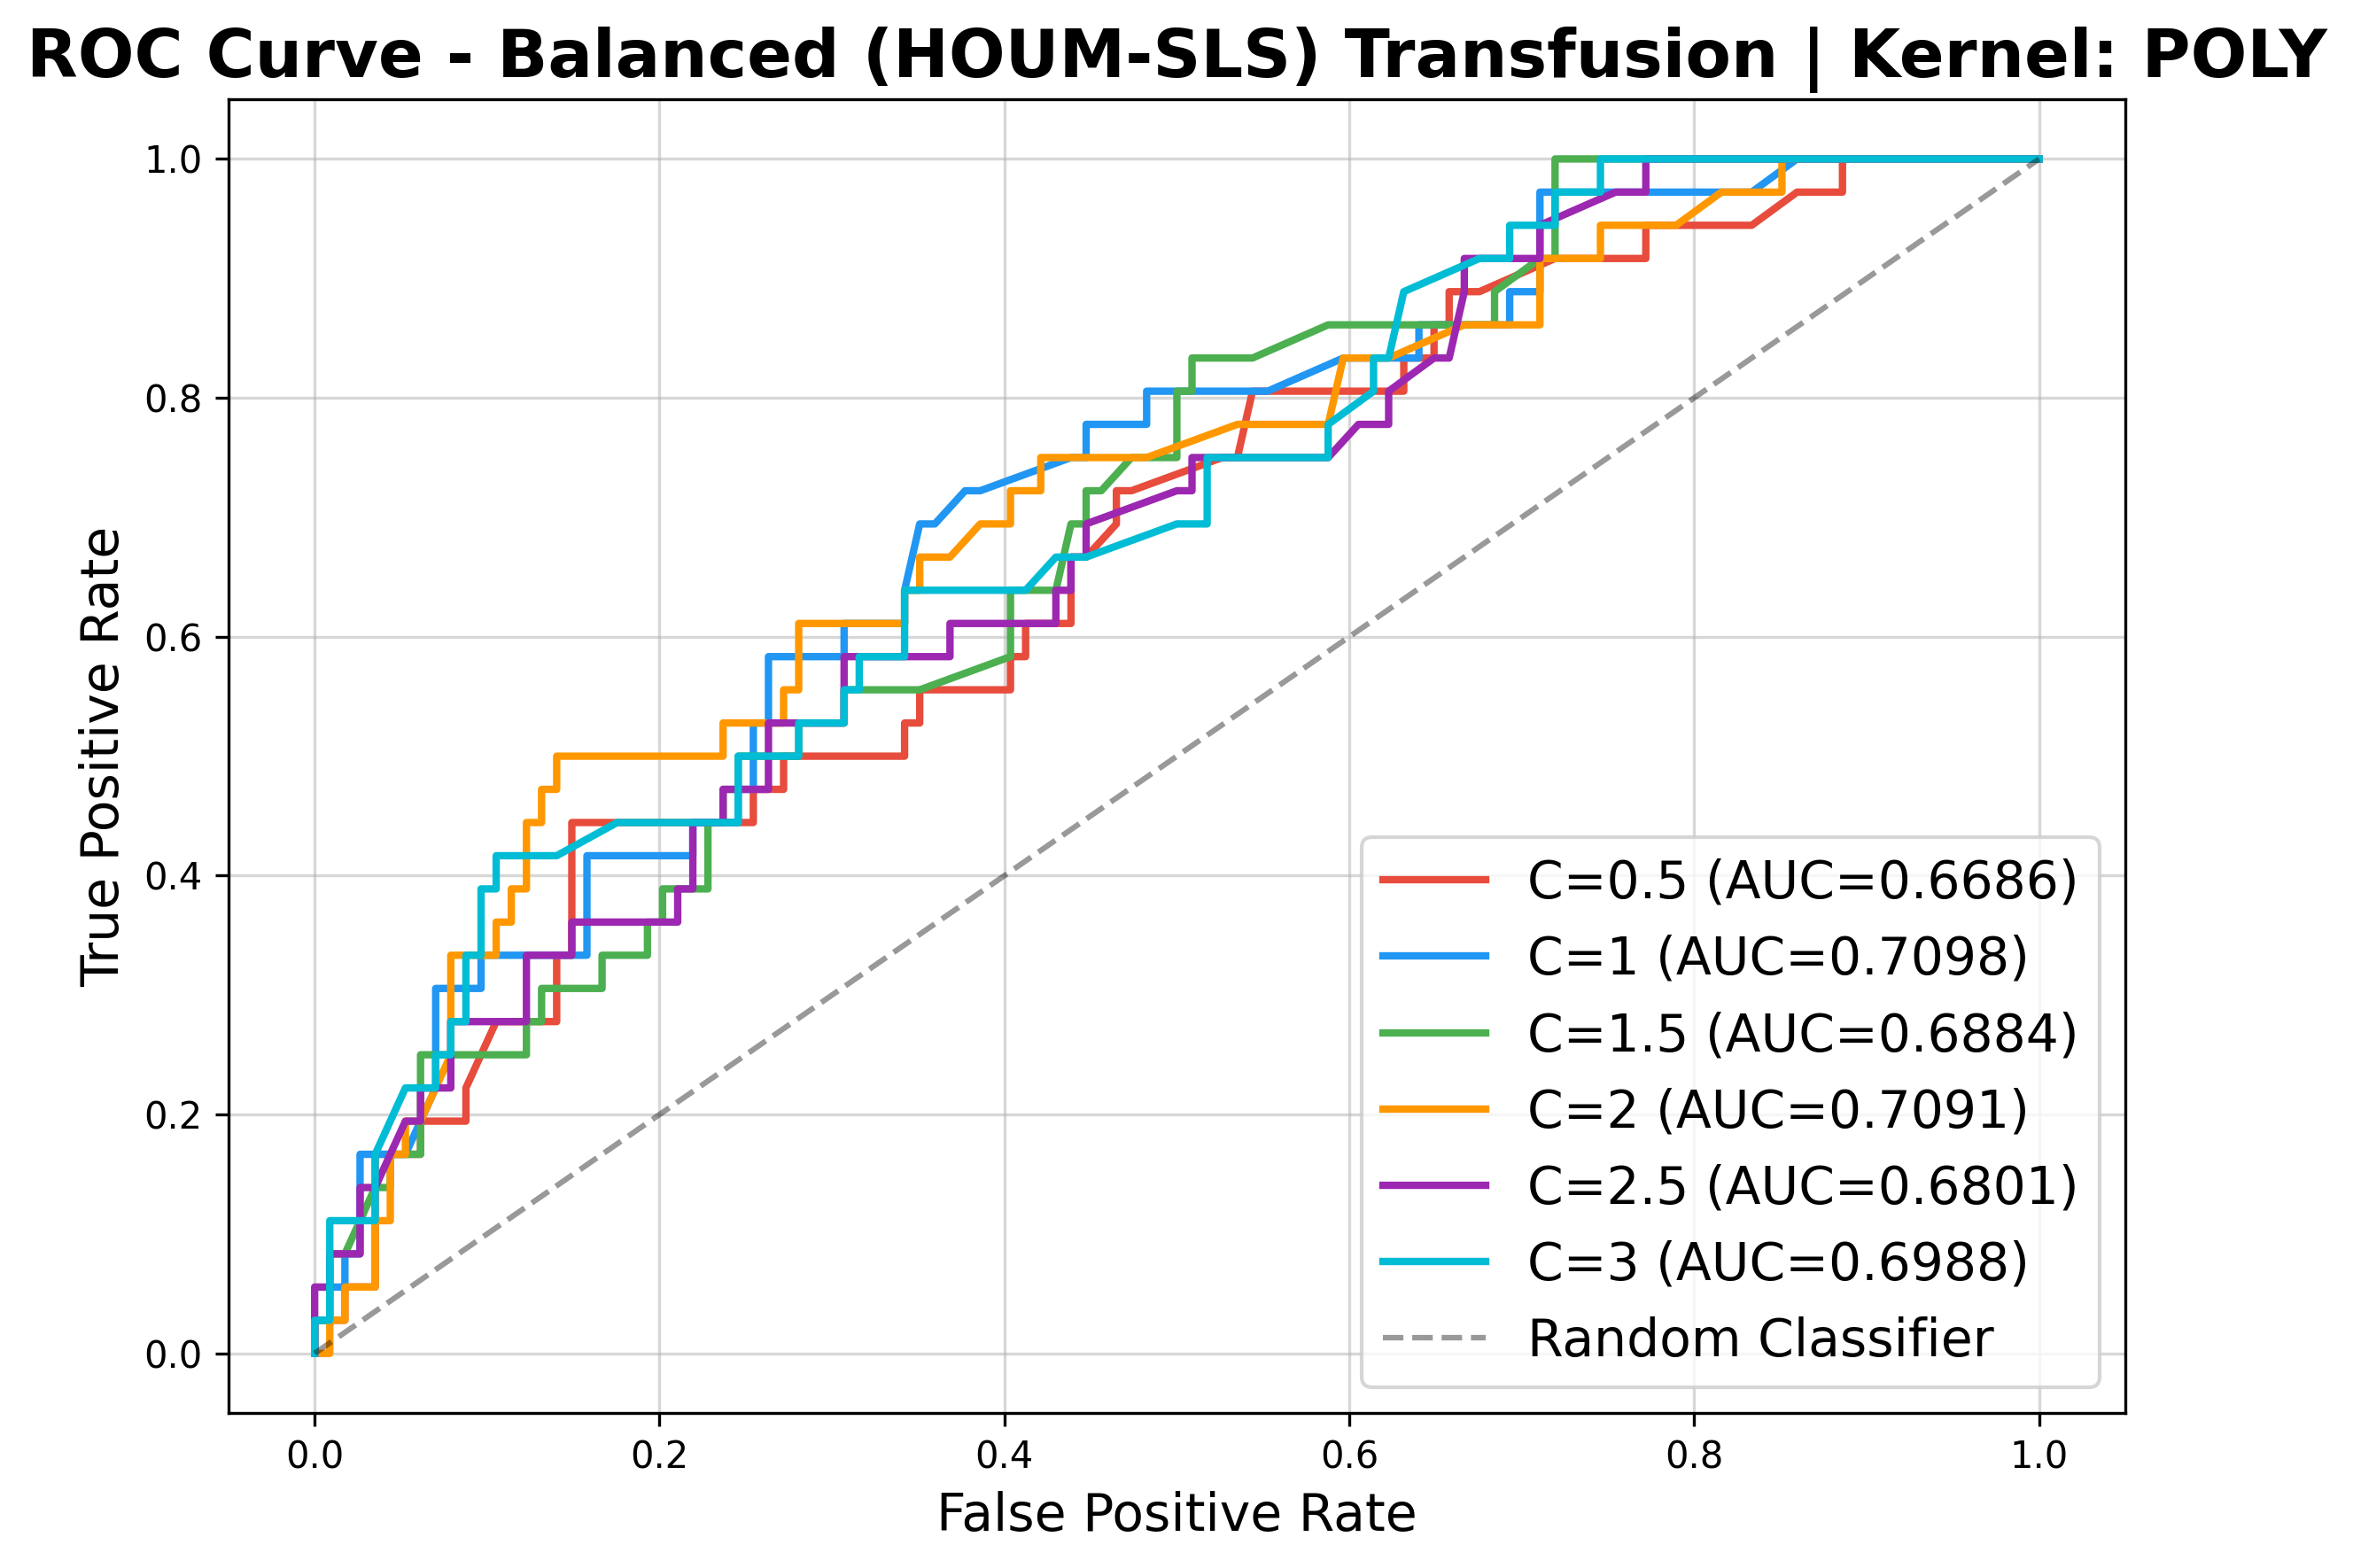
\includegraphics[width=\textwidth]{figure/roc_balanced_transfusion_sls_kernel_poly.png}
        \caption{Kernel Polynomial}
        \label{fig:4.roc_sls_transfusion_poly}
    \end{subfigure}
    \caption{Kurva ROC HOUM-SLSMOTE pada Dataset Transfusion}
    \label{fig:4.roc_sls_transfusion}
\end{figure}

Berdasarkan Tabel \ref{table:4.sls_transfusion}, nilai \textit{Recall} tertinggi sebesar 0,7778 dicapai oleh kernel Linear dengan $C$ = 2,5. Nilai ROC-AUC tertinggi diperoleh oleh kernel RBF dengan $C$ = 2,5 sebesar 0,7267, sedangkan G-Mean tertinggi sebesar 0,6977 dan \textit{Precision} tertinggi sebesar 0,4030 secara bersamaan dicapai oleh kernel Linear dengan $C$ = 2. Kernel Linear mendominasi performa pada dataset ini karena memberikan hasil yang lebih seimbang antara \textit{Recall} dan \textit{Precision}, sedangkan kernel Polynomial mencatat performa paling rendah pada seluruh metrik evaluasi.

\subsubsection{Dataset Glass5} \label{IV.SLS_Glass}
Hasil klasifikasi HOUM-SLSMOTE pada dataset Glass5 untuk seluruh kombinasi kernel dan nilai $C$ ditunjukkan pada Tabel \ref{table:4.sls_glass}.

\begin{table}[H]
\centering
\caption{Hasil HOUM-SLSMOTE pada Dataset Glass5}
\label{table:4.sls_glass}
\footnotesize
\begin{tabular}{|l|c|c|c|c|c|c|}
\hline
\textbf{No} & \textbf{Kernel} & \textbf{C} & \textbf{ROC-AUC} & \textbf{\textit{Recall}} & \textbf{\textit{Precision}} & \textbf{G-Mean} \\
\hline
1 & Linear & 0,5 & \textbf{0,9878} & \textbf{1,0000} & \textbf{0,5000} & \textbf{0,9753} \\
\hline
2 & Linear & 1 & \textbf{0,9878} & \textbf{1,0000} & \textbf{0,5000} & \textbf{0,9753} \\
\hline
3 & Linear & 1,5 & \textbf{0,9878} & \textbf{1,0000} & \textbf{0,5000} & \textbf{0,9753} \\
\hline
4 & Linear & 2 & \textbf{0,9878} & \textbf{1,0000} & \textbf{0,5000} & \textbf{0,9753} \\
\hline
5 & Linear & 2,5 & \textbf{0,9878} & \textbf{1,0000} & \textbf{0,5000} & \textbf{0,9753} \\
\hline
6 & Linear & 3 & \textbf{0,9878} & \textbf{1,0000} & \textbf{0,5000} & \textbf{0,9753} \\
\hline
7 & RBF & 0,5 & \textbf{0,9878} & \textbf{1,0000} & 0,4000 & 0,9627 \\
\hline
8 & RBF & 1 & \textbf{0,9878} & \textbf{1,0000} & 0,4000 & 0,9627 \\
\hline
9 & RBF & 1,5 & \textbf{0,9878} & \textbf{1,0000} & 0,4000 & 0,9627 \\
\hline
10 & RBF & 2 & \textbf{0,9878} & \textbf{1,0000} & 0,4000 & 0,9627 \\
\hline
11 & RBF & 2,5 & \textbf{0,9878} & \textbf{1,0000} & 0,4000 & 0,9627 \\
\hline
12 & RBF & 3 & \textbf{0,9878} & \textbf{1,0000} & 0,4000 & 0,9627 \\
\hline
13 & Poly & 0,5 & \textbf{0,9878} & \textbf{1,0000} & \textbf{0,5000} & \textbf{0,9753} \\
\hline
14 & Poly & 1 & \textbf{0,9878} & \textbf{1,0000} & \textbf{0,5000} & \textbf{0,9753} \\
\hline
15 & Poly & 1,5 & 0,9756 & \textbf{1,0000} & 0,4000 & 0,9627 \\
\hline
16 & Poly & 2 & 0,9756 & \textbf{1,0000} & 0,4000 & 0,9627 \\
\hline
17 & Poly & 2,5 & 0,9756 & \textbf{1,0000} & 0,4000 & 0,9627 \\
\hline
18 & Poly & 3 & 0,9756 & \textbf{1,0000} & 0,4000 & 0,9627 \\
\hline
\end{tabular}
\end{table}

Kurva ROC untuk masing-masing kernel pada dataset Glass5 ditunjukkan pada Gambar \ref{fig:4.roc_sls_glass}.

\begin{figure}[H]
    \centering
    \begin{subfigure}[b]{0.47\textwidth}
        \centering
        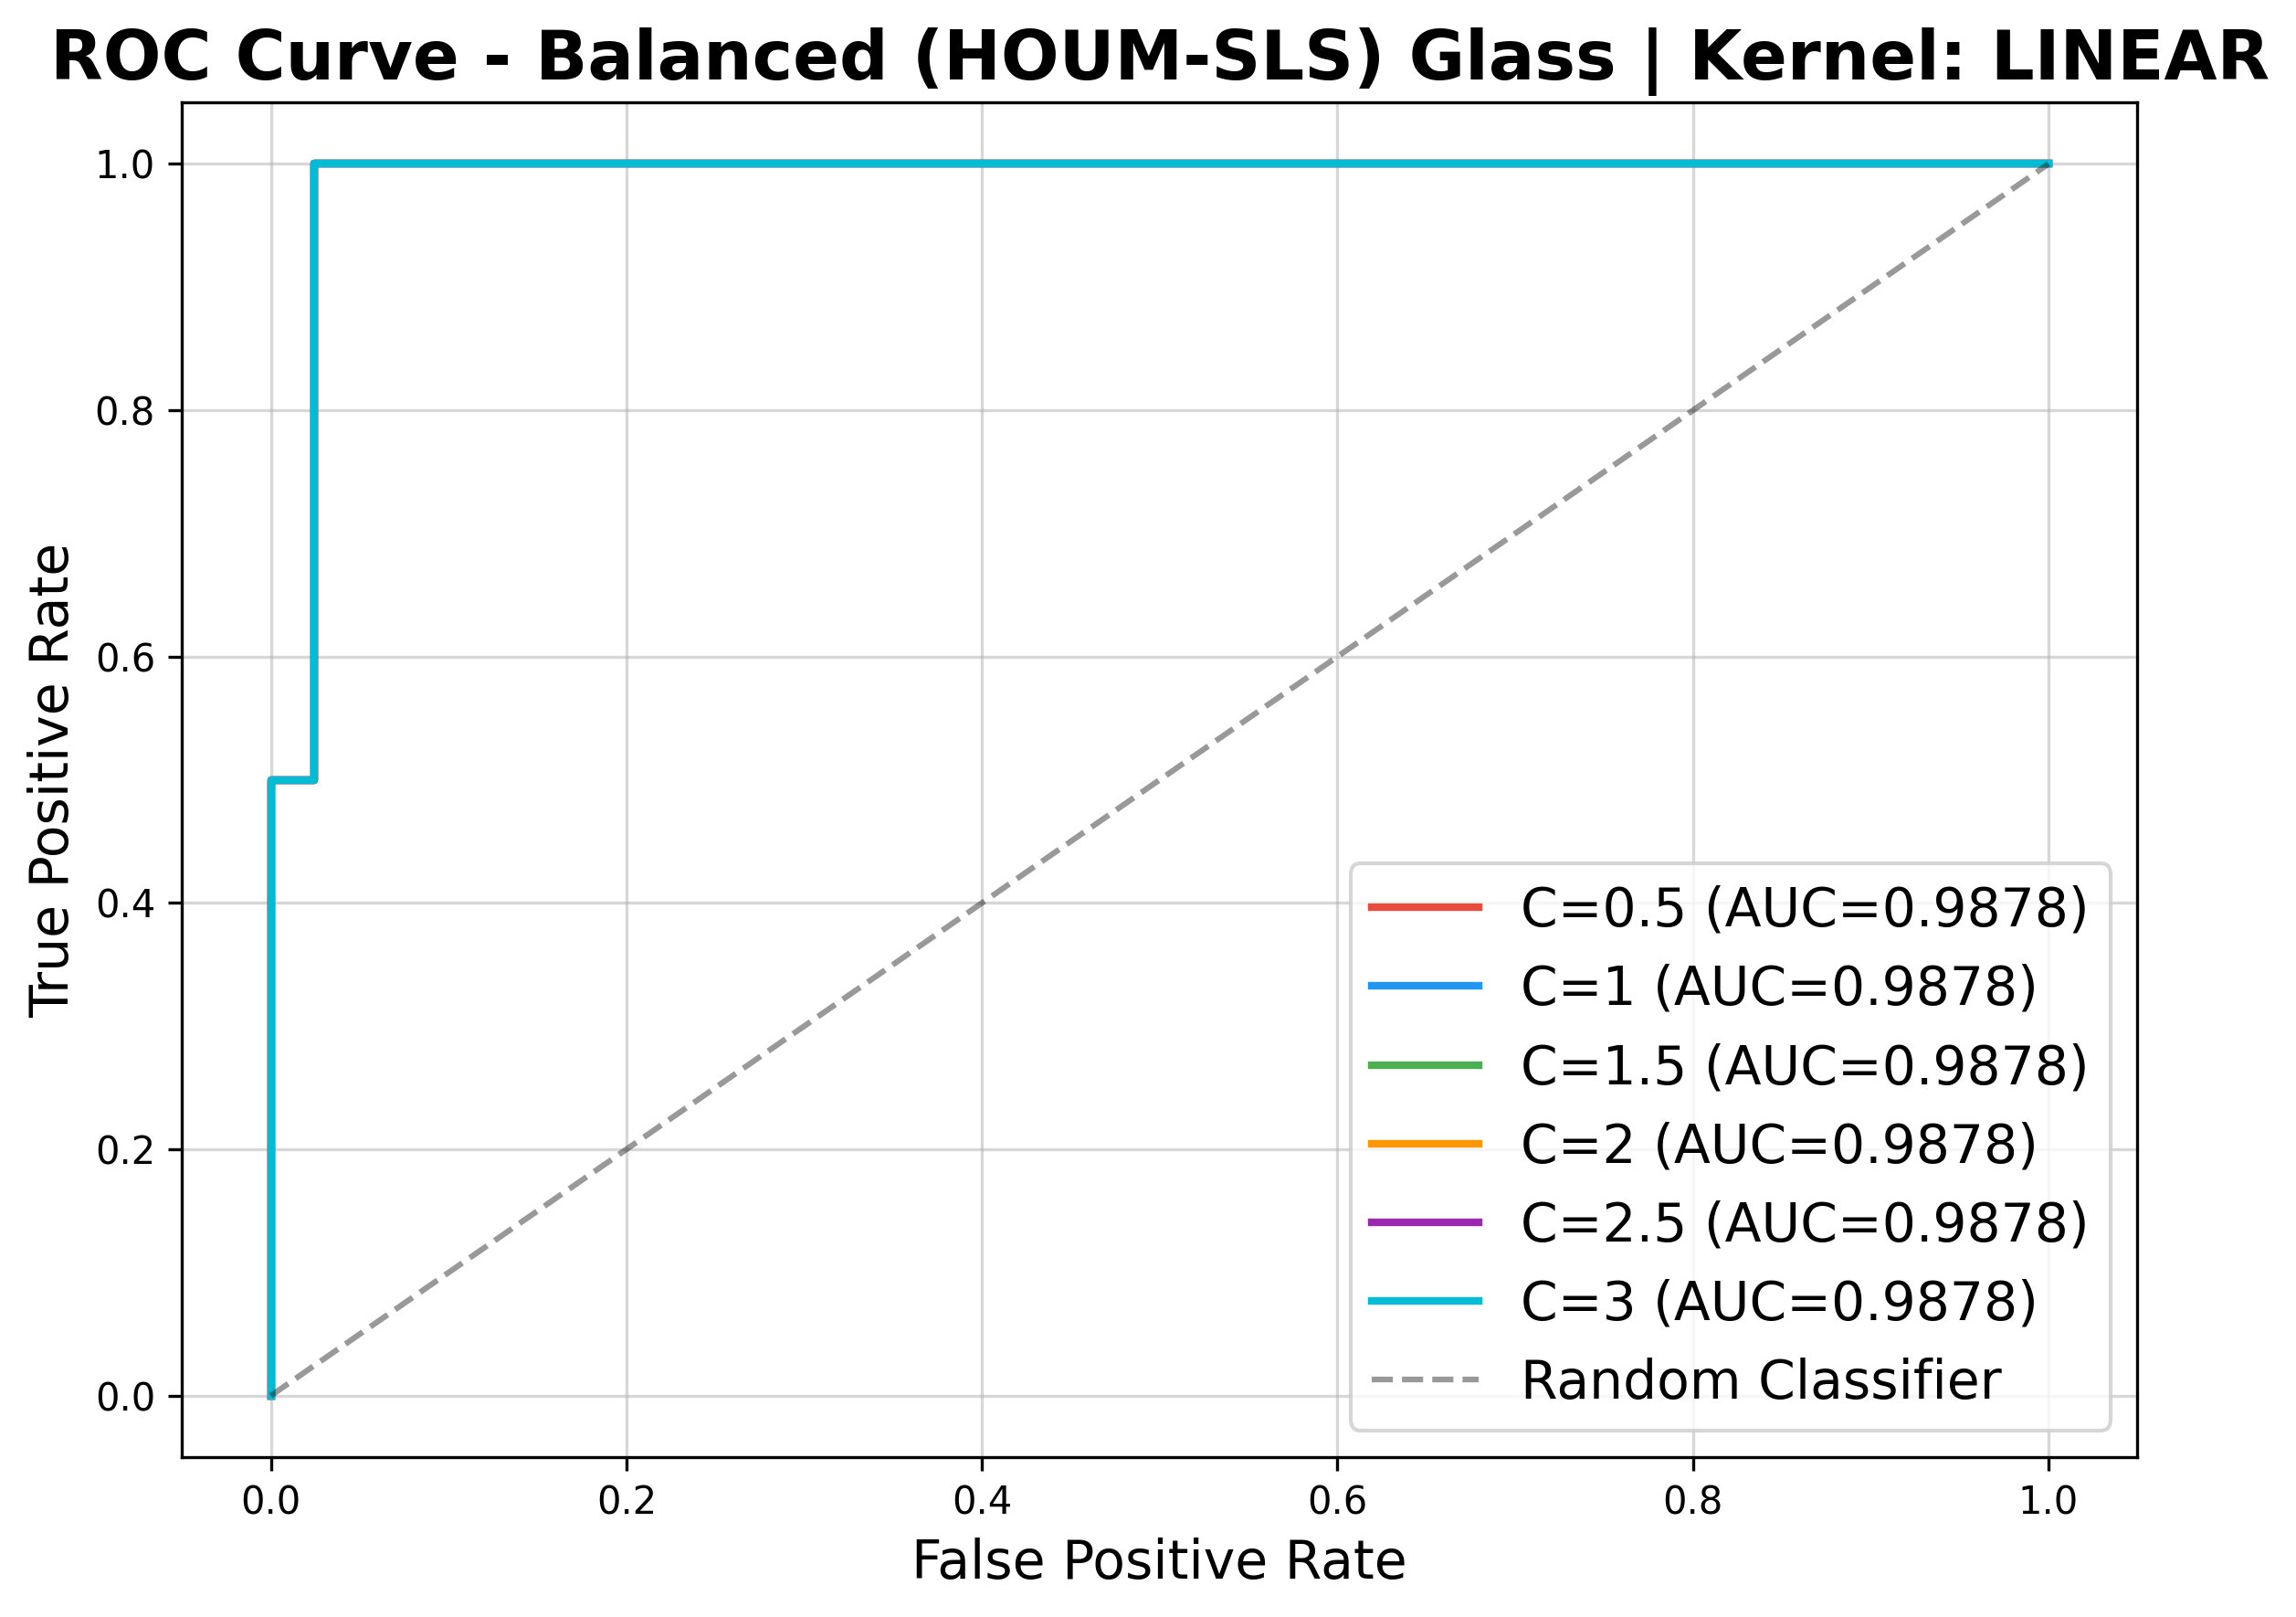
\includegraphics[width=\textwidth]{figure/roc_balanced_glass_sls_kernel_linear.png}
        \caption{Kernel Linear}
        \label{fig:4.roc_sls_glass_linear}
    \end{subfigure}
    \hfill
    \begin{subfigure}[b]{0.47\textwidth}
        \centering
        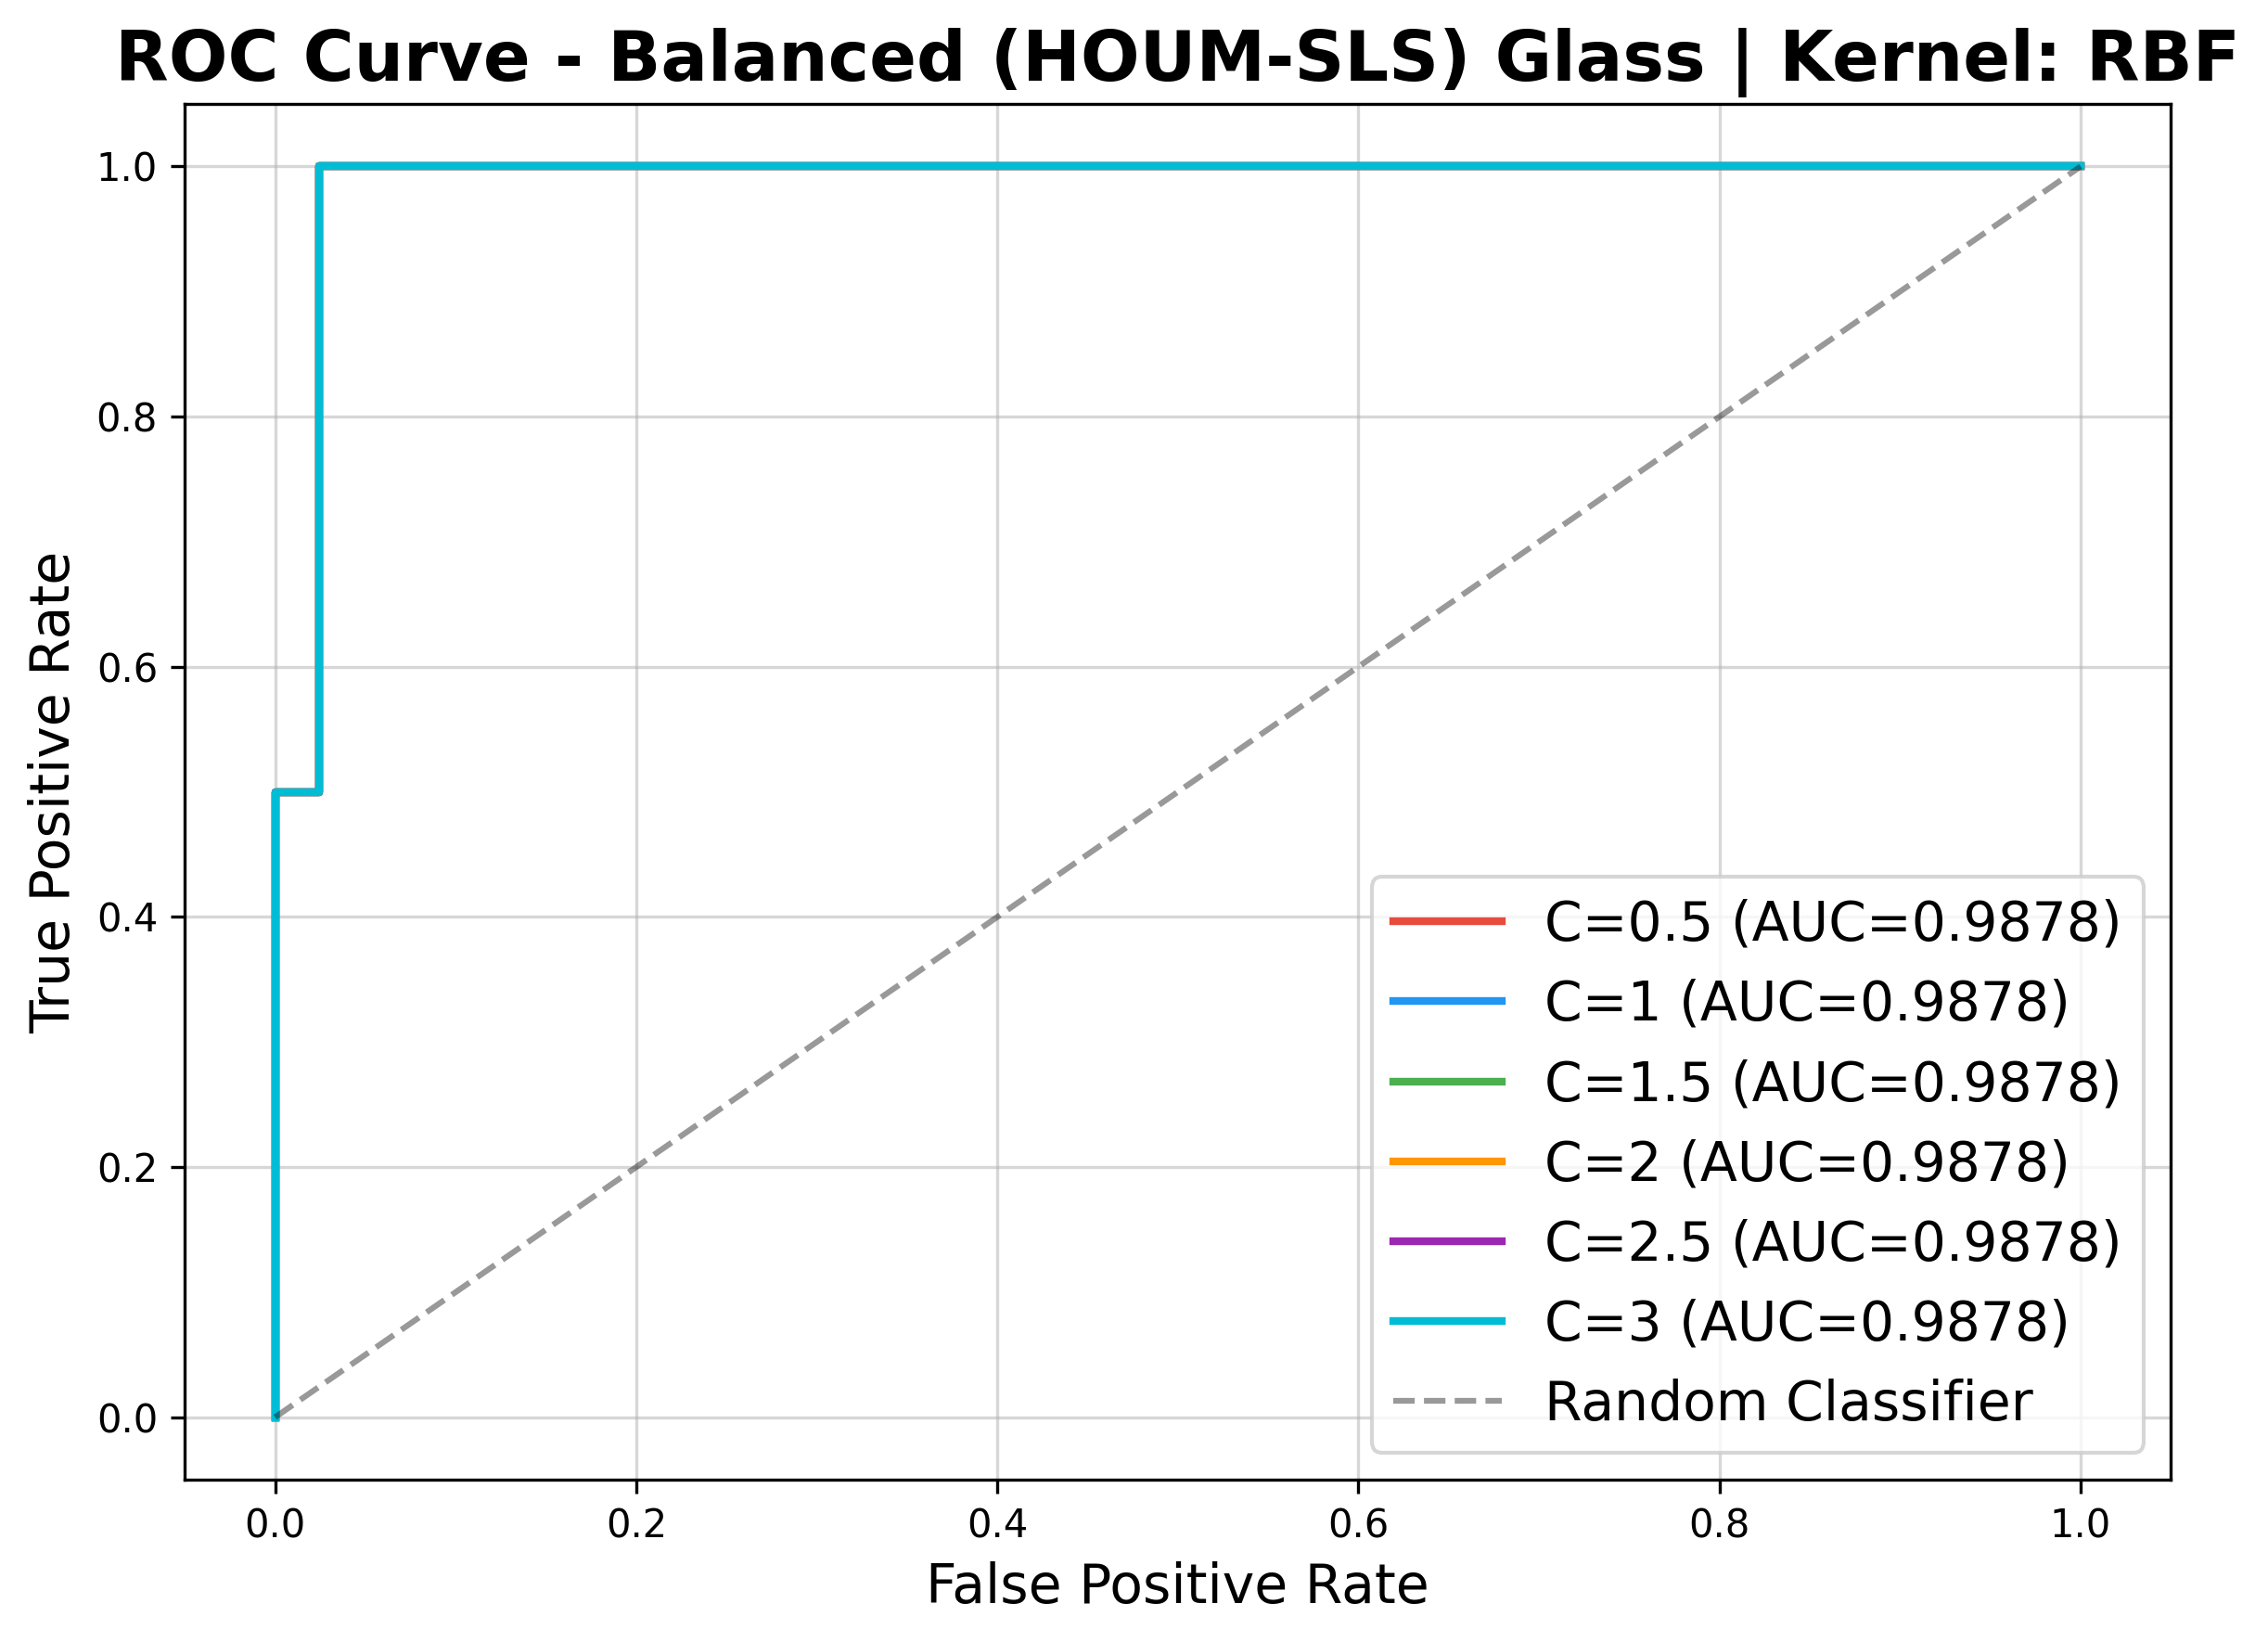
\includegraphics[width=\textwidth]{figure/roc_balanced_glass_sls_kernel_rbf.png}
        \caption{Kernel RBF}
        \label{fig:4.roc_sls_glass_rbf}
    \end{subfigure}

    \vspace{0.5em}

    \begin{subfigure}[b]{0.47\textwidth}
        \centering
        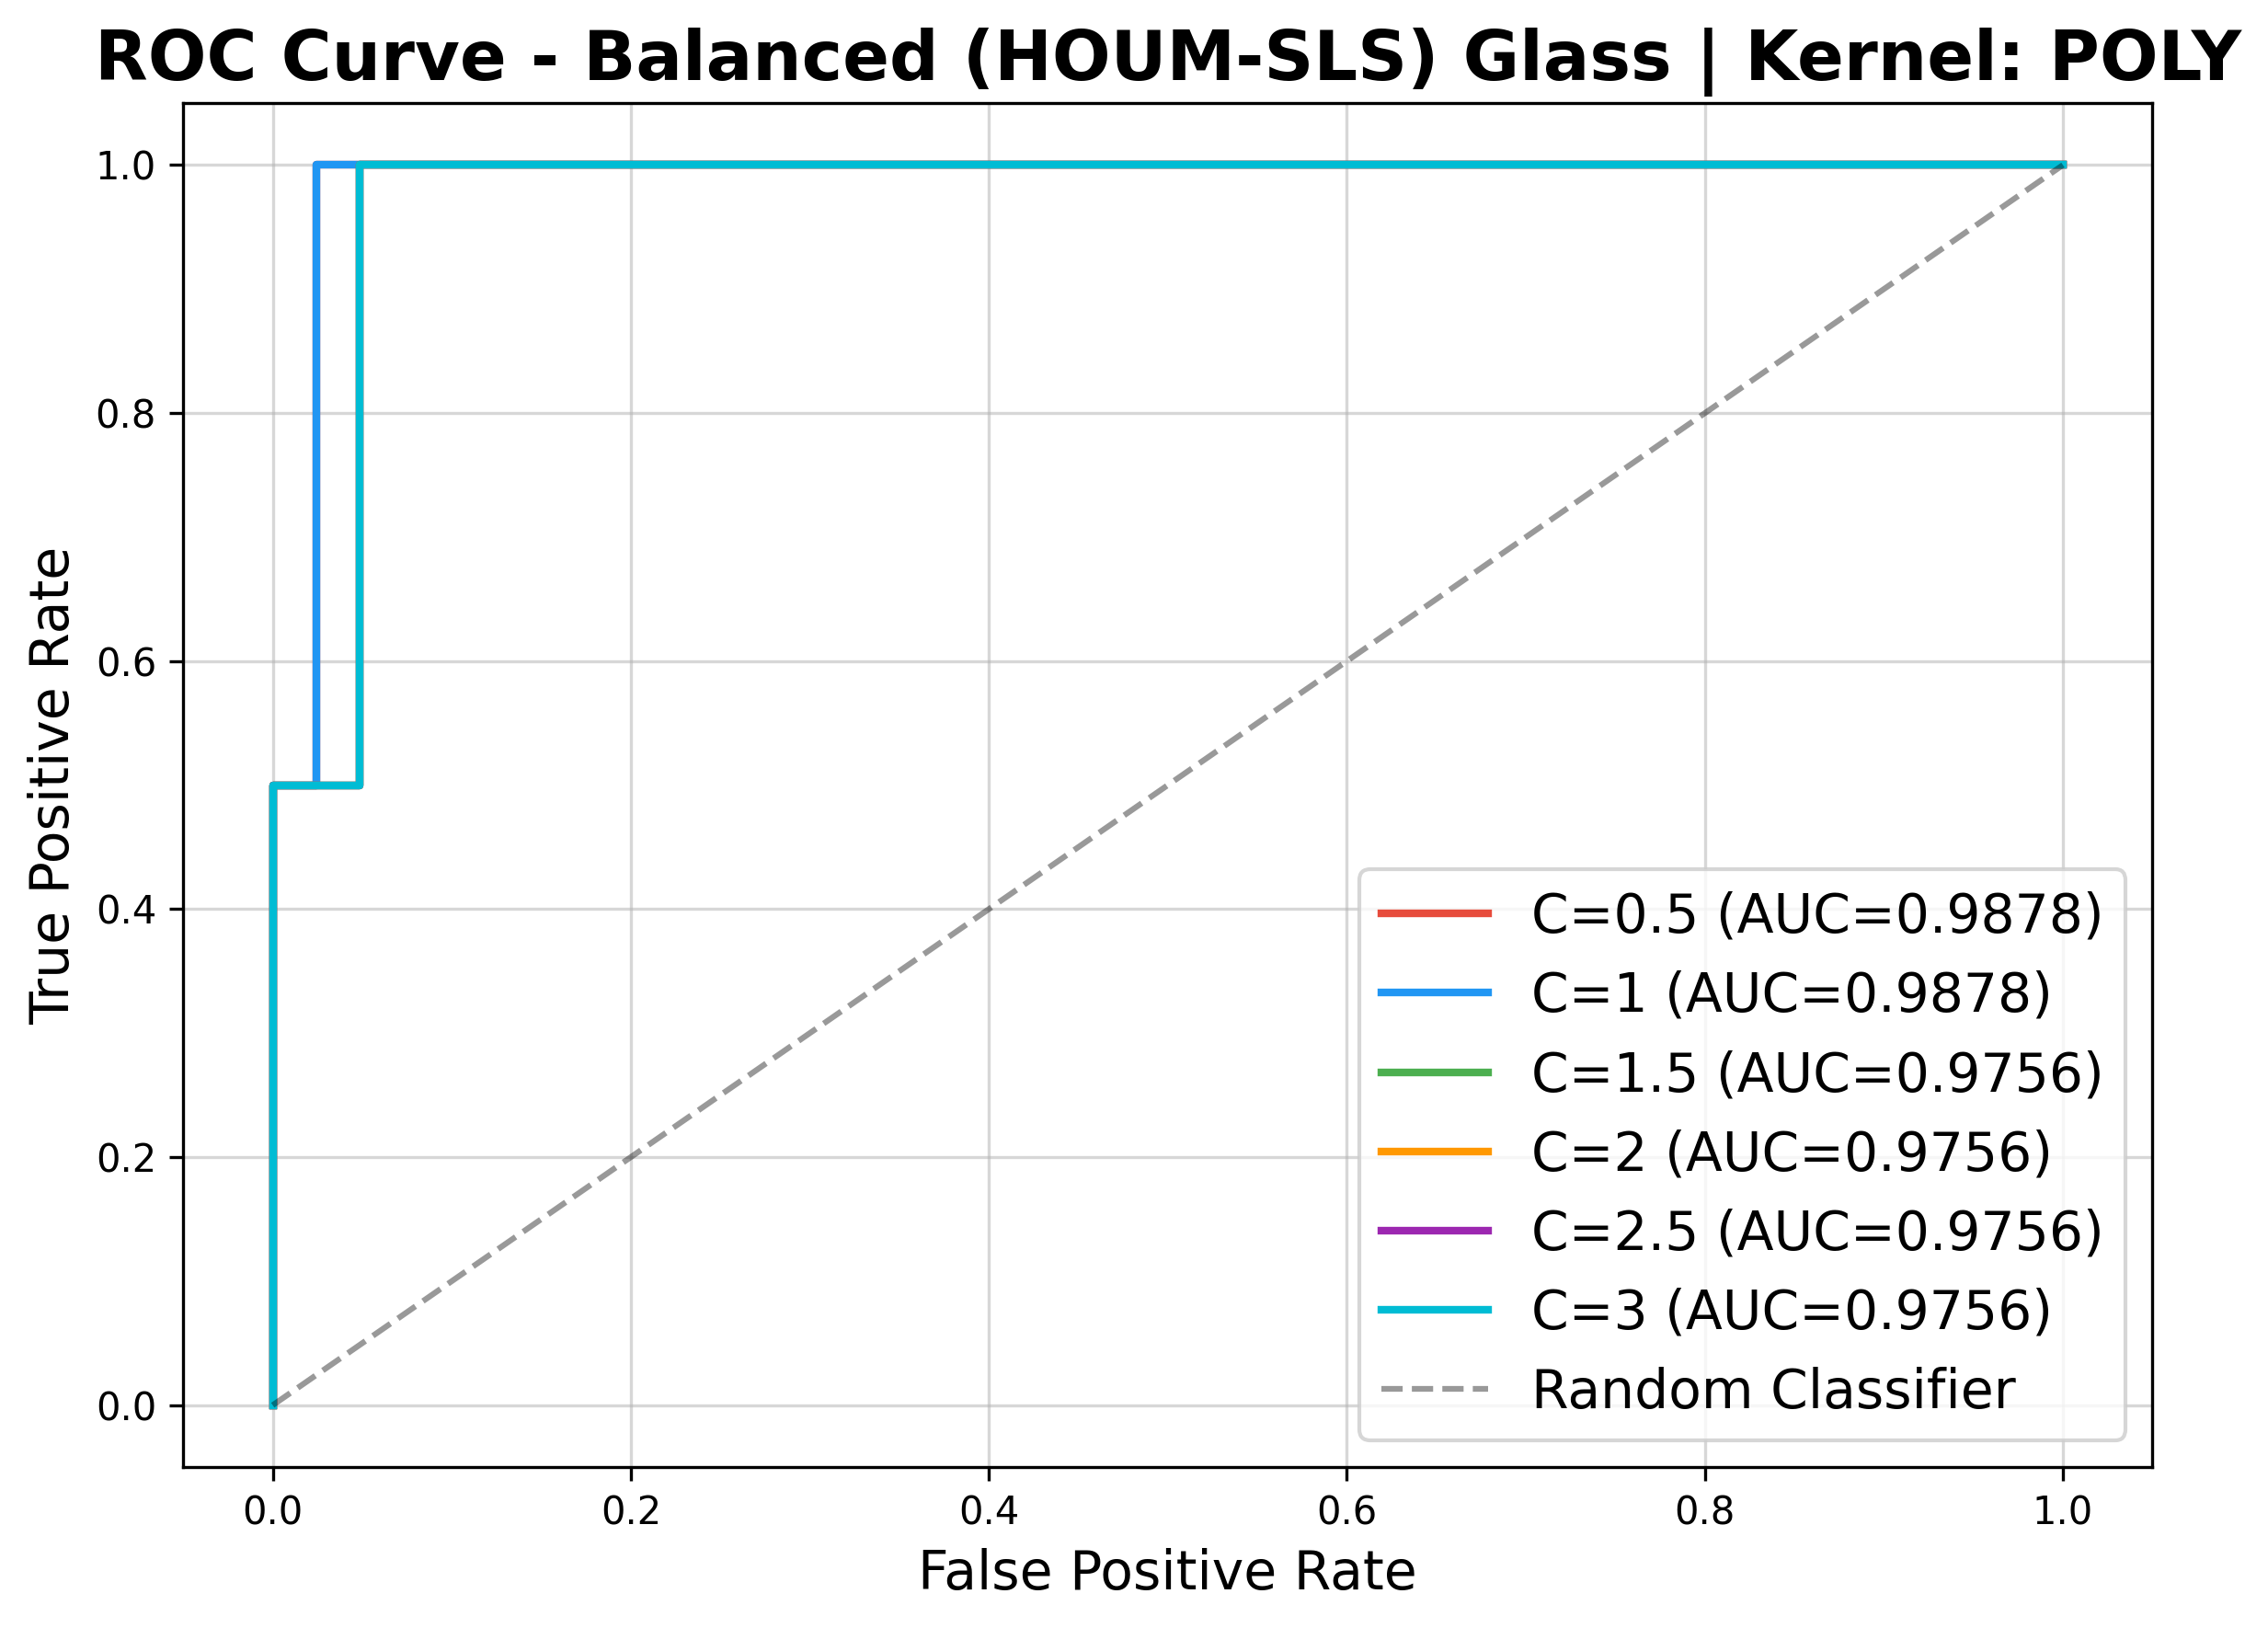
\includegraphics[width=\textwidth]{figure/roc_balanced_glass_sls_kernel_poly.png}
        \caption{Kernel Polynomial}
        \label{fig:4.roc_sls_glass_poly}
    \end{subfigure}
    \caption{Kurva ROC HOUM-SLSMOTE pada Dataset Glass5}
    \label{fig:4.roc_sls_glass}
\end{figure}

Berdasarkan Tabel \ref{table:4.sls_glass}, HOUM-SLSMOTE meningkatkan \textit{Recall} dari 0,5000 (\textit{baseline}) menjadi 1,0000 pada seluruh konfigurasi. Kernel Linear dan Polynomial dengan $C \leq 1$ menghasilkan G-Mean tertinggi sebesar 0,9753 dengan \textit{Precision} 0,5000. Kernel RBF mencatat \textit{Precision} 0,4000 sehingga G-Mean lebih rendah (0,9627). Pada kernel Polynomial $C \geq 1,5$, ROC-AUC menurun menjadi 0,9756. Variasi kernel dan nilai $C$ tidak memengaruhi \textit{Recall} yang tetap 1,0000 di semua konfigurasi, namun memengaruhi \textit{Precision} dan G-Mean.

\subsection{Hasil Metode HOUM dengan ADASYN (HOUM-ADASYN)} \label{IV.HOUM_ADASYN}
Bagian ini menyajikan hasil klasifikasi setelah data diseimbangkan menggunakan metode HOUM dengan ADASYN sebagai komponen \textit{oversampling}. Seluruh kombinasi parameter SVM yang sama dengan HOUM-SLSMOTE diuji pada masing-masing dataset. Hasil metrik evaluasi untuk setiap kombinasi konfigurasi ditampilkan pada tabel berikut, dengan nilai terbaik pada setiap metrik dicetak tebal.

\subsubsection{Dataset Diabetes} \label{IV.ADASYN_Diabetes}
Hasil klasifikasi HOUM-ADASYN pada dataset Diabetes untuk seluruh kombinasi kernel dan nilai $C$ ditunjukkan pada Tabel \ref{table:4.adasyn_diabetes}.

\begin{table}[H]
\centering
\caption{Hasil HOUM-ADASYN pada Dataset Diabetes}
\label{table:4.adasyn_diabetes}
\footnotesize
\begin{tabular}{|l|c|c|c|c|c|c|}
\hline
\textbf{No} & \textbf{Kernel} & \textbf{C} & \textbf{ROC-AUC} & \textbf{\textit{Recall}} & \textbf{\textit{Precision}} & \textbf{G-Mean} \\
\hline
1 & Linear & 0,5 & 0,7767 & 0,6111 & 0,6111 & 0,6948 \\
\hline
2 & Linear & 1 & 0,7689 & 0,6111 & 0,6735 & 0,7165 \\
\hline
3 & Linear & 1,5 & 0,7889 & \textbf{0,6296} & 0,6667 & 0,7229 \\
\hline
4 & Linear & 2 & 0,7889 & \textbf{0,6296} & 0,6667 & 0,7229 \\
\hline
5 & Linear & 2,5 & 0,7683 & 0,5741 & 0,6458 & 0,6903 \\
\hline
6 & Linear & 3 & 0,7807 & 0,6111 & 0,6346 & 0,7036 \\
\hline
7 & RBF & 0,5 & 0,8093 & \textbf{0,6296} & 0,7234 & \textbf{0,7401} \\
\hline
8 & RBF & 1 & 0,8122 & 0,5926 & 0,6667 & 0,7055 \\
\hline
9 & RBF & 1,5 & \textbf{0,8191} & 0,5556 & 0,6122 & 0,6708 \\
\hline
10 & RBF & 2 & 0,8094 & 0,6111 & 0,6346 & 0,7036 \\
\hline
11 & RBF & 2,5 & 0,8033 & 0,6111 & 0,6600 & 0,7122 \\
\hline
12 & RBF & 3 & 0,8102 & 0,5741 & 0,6739 & 0,6985 \\
\hline
13 & Poly & 0,5 & 0,7891 & 0,5556 & 0,6667 & 0,6872 \\
\hline
14 & Poly & 1 & 0,7819 & 0,5556 & 0,6977 & 0,6952 \\
\hline
15 & Poly & 1,5 & 0,8052 & \textbf{0,6296} & 0,6667 & 0,7229 \\
\hline
16 & Poly & 2 & 0,7878 & \textbf{0,6296} & 0,6415 & 0,7141 \\
\hline
17 & Poly & 2,5 & 0,7920 & 0,5926 & \textbf{0,7273} & 0,7221 \\
\hline
18 & Poly & 3 & 0,7898 & 0,5926 & 0,6154 & 0,6885 \\
\hline
\end{tabular}
\end{table}

Kurva ROC untuk masing-masing kernel pada dataset Diabetes ditunjukkan pada Gambar \ref{fig:4.roc_adasyn_diabetes}.

\begin{figure}[H]
    \centering
    \begin{subfigure}[b]{0.47\textwidth}
        \centering
        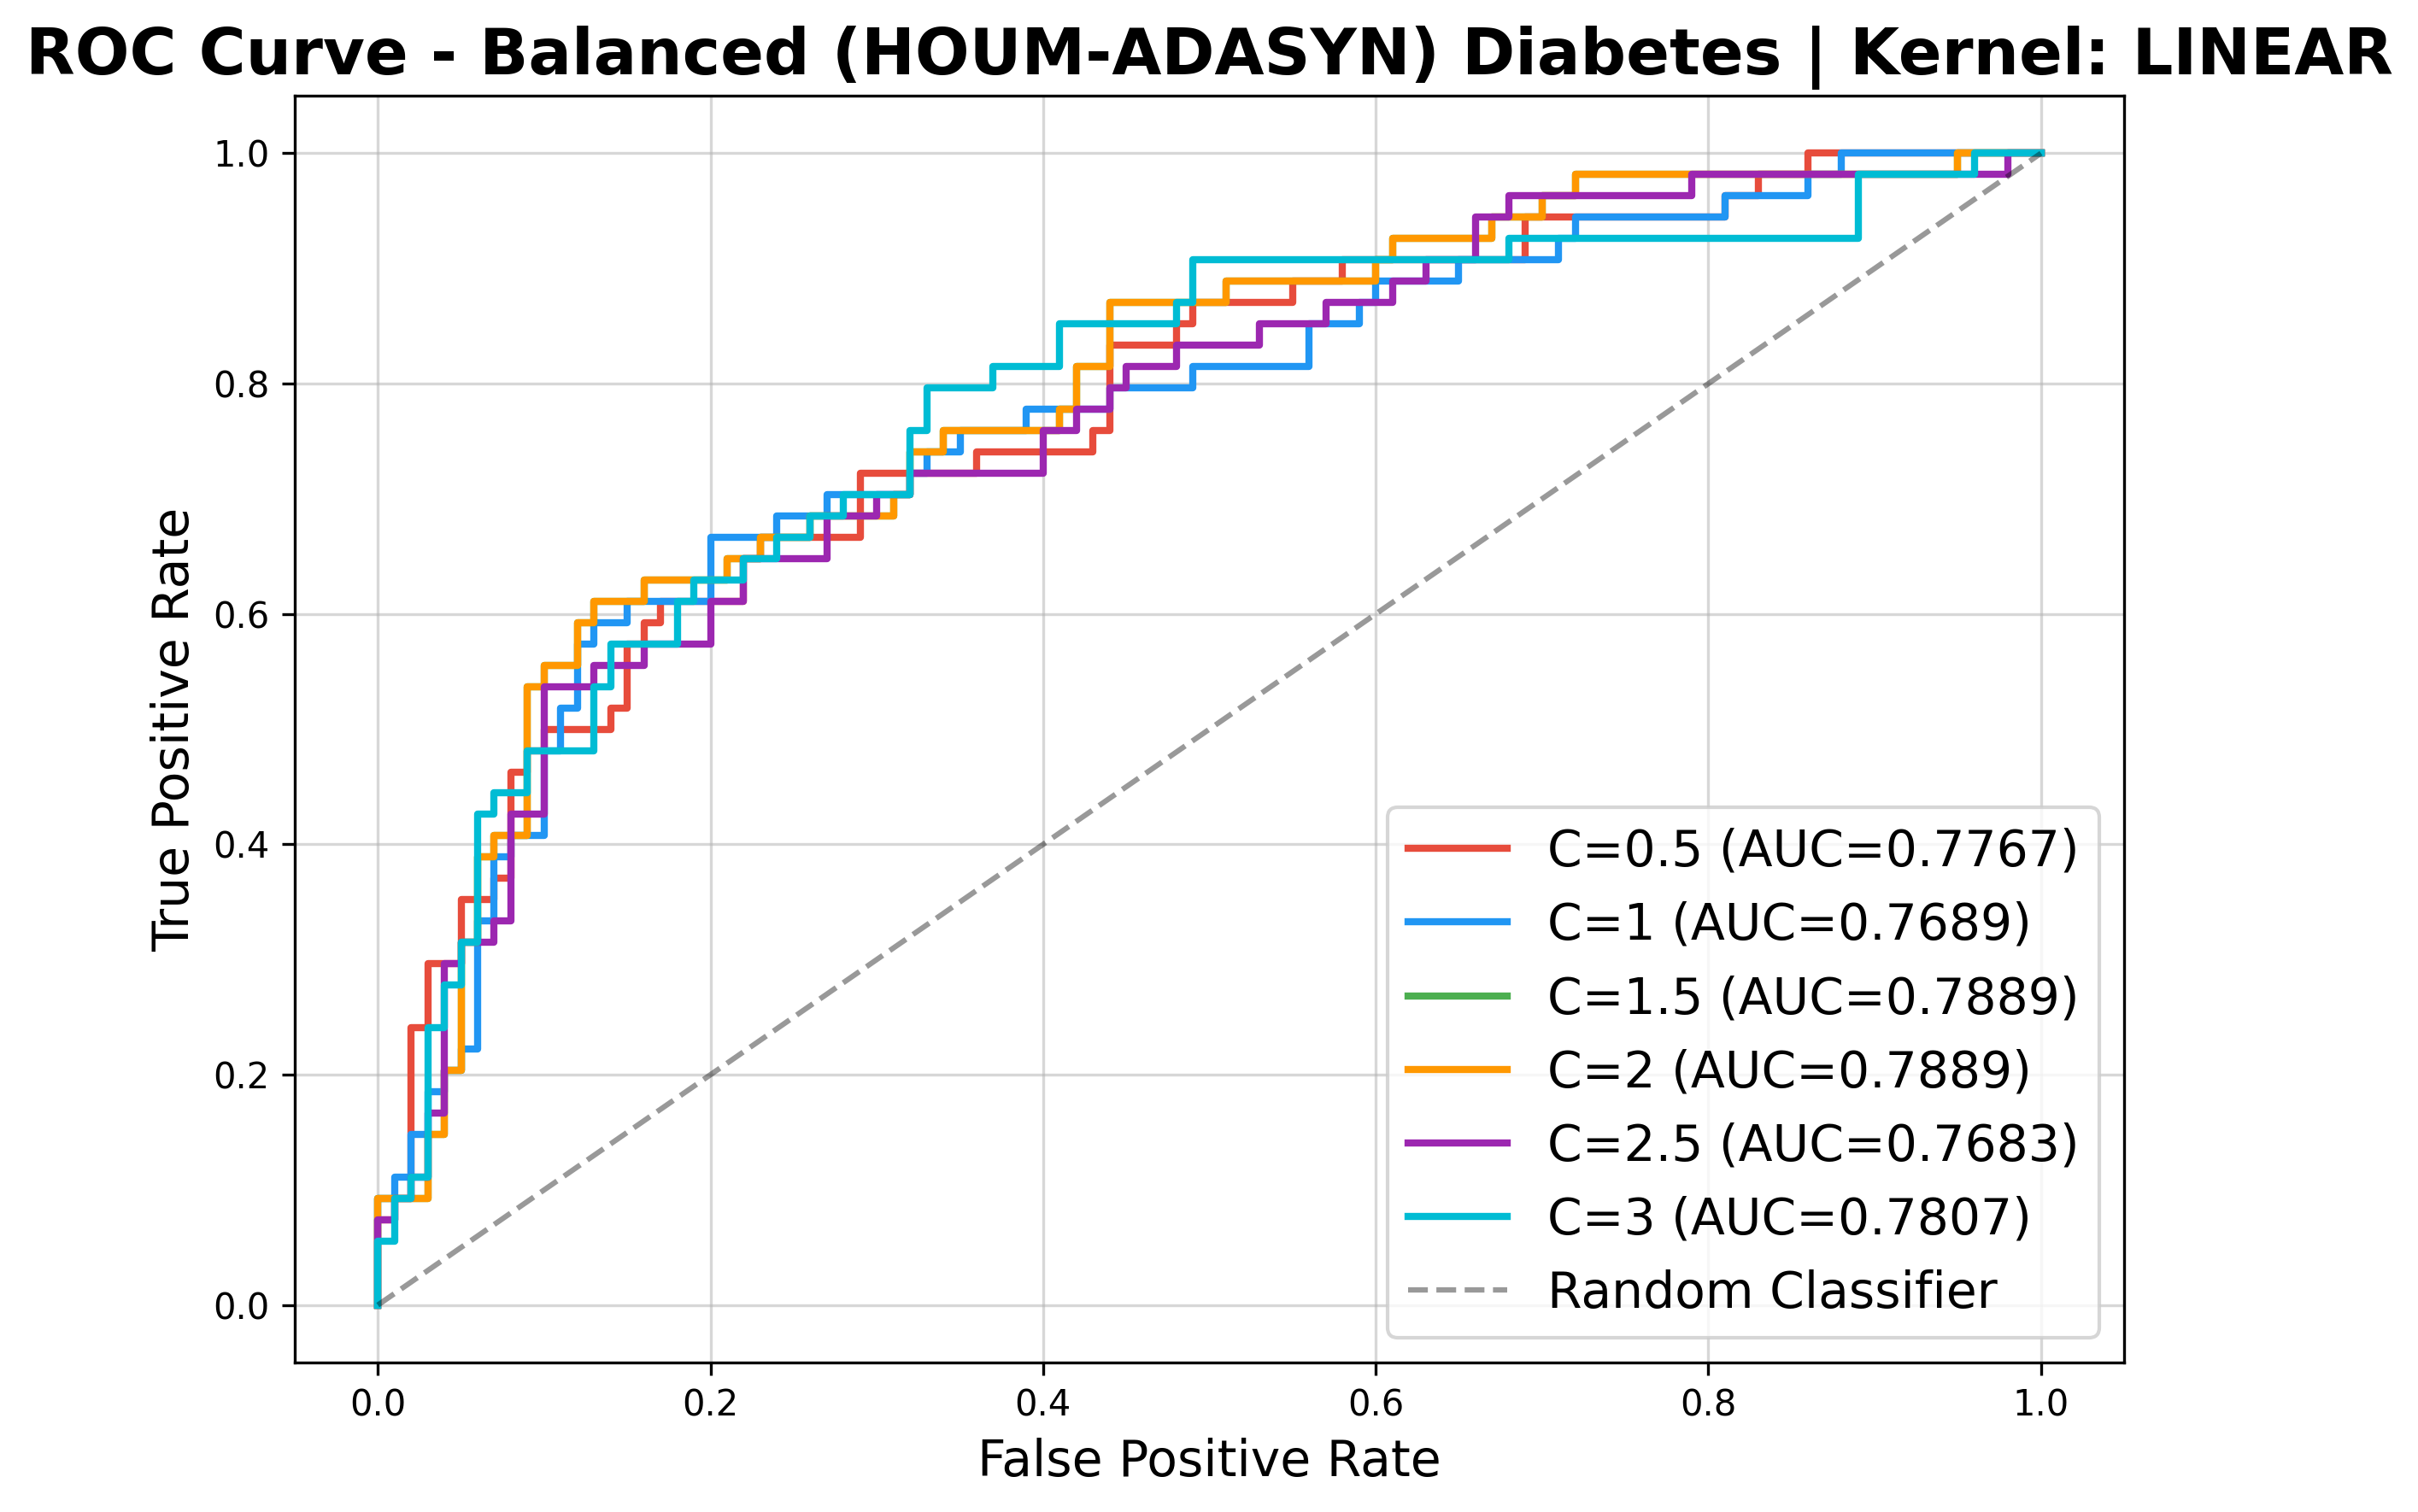
\includegraphics[width=\textwidth]{figure/roc_balanced_diabetes_adasyn_kernel_linear.png}
        \caption{Kernel Linear}
        \label{fig:4.roc_adasyn_diabetes_linear}
    \end{subfigure}
    \hfill
    \begin{subfigure}[b]{0.47\textwidth}
        \centering
        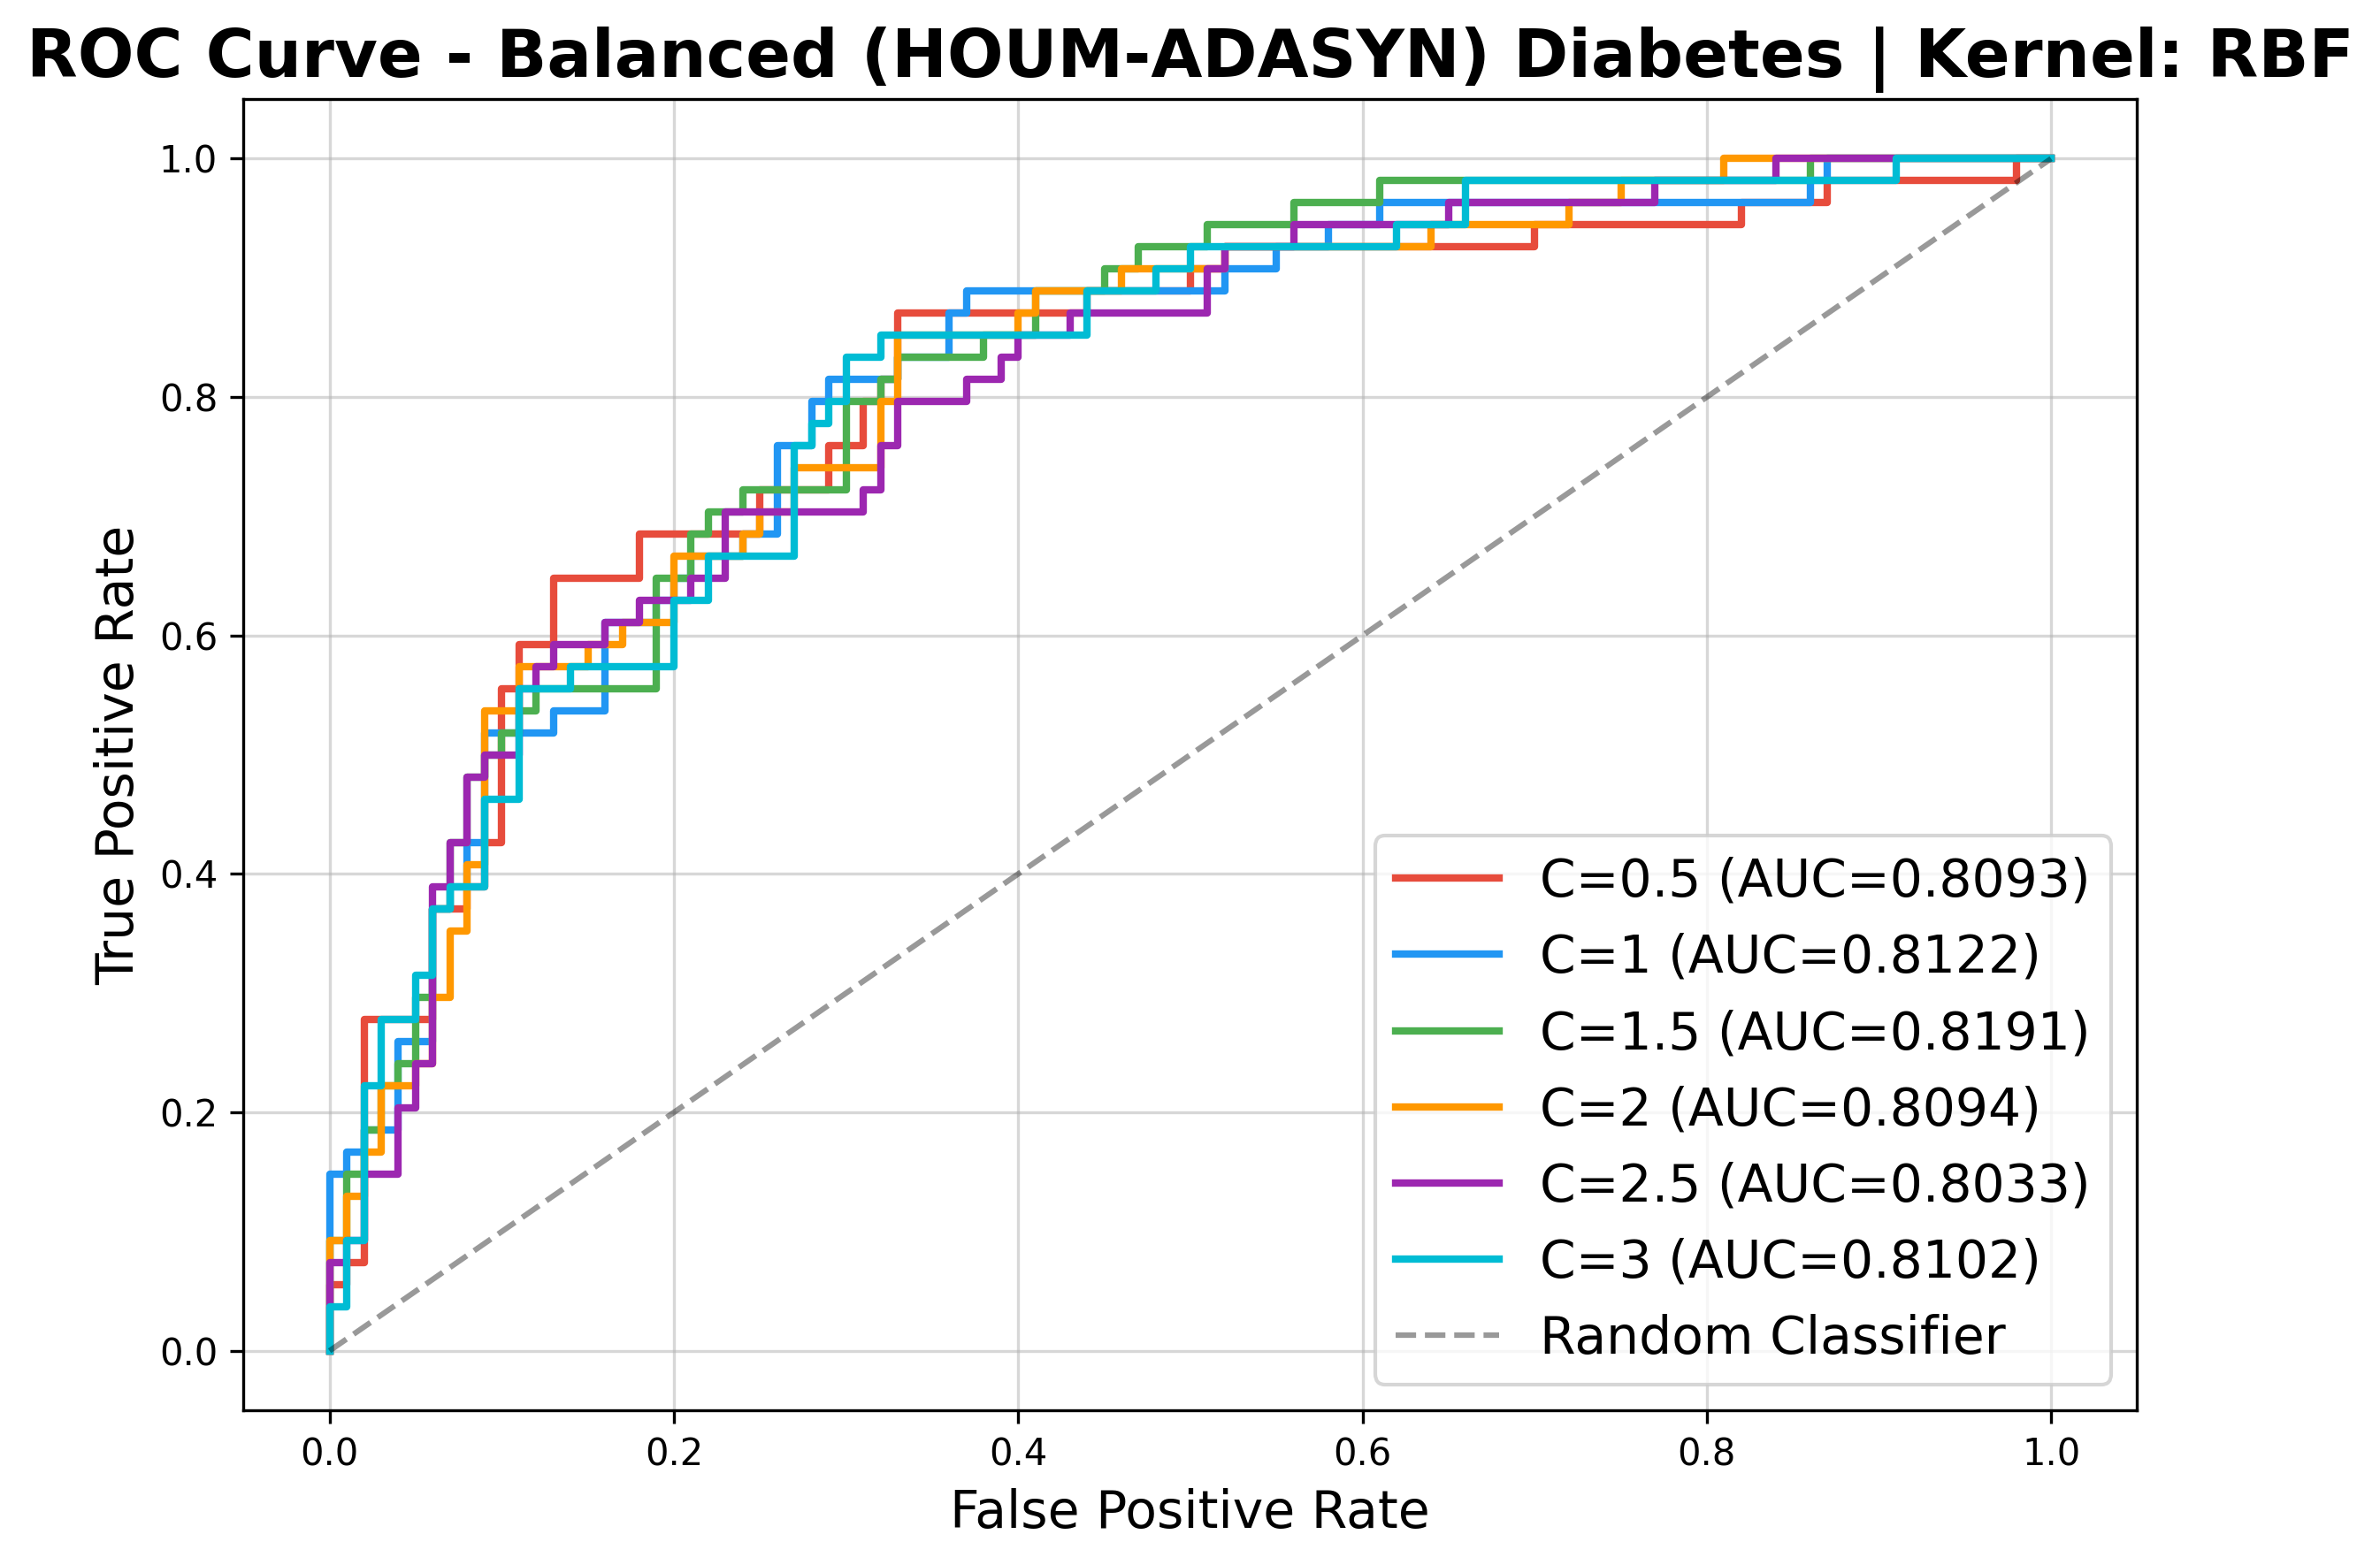
\includegraphics[width=\textwidth]{figure/roc_balanced_diabetes_adasyn_kernel_rbf.png}
        \caption{Kernel RBF}
        \label{fig:4.roc_adasyn_diabetes_rbf}
    \end{subfigure}

    \vspace{0.5em}

    \begin{subfigure}[b]{0.47\textwidth}
        \centering
        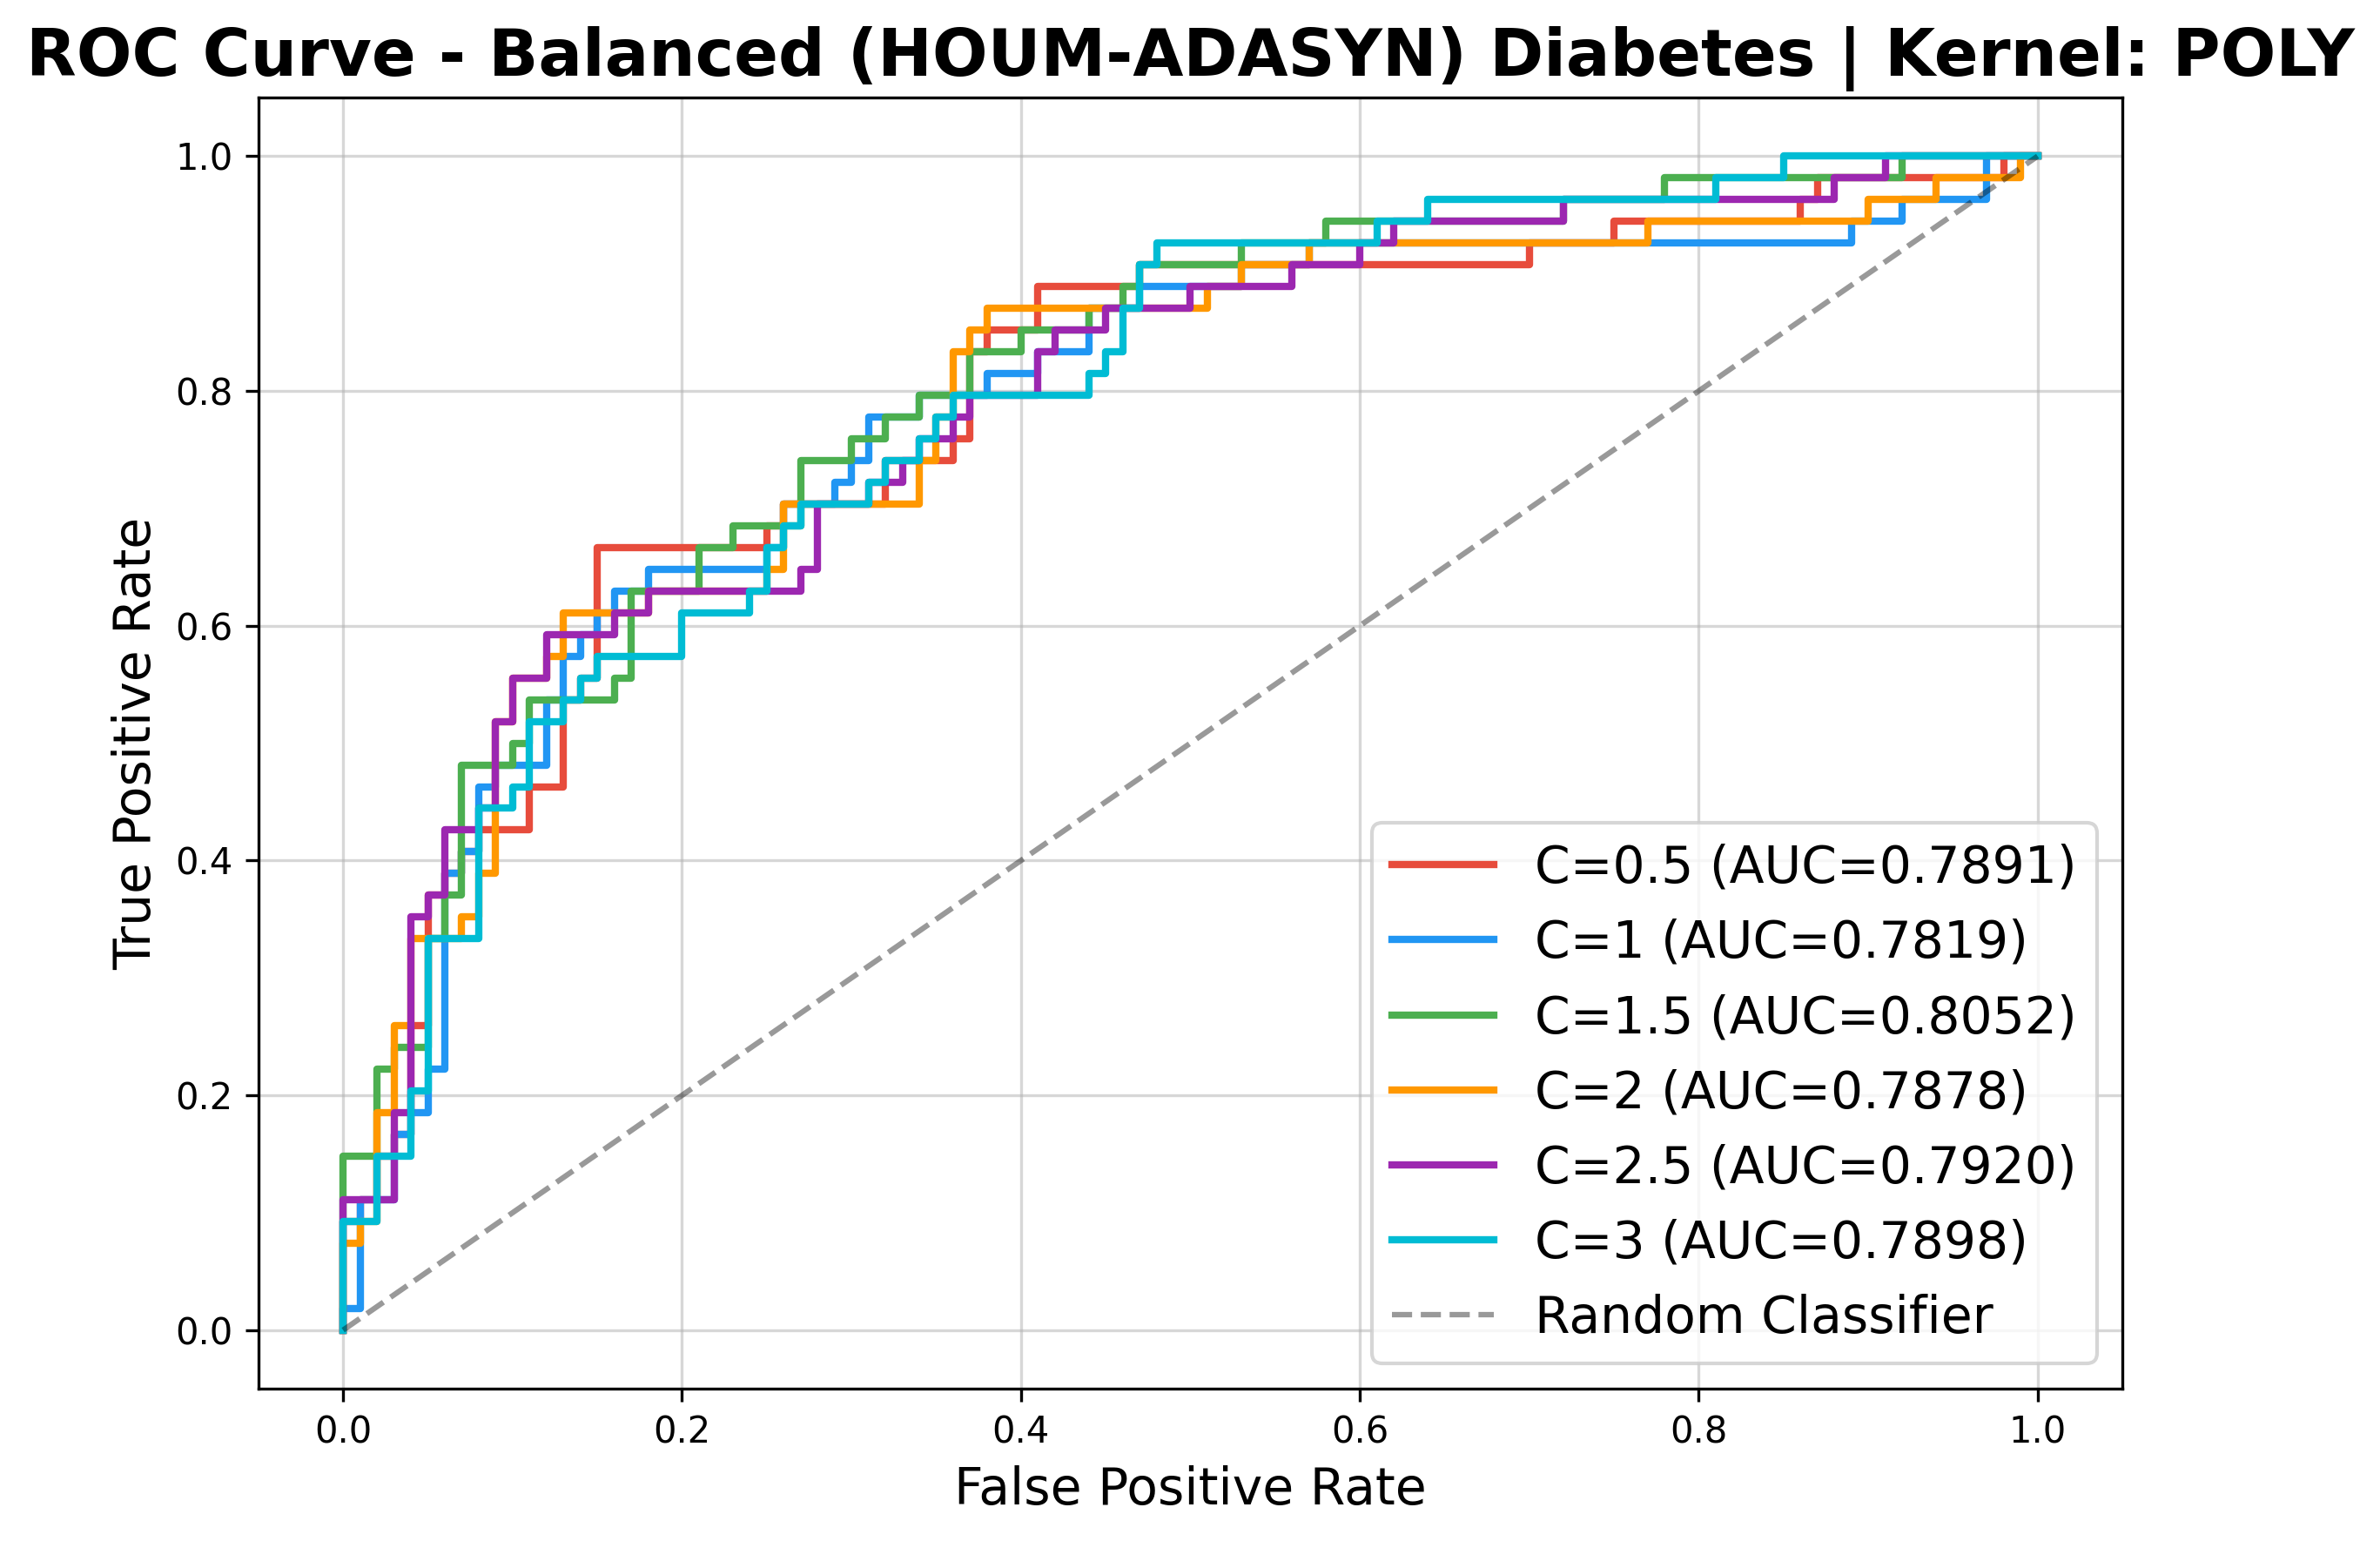
\includegraphics[width=\textwidth]{figure/roc_balanced_diabetes_adasyn_kernel_poly.png}
        \caption{Kernel Polynomial}
        \label{fig:4.roc_adasyn_diabetes_poly}
    \end{subfigure}
    \caption{Kurva ROC HOUM-ADASYN pada Dataset Diabetes}
    \label{fig:4.roc_adasyn_diabetes}
\end{figure}

Berdasarkan Tabel \ref{table:4.adasyn_diabetes}, kernel RBF dengan $C$ = 1,5 menghasilkan ROC-AUC tertinggi sebesar 0,8191, sedangkan G-Mean 0,7401 dan \textit{Precision} 0,7234 dicapai oleh kernel RBF dengan $C$ = 0,5. Nilai \textit{Recall} tertinggi (0,6296) diperoleh oleh beberapa konfigurasi kernel Linear, RBF, dan Polynomial. Dibandingkan HOUM-SLSMOTE, \textit{Recall} HOUM-ADASYN (0,6296) berada di bawah HOUM-SLSMOTE (0,6481), namun \textit{Precision} HOUM-ADASYN unggul (0,7234 berbanding 0,6863), yang menunjukkan jumlah \textit{false positive} yang lebih sedikit. \par

\subsubsection{Dataset Haberman} \label{IV.ADASYN_Haberman}
Hasil klasifikasi HOUM-ADASYN pada dataset Haberman untuk seluruh kombinasi kernel dan nilai $C$ ditunjukkan pada Tabel \ref{table:4.adasyn_haberman}.

\begin{table}[H]
\centering
\caption{Hasil HOUM-ADASYN pada Dataset Haberman}
\label{table:4.adasyn_haberman}
\footnotesize
\begin{tabular}{|l|c|c|c|c|c|c|}
\hline
\textbf{No} & \textbf{Kernel} & \textbf{C} & \textbf{ROC-AUC} & \textbf{\textit{Recall}} & \textbf{\textit{Precision}} & \textbf{G-Mean} \\
\hline
1 & Linear & 0,5 & 0,5462 & 0,2500 & 0,2353 & 0,4235 \\
\hline
2 & Linear & 1 & \textbf{0,5557} & 0,3125 & \textbf{0,2778} & \textbf{0,4735} \\
\hline
3 & Linear & 1,5 & \textbf{0,5557} & 0,3125 & \textbf{0,2778} & \textbf{0,4735} \\
\hline
4 & Linear & 2 & 0,5421 & 0,3125 & 0,2500 & 0,4589 \\
\hline
5 & Linear & 2,5 & 0,5421 & 0,3125 & 0,2500 & 0,4589 \\
\hline
6 & Linear & 3 & 0,5421 & 0,3125 & 0,2500 & 0,4589 \\
\hline
7 & RBF & 0,5 & 0,4817 & 0,1875 & 0,2143 & 0,3777 \\
\hline
8 & RBF & 1 & 0,4966 & 0,1250 & 0,1667 & 0,3128 \\
\hline
9 & RBF & 1,5 & 0,5197 & 0,1250 & 0,1667 & 0,3128 \\
\hline
10 & RBF & 2 & 0,5442 & 0,1250 & 0,1667 & 0,3128 \\
\hline
11 & RBF & 2,5 & 0,5346 & 0,1250 & 0,1667 & 0,3128 \\
\hline
12 & RBF & 3 & 0,5183 & 0,1250 & 0,1667 & 0,3128 \\
\hline
13 & Poly & 0,5 & 0,3967 & \textbf{0,3750} & 0,2000 & 0,4235 \\
\hline
14 & Poly & 1 & 0,4164 & 0,3125 & 0,1852 & 0,4038 \\
\hline
15 & Poly & 1,5 & 0,4164 & 0,3125 & 0,1852 & 0,4038 \\
\hline
16 & Poly & 2 & 0,4164 & 0,3125 & 0,1852 & 0,4038 \\
\hline
17 & Poly & 2,5 & 0,4164 & 0,3125 & 0,1852 & 0,4038 \\
\hline
18 & Poly & 3 & 0,4164 & 0,3125 & 0,1852 & 0,4038 \\
\hline
\end{tabular}
\end{table}

Kurva ROC untuk masing-masing kernel pada dataset Haberman ditunjukkan pada Gambar \ref{fig:4.roc_adasyn_haberman}.

\begin{figure}[H]
    \centering
    \begin{subfigure}[b]{0.47\textwidth}
        \centering
        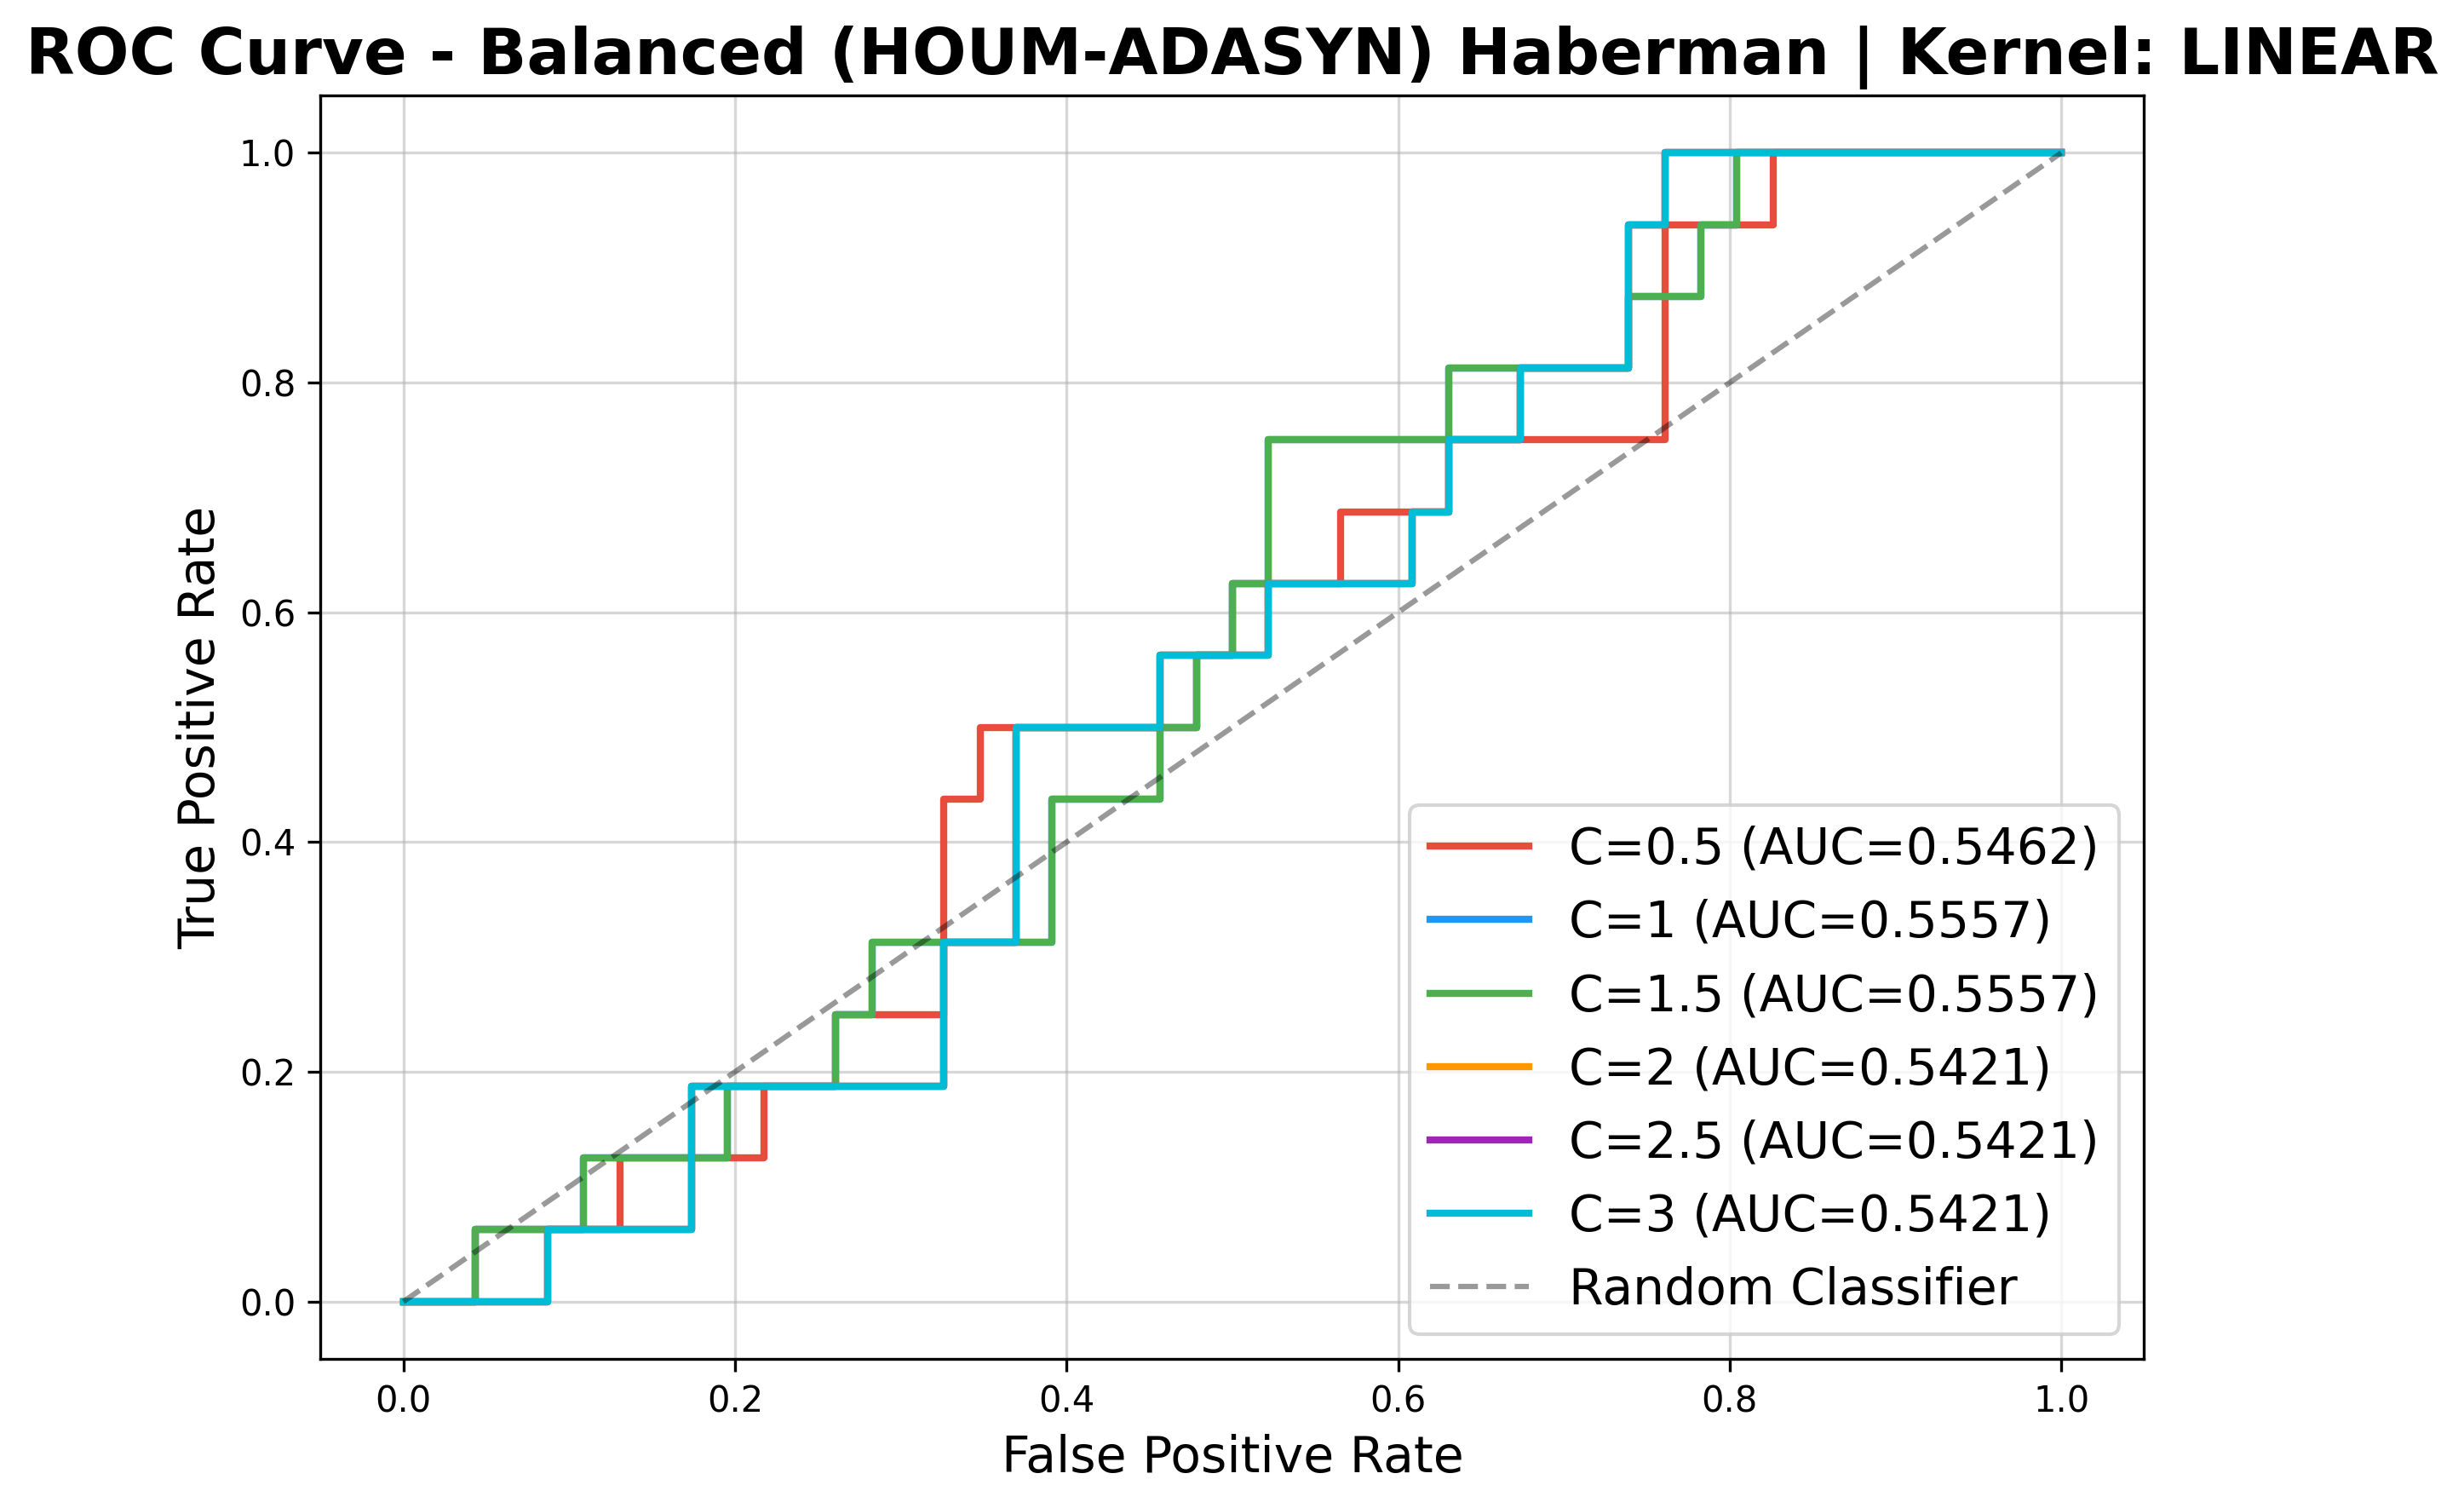
\includegraphics[width=\textwidth]{figure/roc_balanced_haberman_adasyn_kernel_linear.png}
        \caption{Kernel Linear}
        \label{fig:4.roc_adasyn_haberman_linear}
    \end{subfigure}
    \hfill
    \begin{subfigure}[b]{0.47\textwidth}
        \centering
        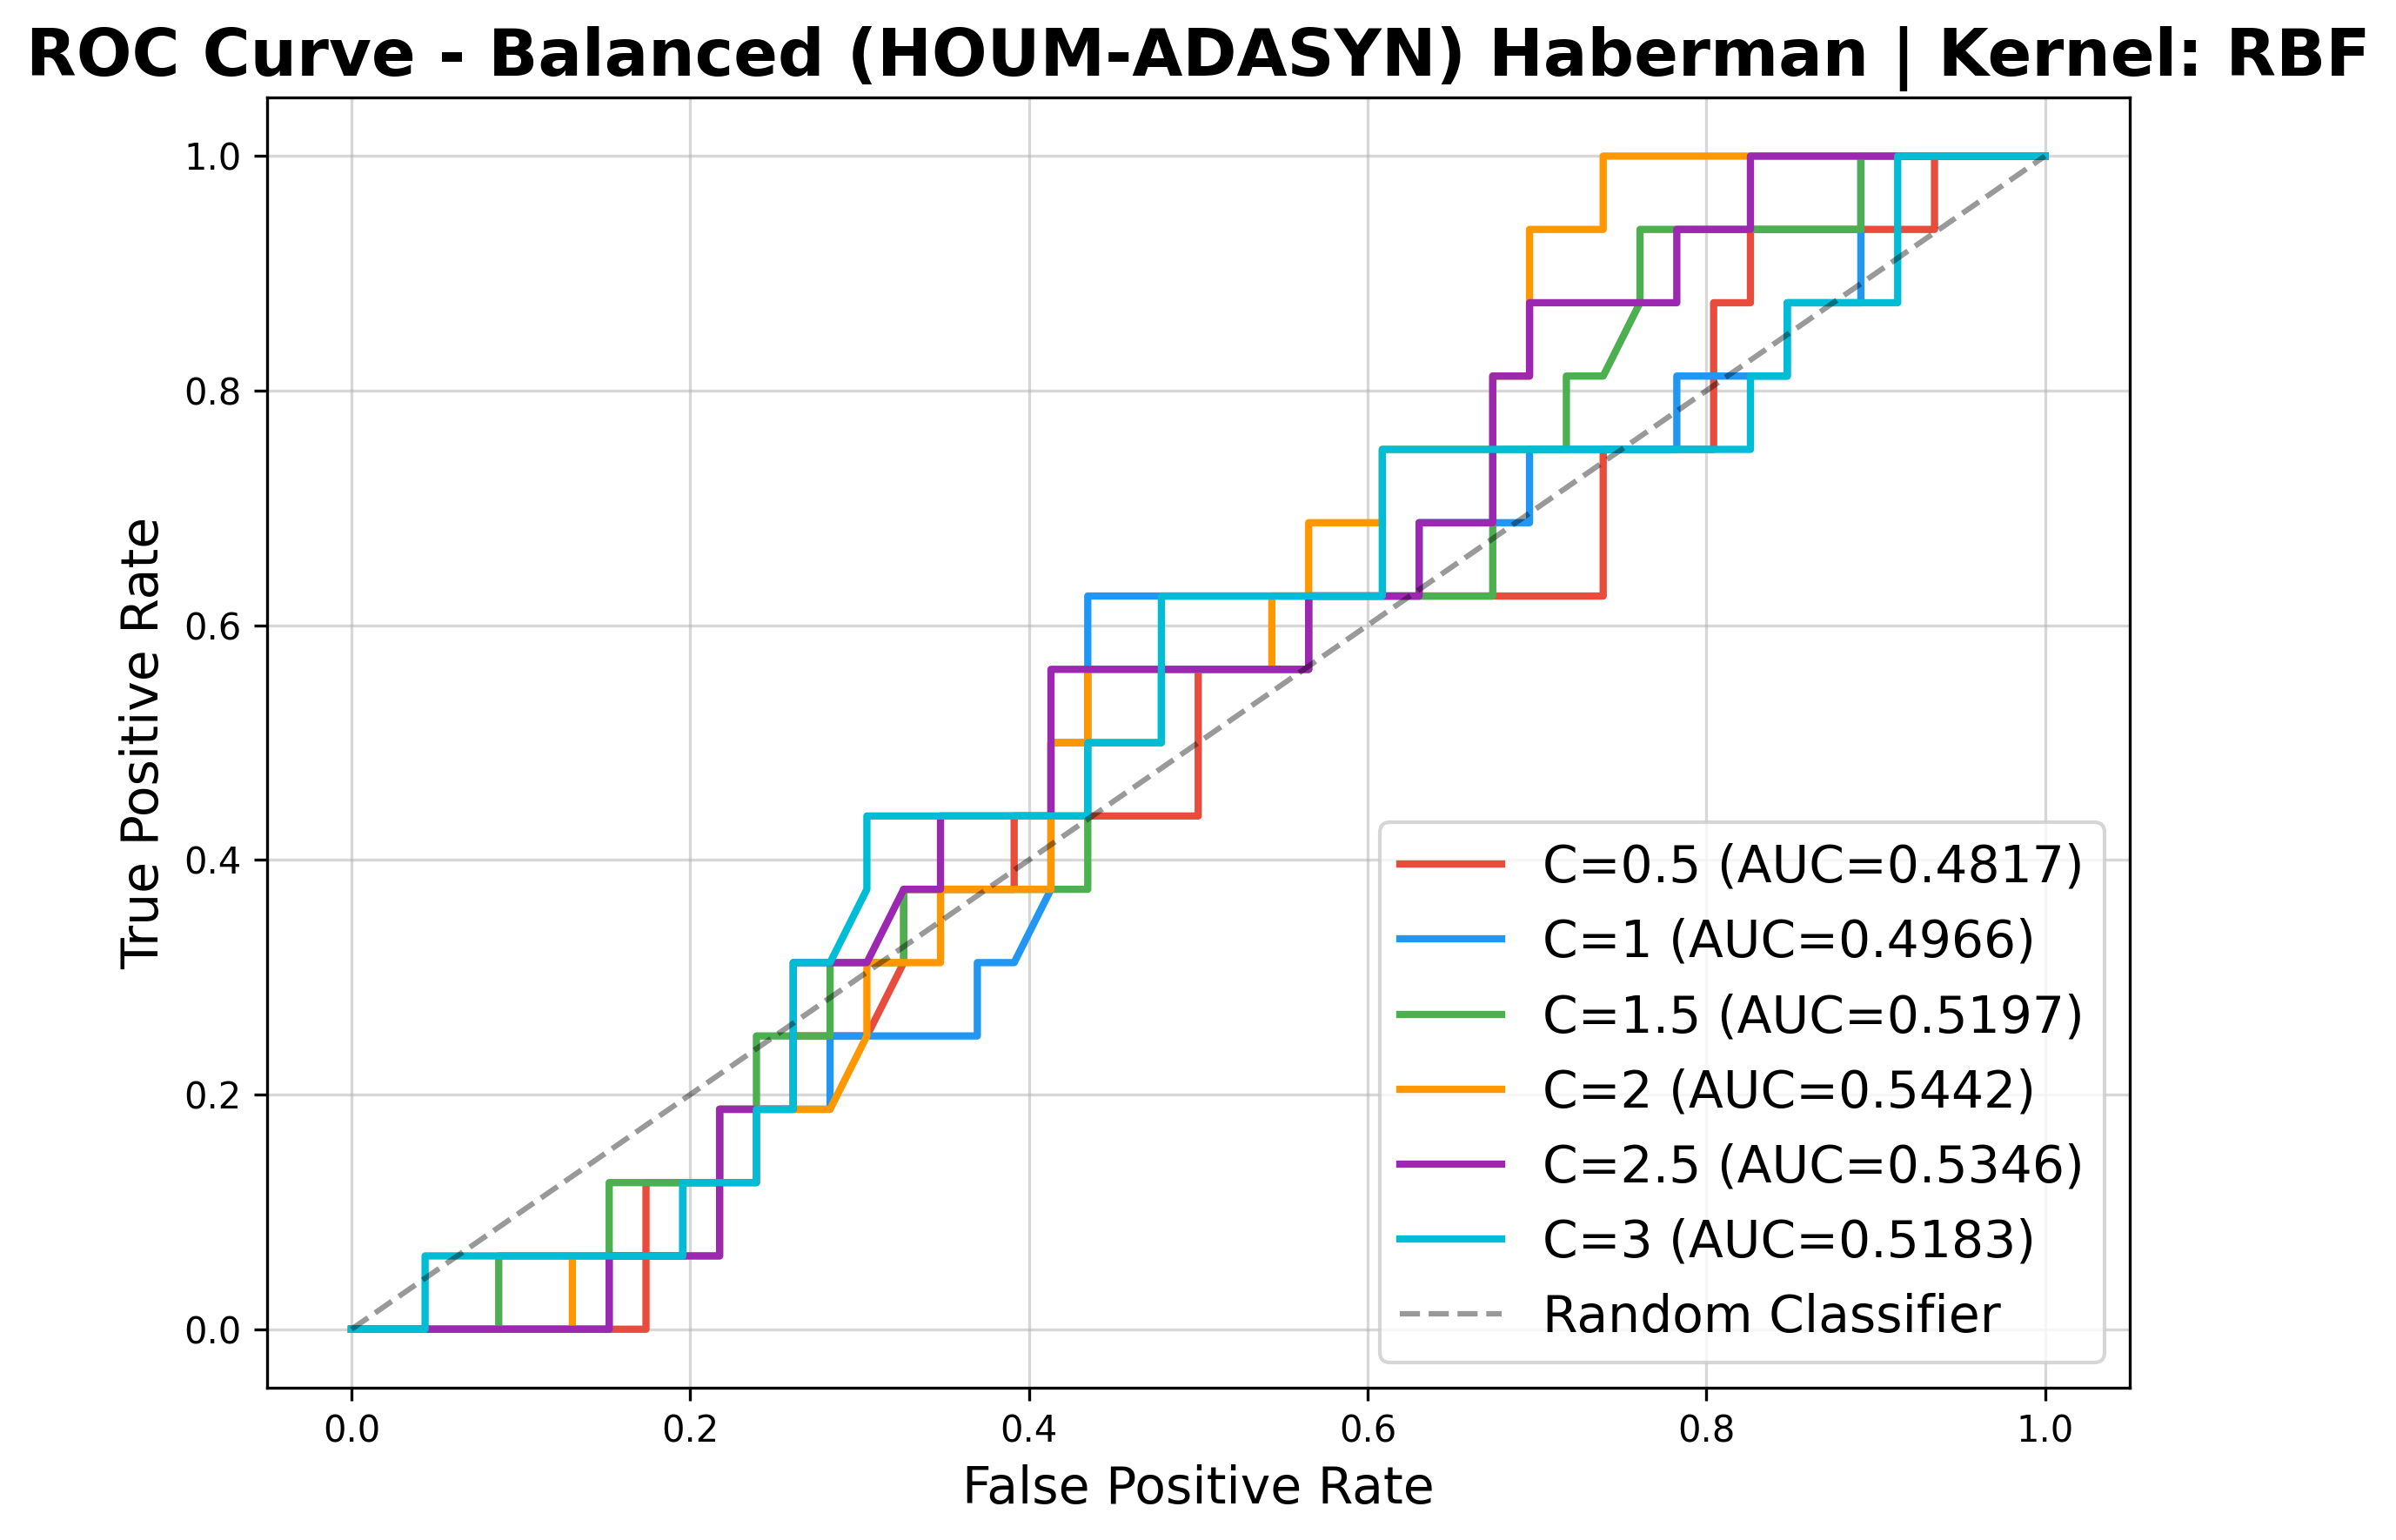
\includegraphics[width=\textwidth]{figure/roc_balanced_haberman_adasyn_kernel_rbf.png}
        \caption{Kernel RBF}
        \label{fig:4.roc_adasyn_haberman_rbf}
    \end{subfigure}

    \vspace{0.5em}

    \begin{subfigure}[b]{0.47\textwidth}
        \centering
        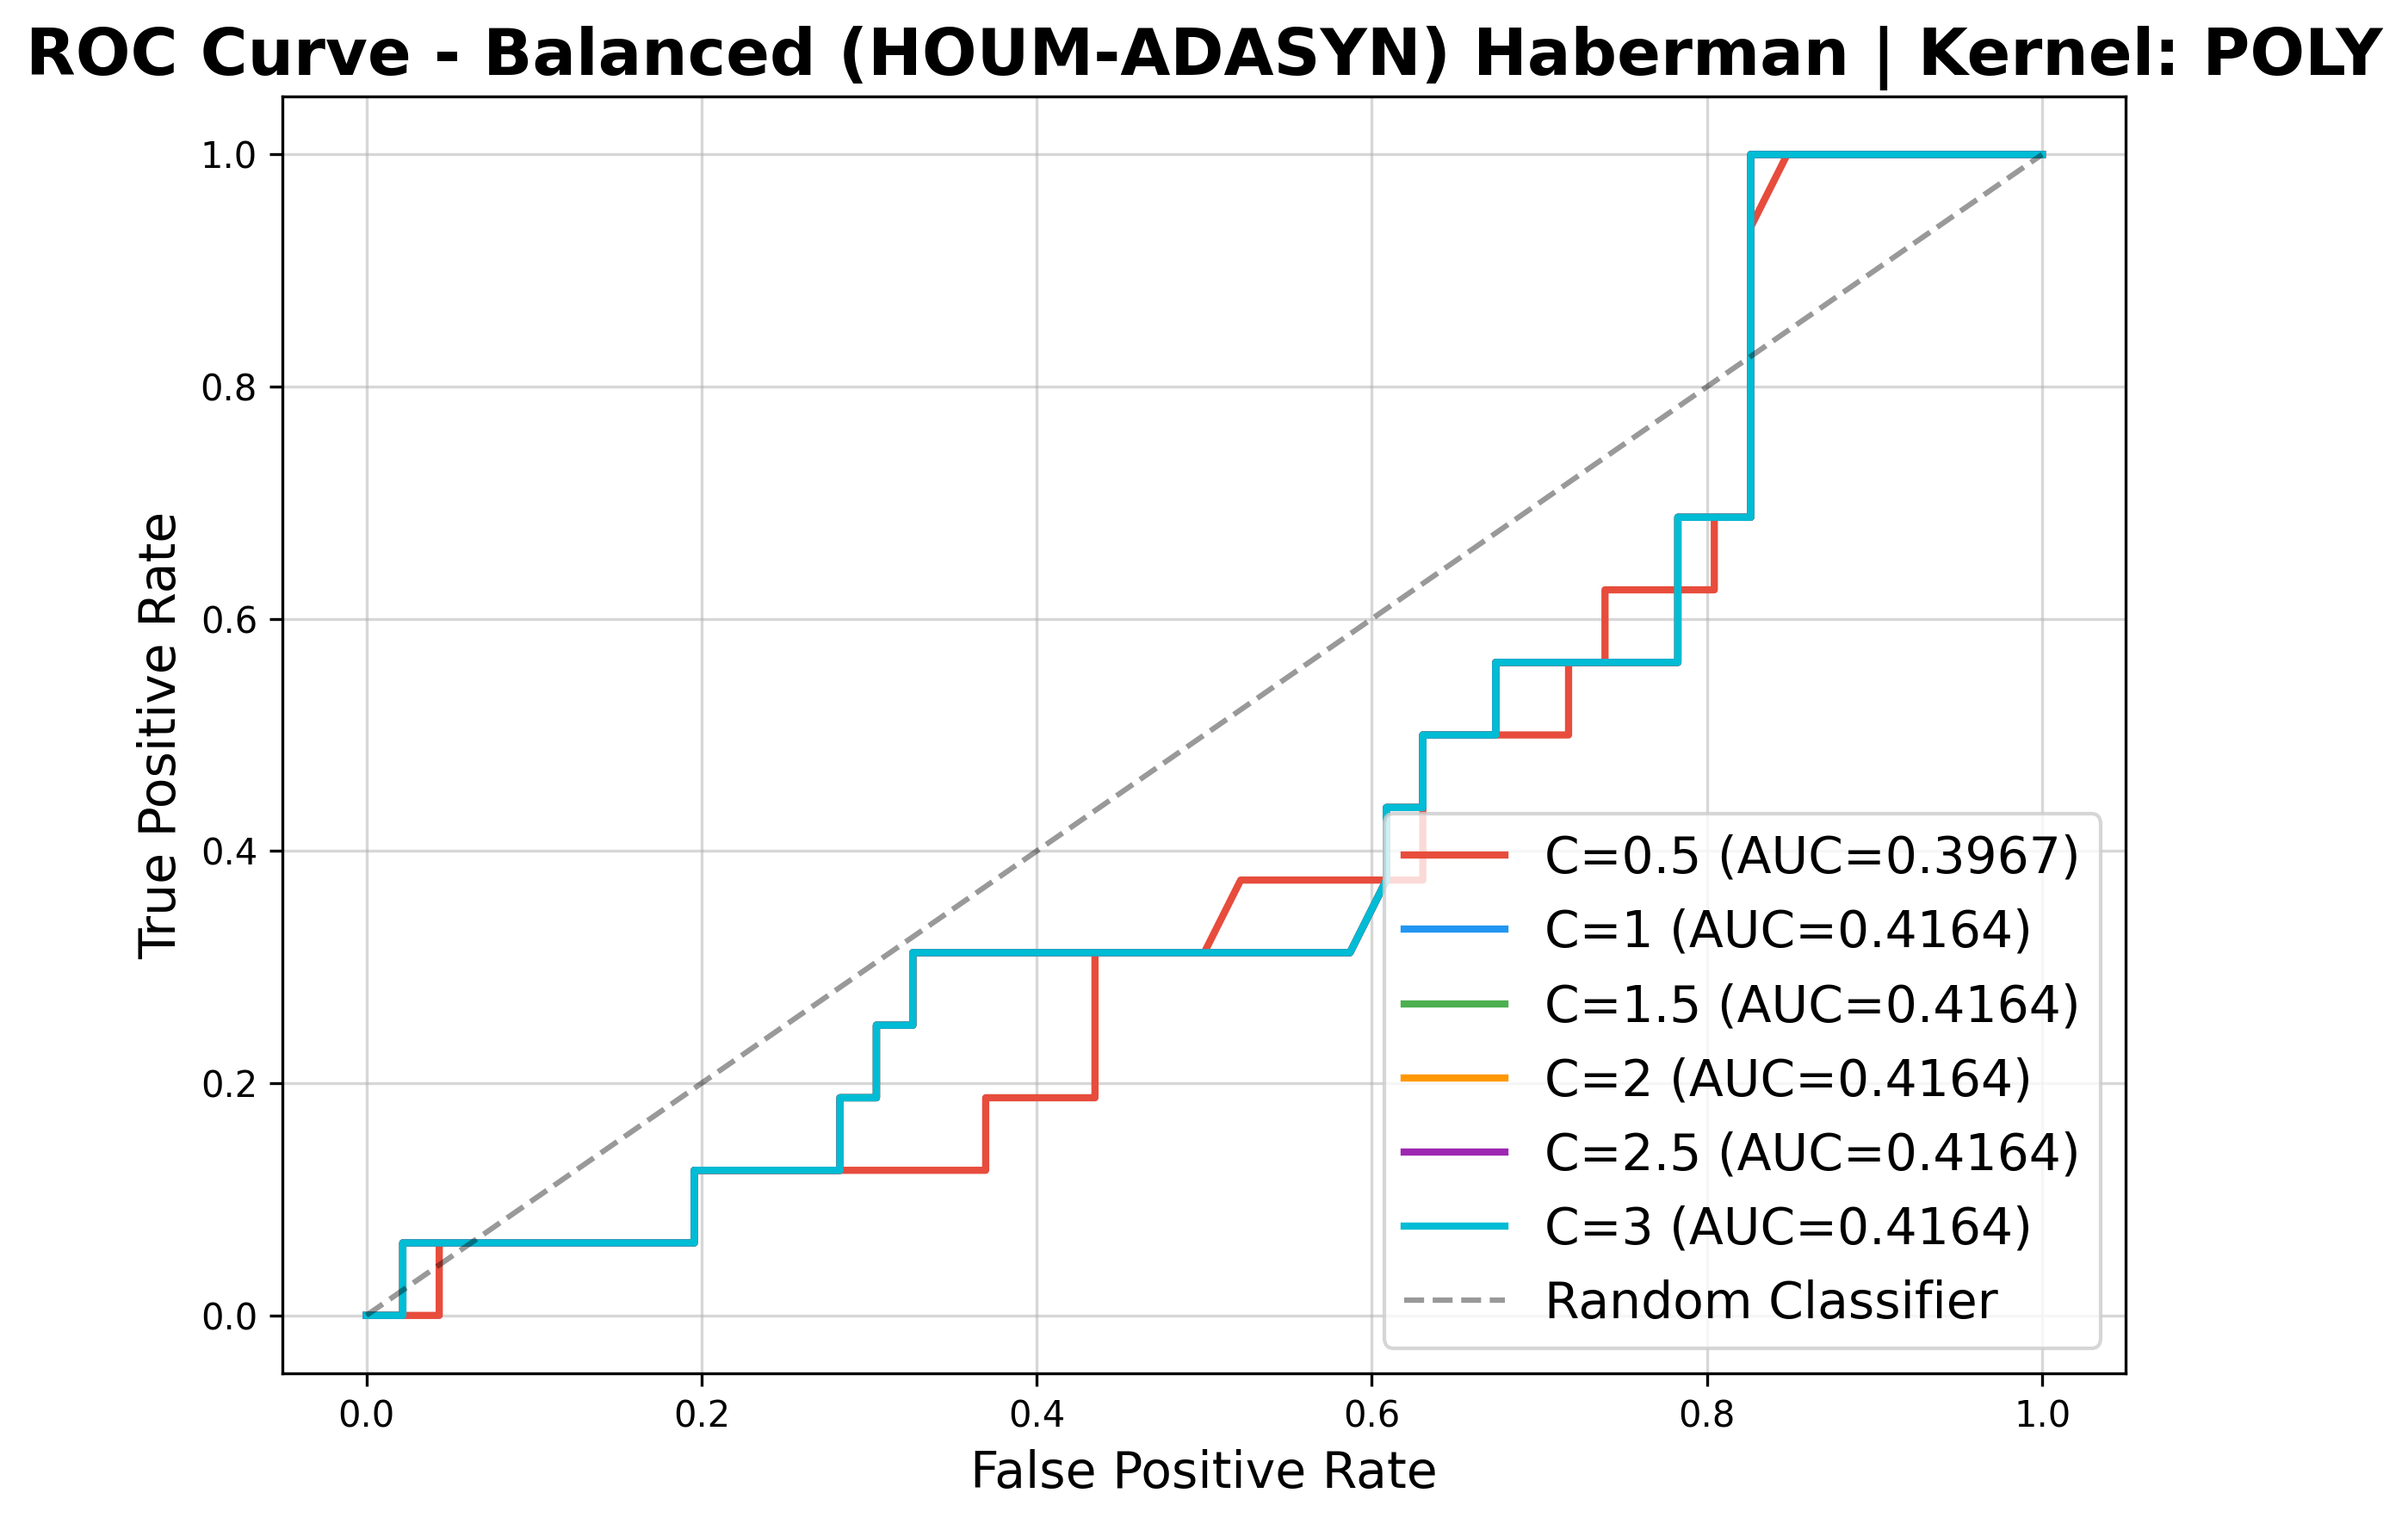
\includegraphics[width=\textwidth]{figure/roc_balanced_haberman_adasyn_kernel_poly.png}
        \caption{Kernel Polynomial}
        \label{fig:4.roc_adasyn_haberman_poly}
    \end{subfigure}
    \caption{Kurva ROC HOUM-ADASYN pada Dataset Haberman}
    \label{fig:4.roc_adasyn_haberman}
\end{figure}

Berdasarkan Tabel \ref{table:4.adasyn_haberman}, performa HOUM-ADASYN pada dataset Haberman secara keseluruhan masih rendah. ROC-AUC tertinggi sebesar 0,5557 dicapai oleh kernel Linear pada $C$ = 1 dan 1,5, dengan G-Mean 0,4735 dan \textit{Precision} 0,2778 pada konfigurasi yang sama. Kernel RBF mencatat \textit{Recall} terendah sebesar 0,1250, mengindikasikan bahwa SVM dengan kernel RBF terlalu agresif menghapus sampel mayoritas. Dibandingkan HOUM-SLSMOTE, \textit{Precision} HOUM-ADASYN sedikit unggul (0,2778 berbanding 0,2500) meskipun metrik lainnya relatif setara. \par

\subsubsection{Dataset Transfusion} \label{IV.ADASYN_Transfusion}
Hasil klasifikasi HOUM-ADASYN pada dataset Transfusion untuk seluruh kombinasi kernel dan nilai $C$ ditunjukkan pada Tabel \ref{table:4.adasyn_transfusion}.

\begin{table}[H]
\centering
\caption{Hasil HOUM-ADASYN pada Dataset Transfusion}
\label{table:4.adasyn_transfusion}
\footnotesize
\begin{tabular}{|l|c|c|c|c|c|c|}
\hline
\textbf{No} & \textbf{Kernel} & \textbf{C} & \textbf{ROC-AUC} & \textbf{\textit{Recall}} & \textbf{\textit{Precision}} & \textbf{G-Mean} \\
\hline
1 & Linear & 0,5 & 0,6868 & 0,6667 & 0,3636 & 0,6489 \\
\hline
2 & Linear & 1 & 0,6913 & 0,6944 & 0,3472 & 0,6389 \\
\hline
3 & Linear & 1,5 & 0,6809 & 0,6944 & 0,3571 & 0,6483 \\
\hline
4 & Linear & 2 & \textbf{0,7004} & 0,6667 & 0,3529 & 0,6398 \\
\hline
5 & Linear & 2,5 & 0,6657 & \textbf{0,7222} & 0,3377 & 0,6318 \\
\hline
6 & Linear & 3 & 0,6430 & 0,4722 & 0,2787 & 0,5385 \\
\hline
7 & RBF & 0,5 & 0,6741 & 0,5833 & 0,3500 & 0,6195 \\
\hline
8 & RBF & 1 & 0,6887 & 0,6667 & \textbf{0,3810} & \textbf{0,6623} \\
\hline
9 & RBF & 1,5 & 0,6740 & 0,6389 & 0,3770 & 0,6526 \\
\hline
10 & RBF & 2 & 0,6814 & 0,5556 & 0,3279 & 0,5964 \\
\hline
11 & RBF & 2,5 & 0,6938 & 0,5556 & 0,3448 & 0,6086 \\
\hline
12 & RBF & 3 & 0,6930 & 0,6111 & 0,3492 & 0,6256 \\
\hline
13 & Poly & 0,5 & 0,6611 & 0,5000 & 0,3214 & 0,5774 \\
\hline
14 & Poly & 1 & 0,6774 & 0,5833 & 0,3559 & 0,6236 \\
\hline
15 & Poly & 1,5 & 0,6854 & 0,5556 & 0,3279 & 0,5964 \\
\hline
16 & Poly & 2 & 0,6788 & 0,5278 & 0,3115 & 0,5774 \\
\hline
17 & Poly & 2,5 & 0,6879 & 0,5556 & 0,3226 & 0,5923 \\
\hline
18 & Poly & 3 & 0,6615 & 0,5000 & 0,2951 & 0,5580 \\
\hline
\end{tabular}
\end{table}

Kurva ROC untuk masing-masing kernel pada dataset Transfusion ditunjukkan pada Gambar \ref{fig:4.roc_adasyn_transfusion}.

\begin{figure}[H]
    \centering
    \begin{subfigure}[b]{0.47\textwidth}
        \centering
        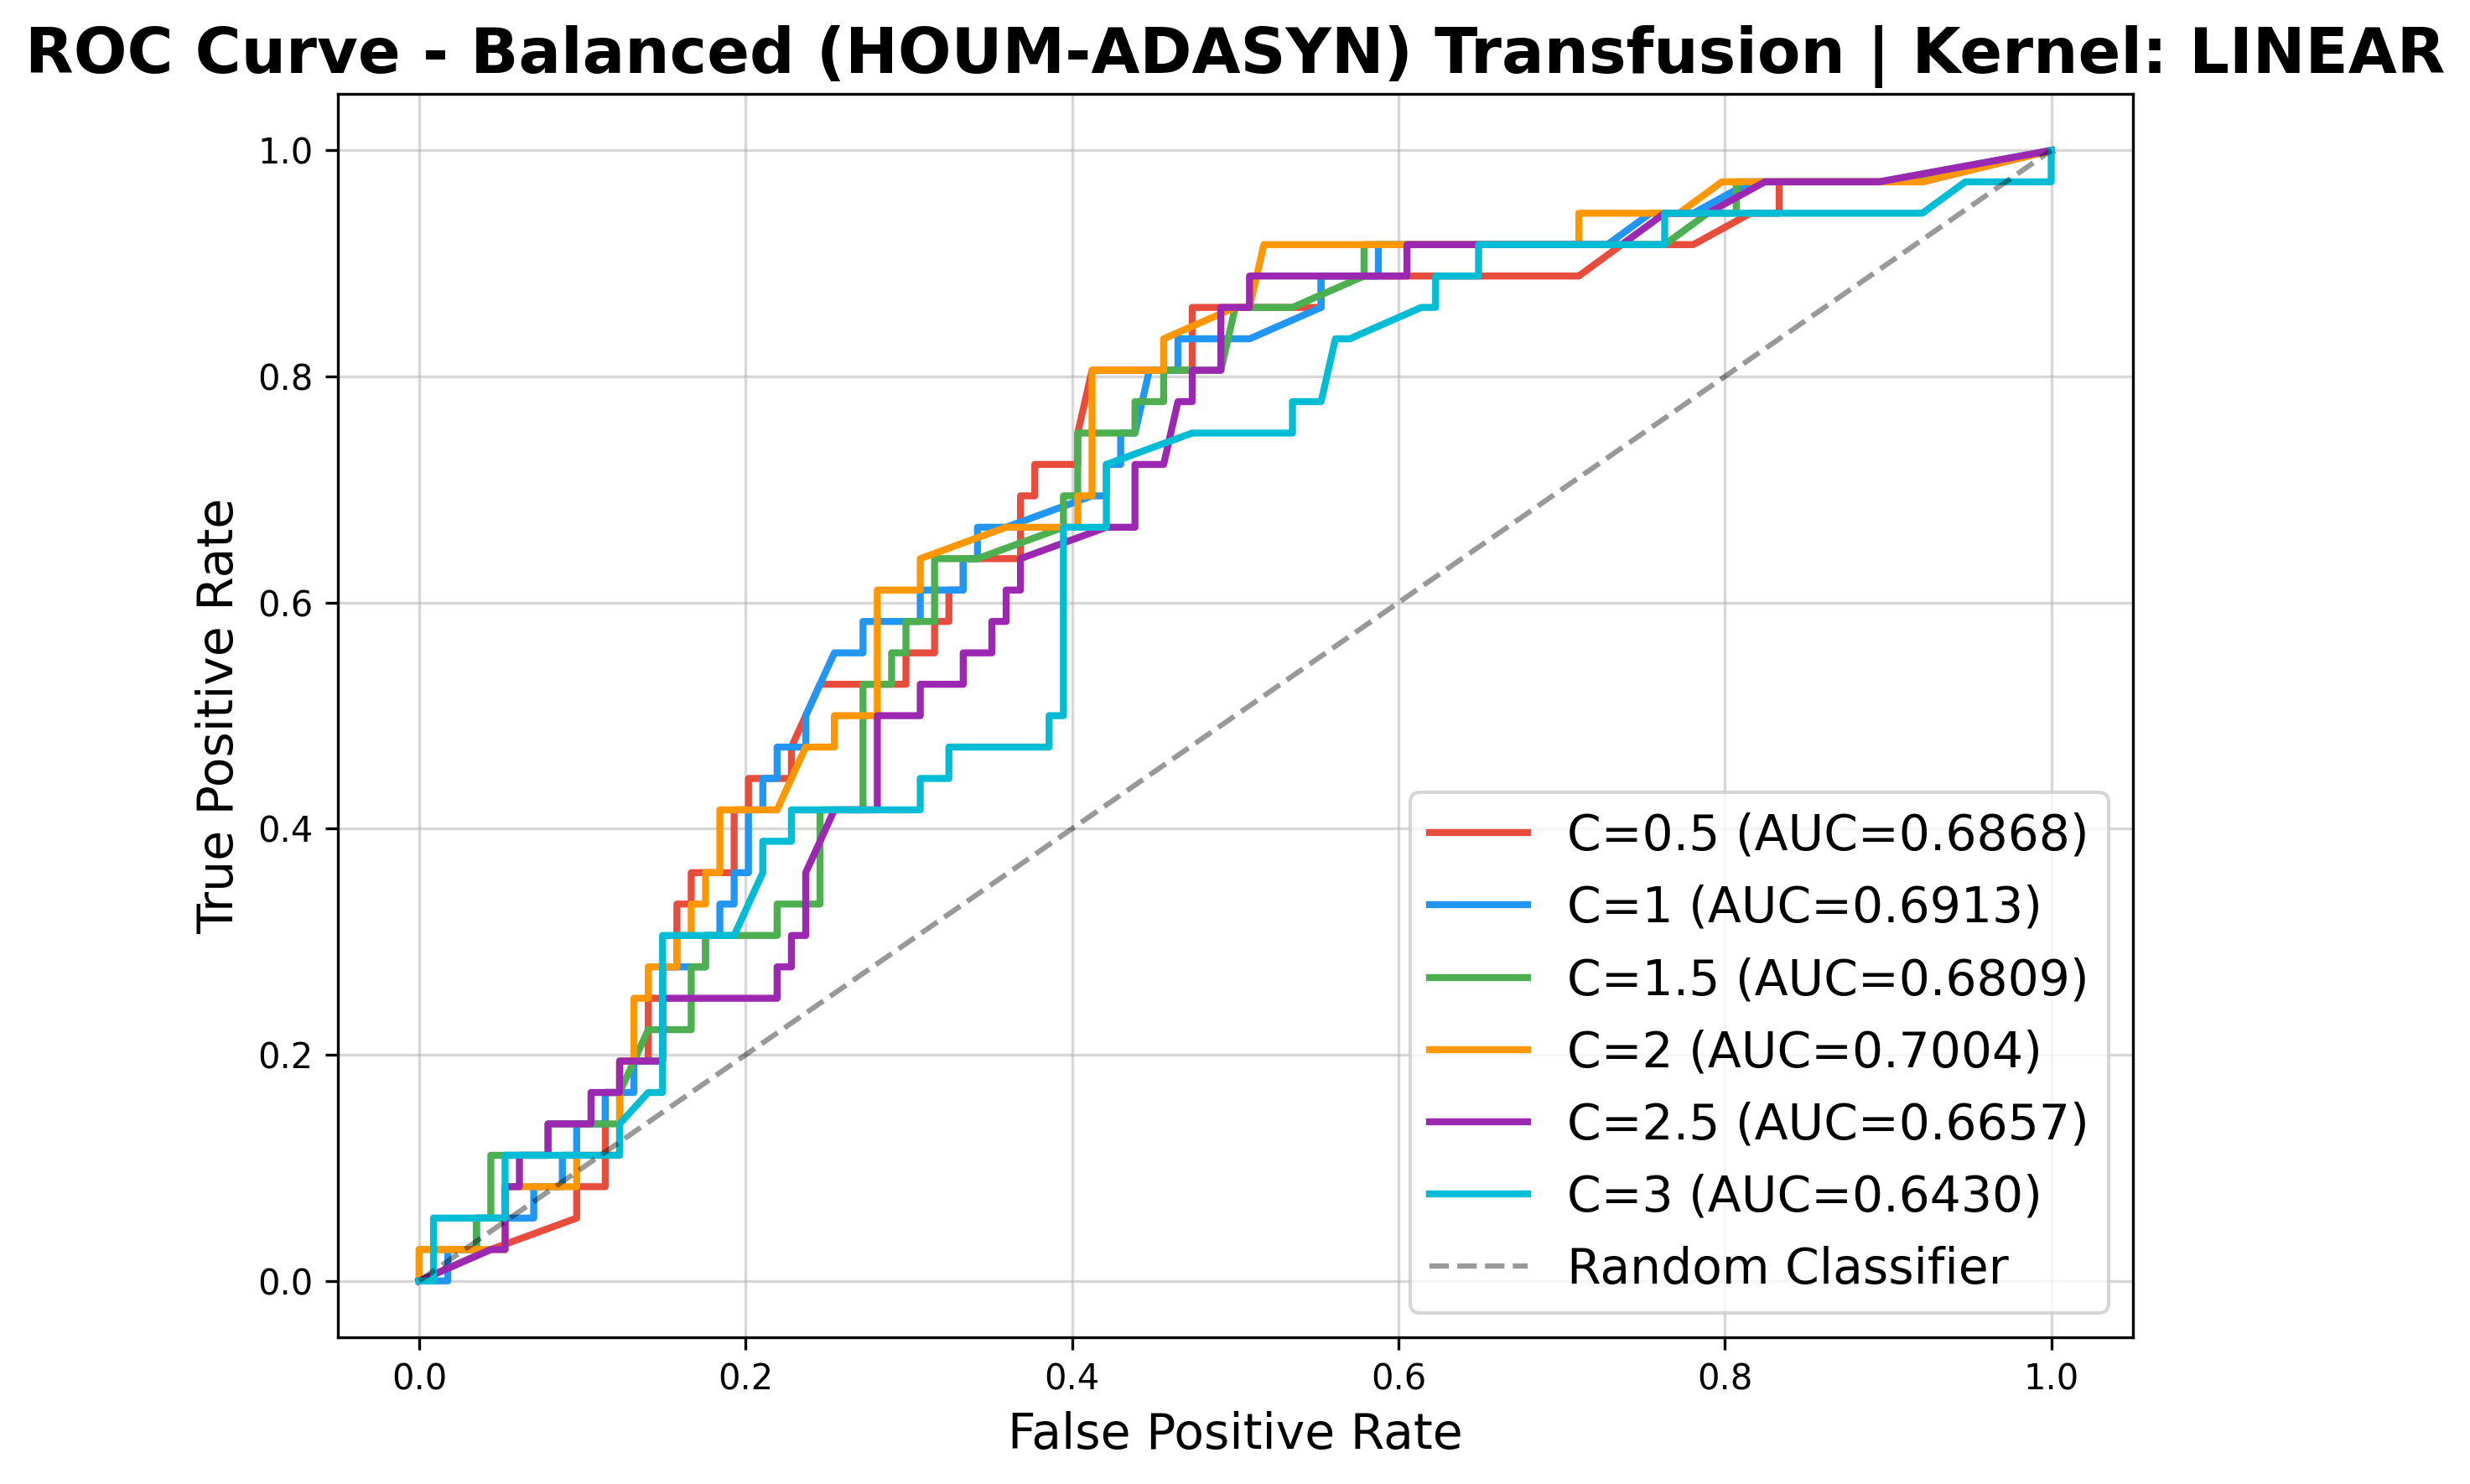
\includegraphics[width=\textwidth]{figure/roc_balanced_transfusion_adasyn_kernel_linear.png}
        \caption{Kernel Linear}
        \label{fig:4.roc_adasyn_transfusion_linear}
    \end{subfigure}
    \hfill
    \begin{subfigure}[b]{0.47\textwidth}
        \centering
        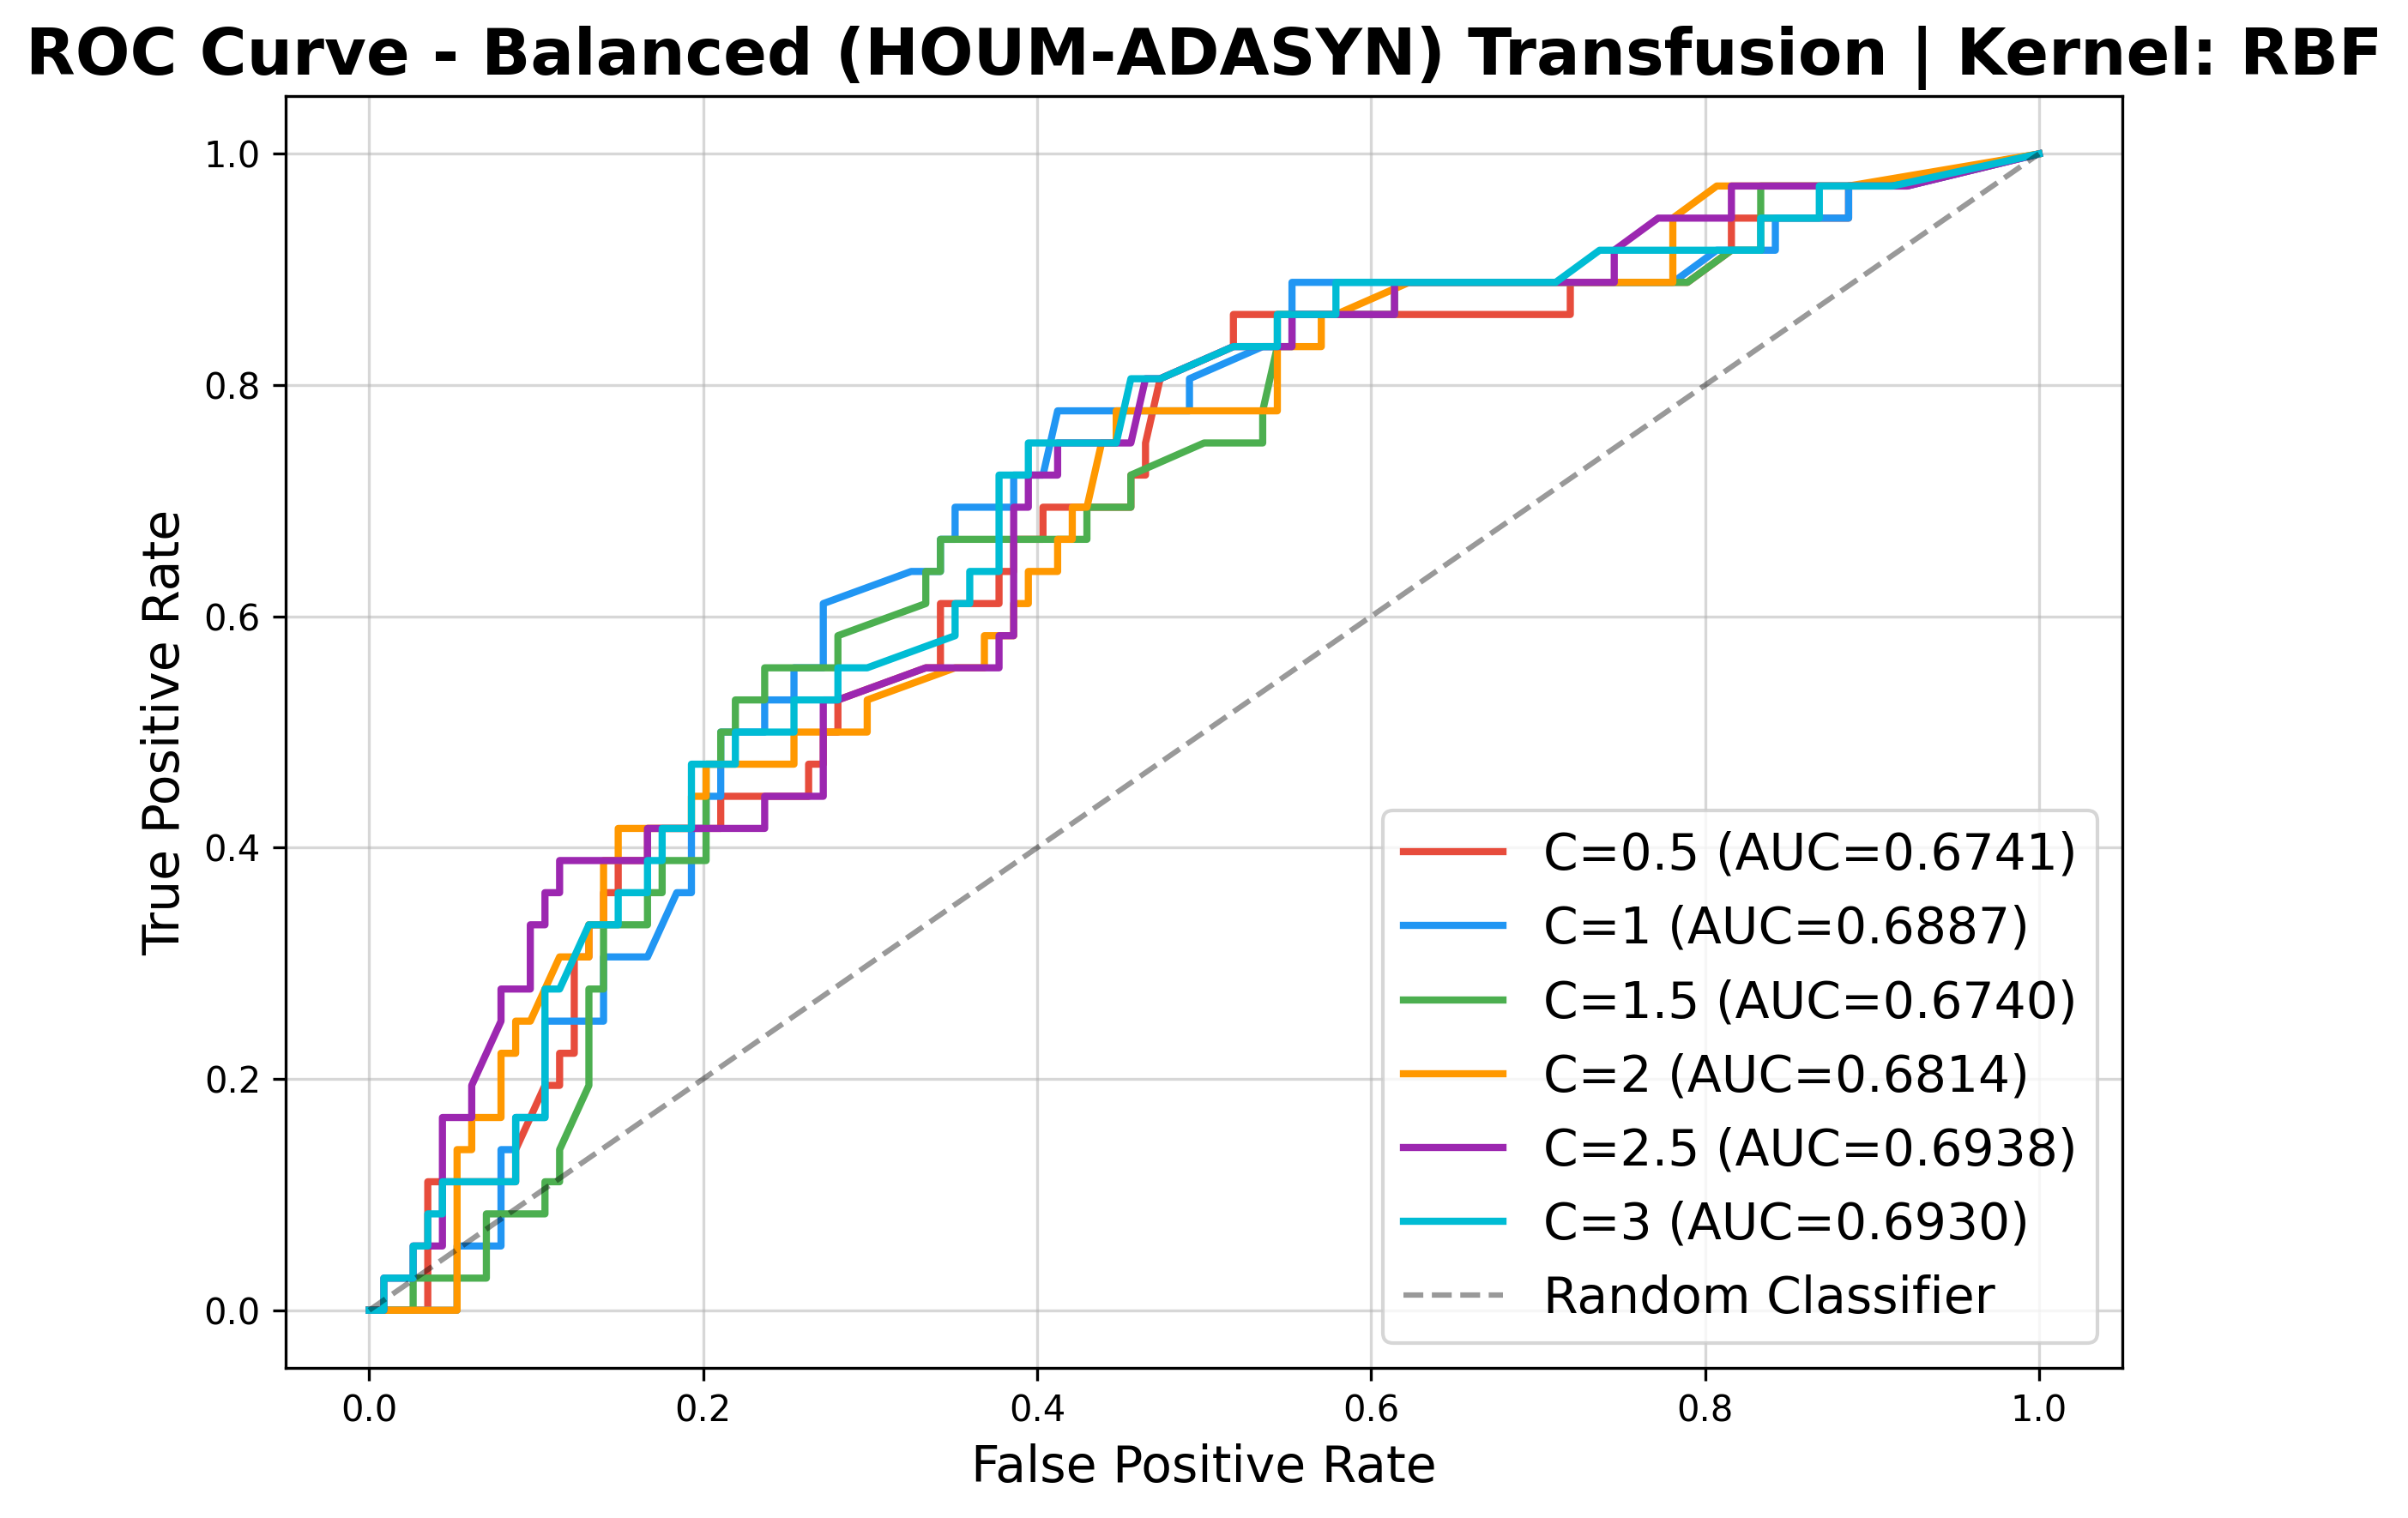
\includegraphics[width=\textwidth]{figure/roc_balanced_transfusion_adasyn_kernel_rbf.png}
        \caption{Kernel RBF}
        \label{fig:4.roc_adasyn_transfusion_rbf}
    \end{subfigure}

    \vspace{0.5em}

    \begin{subfigure}[b]{0.47\textwidth}
        \centering
        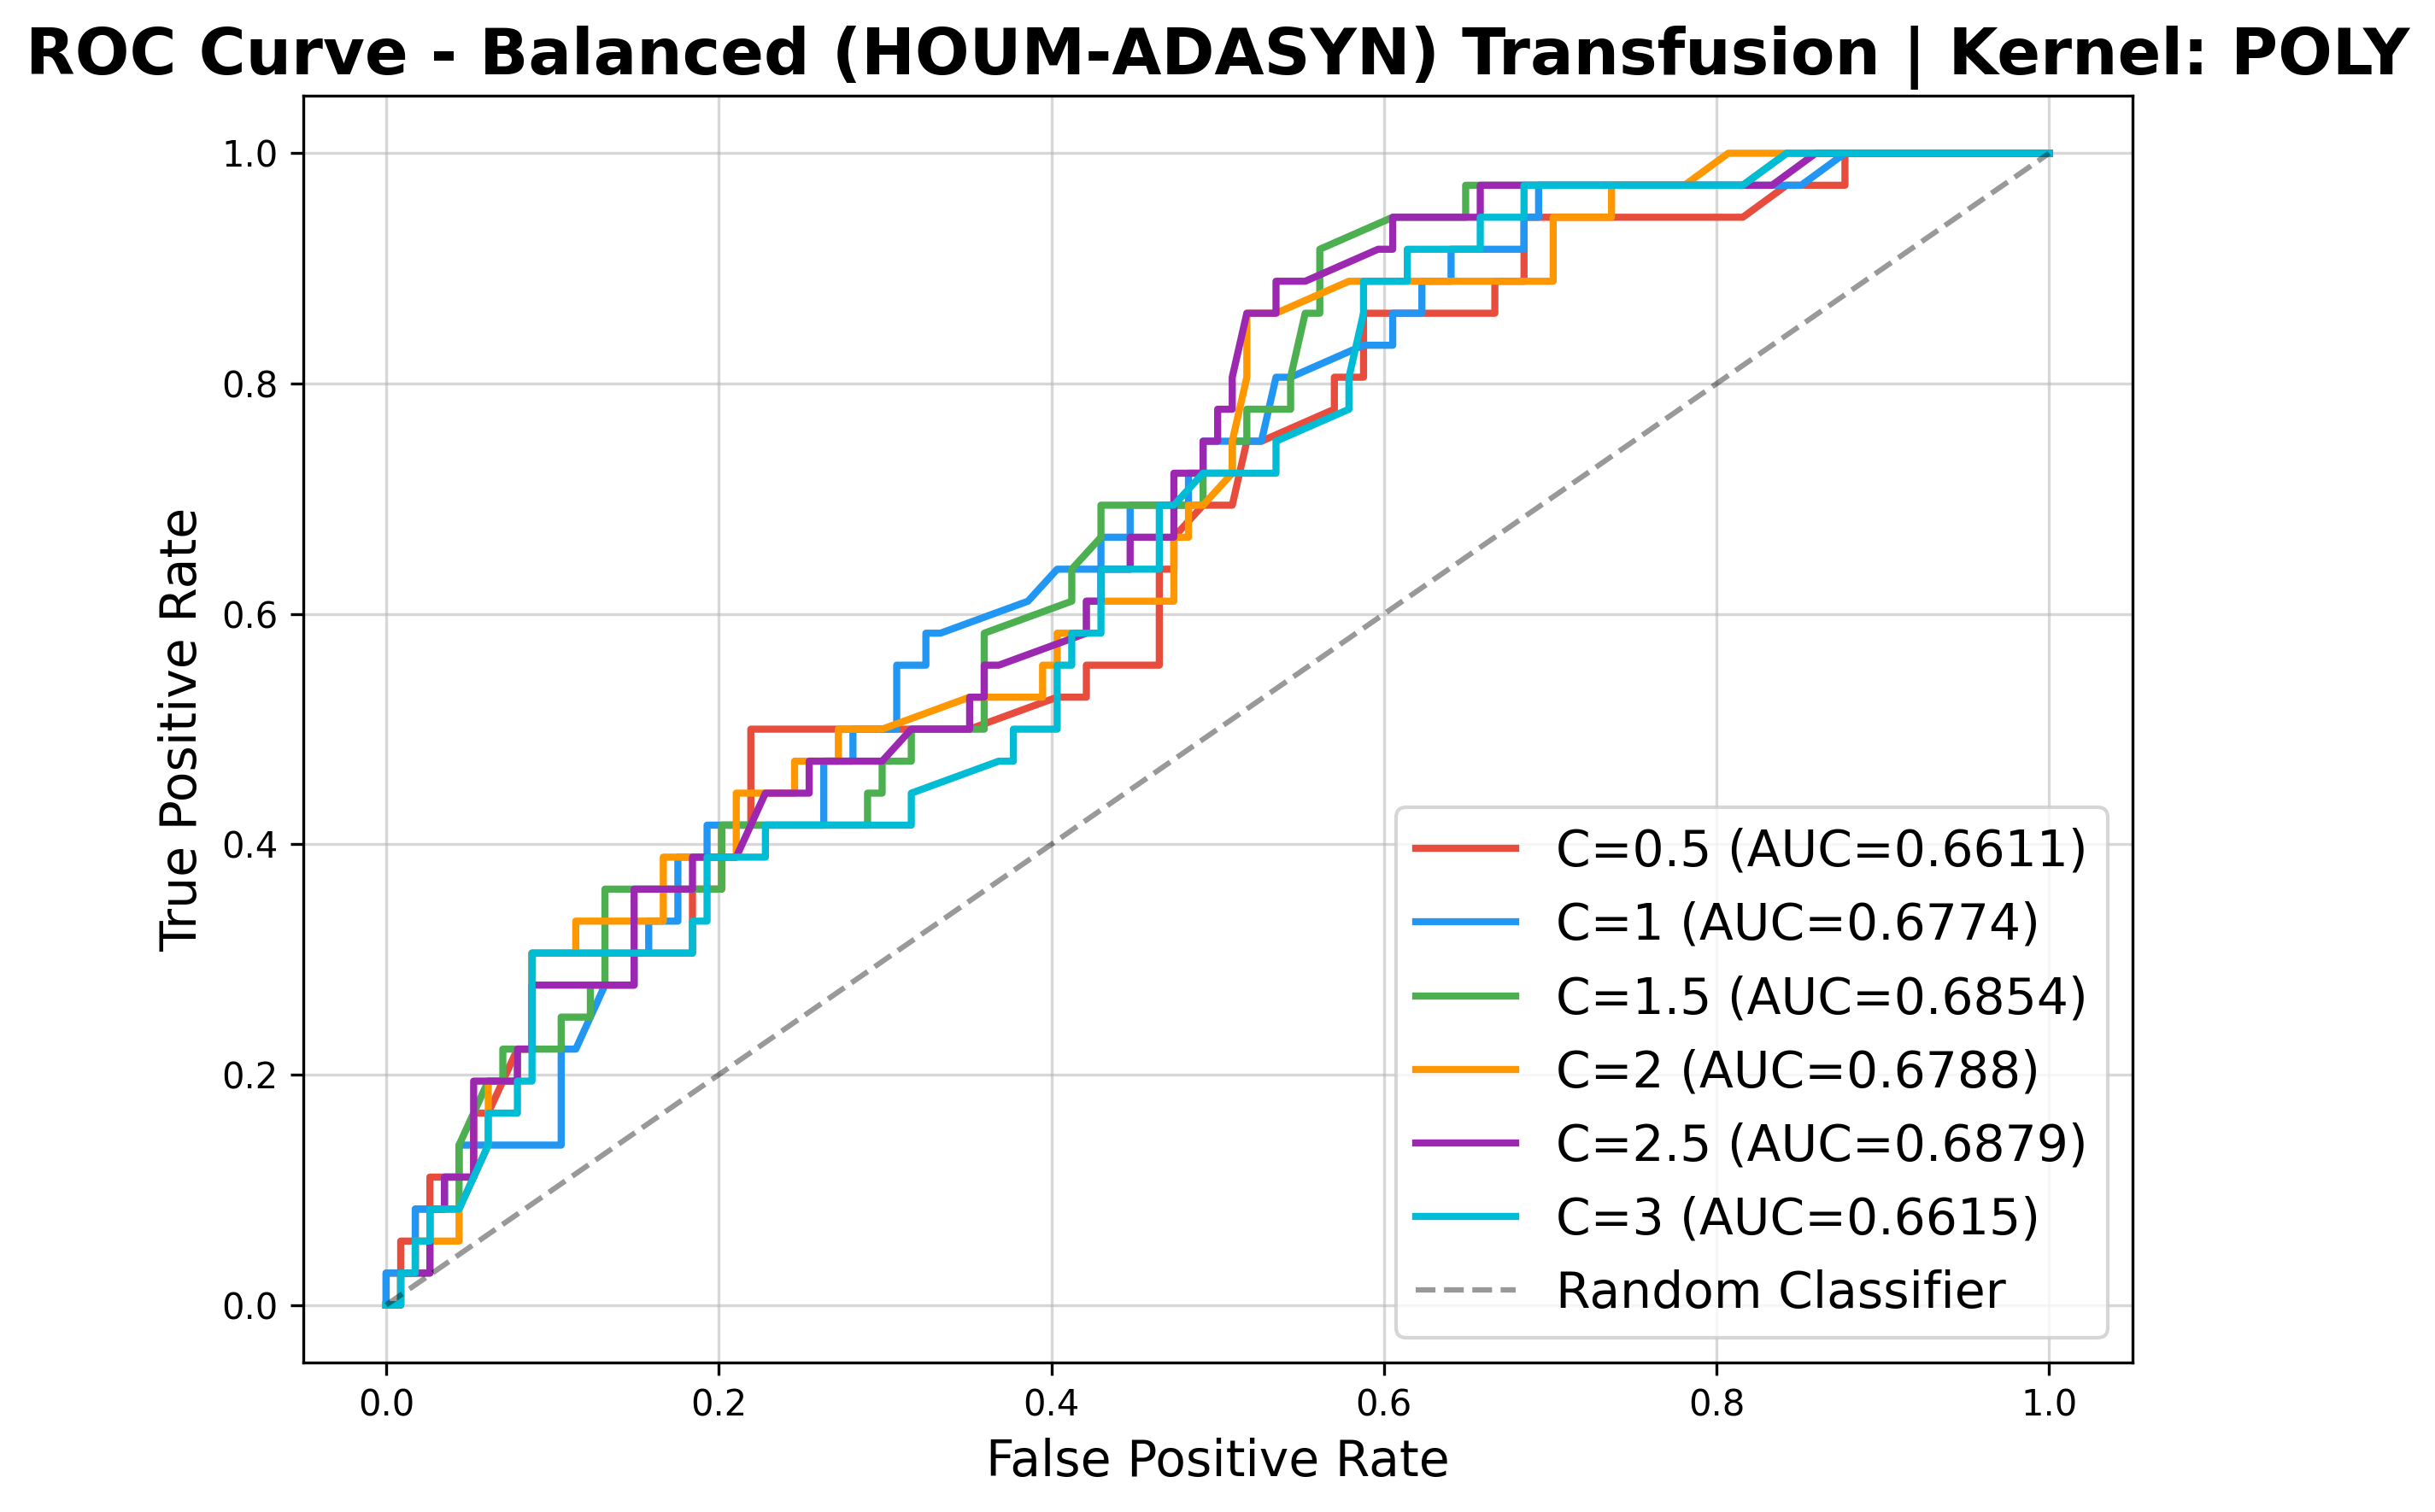
\includegraphics[width=\textwidth]{figure/roc_balanced_transfusion_adasyn_kernel_poly.png}
        \caption{Kernel Polynomial}
        \label{fig:4.roc_adasyn_transfusion_poly}
    \end{subfigure}
    \caption{Kurva ROC HOUM-ADASYN pada Dataset Transfusion}
    \label{fig:4.roc_adasyn_transfusion}
\end{figure}

Berdasarkan Tabel \ref{table:4.adasyn_transfusion}, ROC-AUC tertinggi sebesar 0,7004 dicapai oleh kernel Linear dengan $C$ = 2, sedangkan \textit{Recall} tertinggi 0,7222 diperoleh kernel Linear dengan $C$ = 2,5. G-Mean 0,6623 dan \textit{Precision} 0,3810 dicapai oleh kernel RBF dengan $C$ = 1. Dibandingkan HOUM-SLSMOTE, seluruh nilai puncak HOUM-ADASYN berada di bawah HOUM-SLSMOTE pada \textit{Recall} (0,7222 berbanding 0,7778), \textit{Precision} (0,3810 berbanding 0,4030), dan G-Mean (0,6623 berbanding 0,6977).

\subsubsection{Dataset Glass5} \label{IV.ADASYN_Glass}
Hasil klasifikasi HOUM-ADASYN pada dataset Glass5 untuk seluruh kombinasi kernel dan nilai $C$ ditunjukkan pada Tabel \ref{table:4.adasyn_glass}.

\begin{table}[H]
\centering
\caption{Hasil HOUM-ADASYN pada Dataset Glass5}
\label{table:4.adasyn_glass}
\footnotesize
\begin{tabular}{|l|c|c|c|c|c|c|}
\hline
\textbf{No} & \textbf{Kernel} & \textbf{C} & \textbf{ROC-AUC} & \textbf{\textit{Recall}} & \textbf{\textit{Precision}} & \textbf{G-Mean} \\
\hline
1 & Linear & 0,5 & \textbf{1,0000} & \textbf{1,0000} & \textbf{0,6667} & \textbf{0,9877} \\
\hline
2 & Linear & 1 & \textbf{1,0000} & \textbf{1,0000} & \textbf{0,6667} & \textbf{0,9877} \\
\hline
3 & Linear & 1,5 & \textbf{1,0000} & \textbf{1,0000} & \textbf{0,6667} & \textbf{0,9877} \\
\hline
4 & Linear & 2 & \textbf{1,0000} & \textbf{1,0000} & \textbf{0,6667} & \textbf{0,9877} \\
\hline
5 & Linear & 2,5 & \textbf{1,0000} & \textbf{1,0000} & \textbf{0,6667} & \textbf{0,9877} \\
\hline
6 & Linear & 3 & \textbf{1,0000} & \textbf{1,0000} & \textbf{0,6667} & \textbf{0,9877} \\
\hline
7 & RBF & 0,5 & \textbf{1,0000} & \textbf{1,0000} & \textbf{0,6667} & \textbf{0,9877} \\
\hline
8 & RBF & 1 & \textbf{1,0000} & \textbf{1,0000} & \textbf{0,6667} & \textbf{0,9877} \\
\hline
9 & RBF & 1,5 & \textbf{1,0000} & \textbf{1,0000} & \textbf{0,6667} & \textbf{0,9877} \\
\hline
10 & RBF & 2 & \textbf{1,0000} & \textbf{1,0000} & \textbf{0,6667} & \textbf{0,9877} \\
\hline
11 & RBF & 2,5 & \textbf{1,0000} & \textbf{1,0000} & \textbf{0,6667} & \textbf{0,9877} \\
\hline
12 & RBF & 3 & \textbf{1,0000} & \textbf{1,0000} & \textbf{0,6667} & \textbf{0,9877} \\
\hline
13 & Poly & 0,5 & \textbf{1,0000} & \textbf{1,0000} & \textbf{0,6667} & \textbf{0,9877} \\
\hline
14 & Poly & 1 & \textbf{1,0000} & \textbf{1,0000} & \textbf{0,6667} & \textbf{0,9877} \\
\hline
15 & Poly & 1,5 & \textbf{1,0000} & \textbf{1,0000} & \textbf{0,6667} & \textbf{0,9877} \\
\hline
16 & Poly & 2 & \textbf{1,0000} & \textbf{1,0000} & \textbf{0,6667} & \textbf{0,9877} \\
\hline
17 & Poly & 2,5 & \textbf{1,0000} & \textbf{1,0000} & \textbf{0,6667} & \textbf{0,9877} \\
\hline
18 & Poly & 3 & \textbf{1,0000} & \textbf{1,0000} & \textbf{0,6667} & \textbf{0,9877} \\
\hline
\end{tabular}
\end{table}

Kurva ROC untuk masing-masing kernel pada dataset Glass5 ditunjukkan pada Gambar \ref{fig:4.roc_adasyn_glass}.

\begin{figure}[H]
    \centering
    \begin{subfigure}[b]{0.47\textwidth}
        \centering
        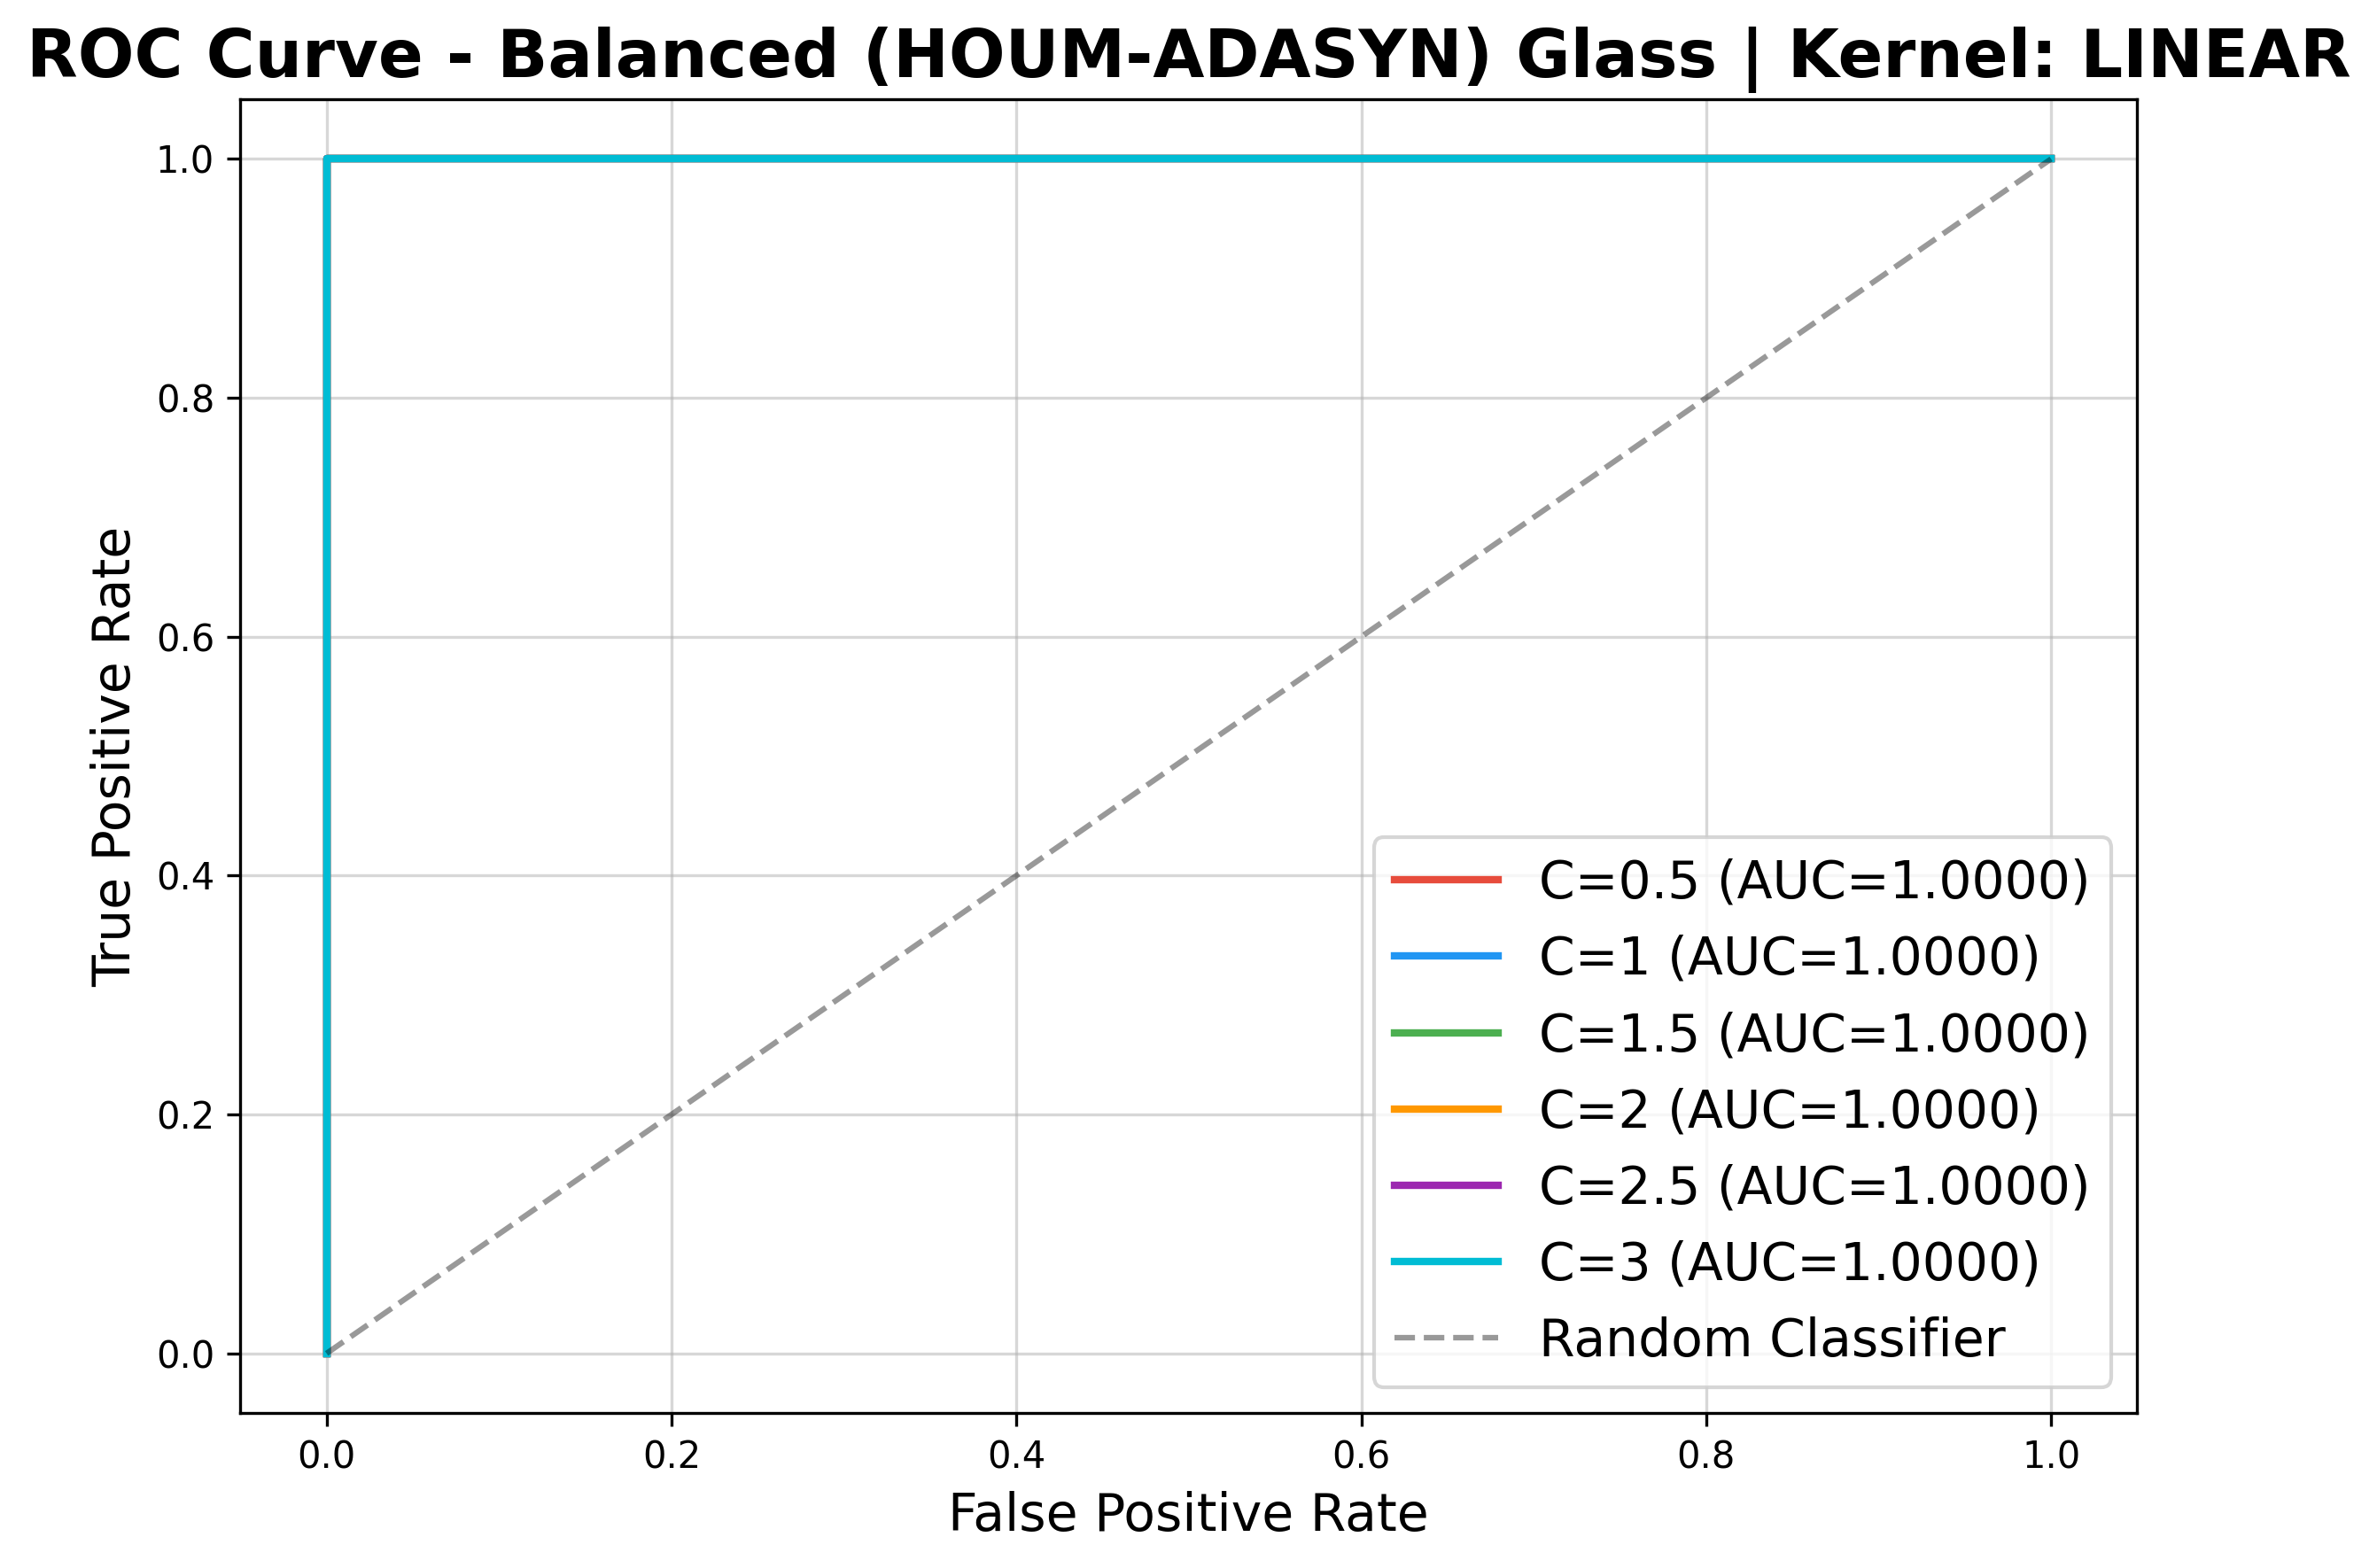
\includegraphics[width=\textwidth]{figure/roc_balanced_glass_adasyn_kernel_linear.png}
        \caption{Kernel Linear}
        \label{fig:4.roc_adasyn_glass_linear}
    \end{subfigure}
    \hfill
    \begin{subfigure}[b]{0.47\textwidth}
        \centering
        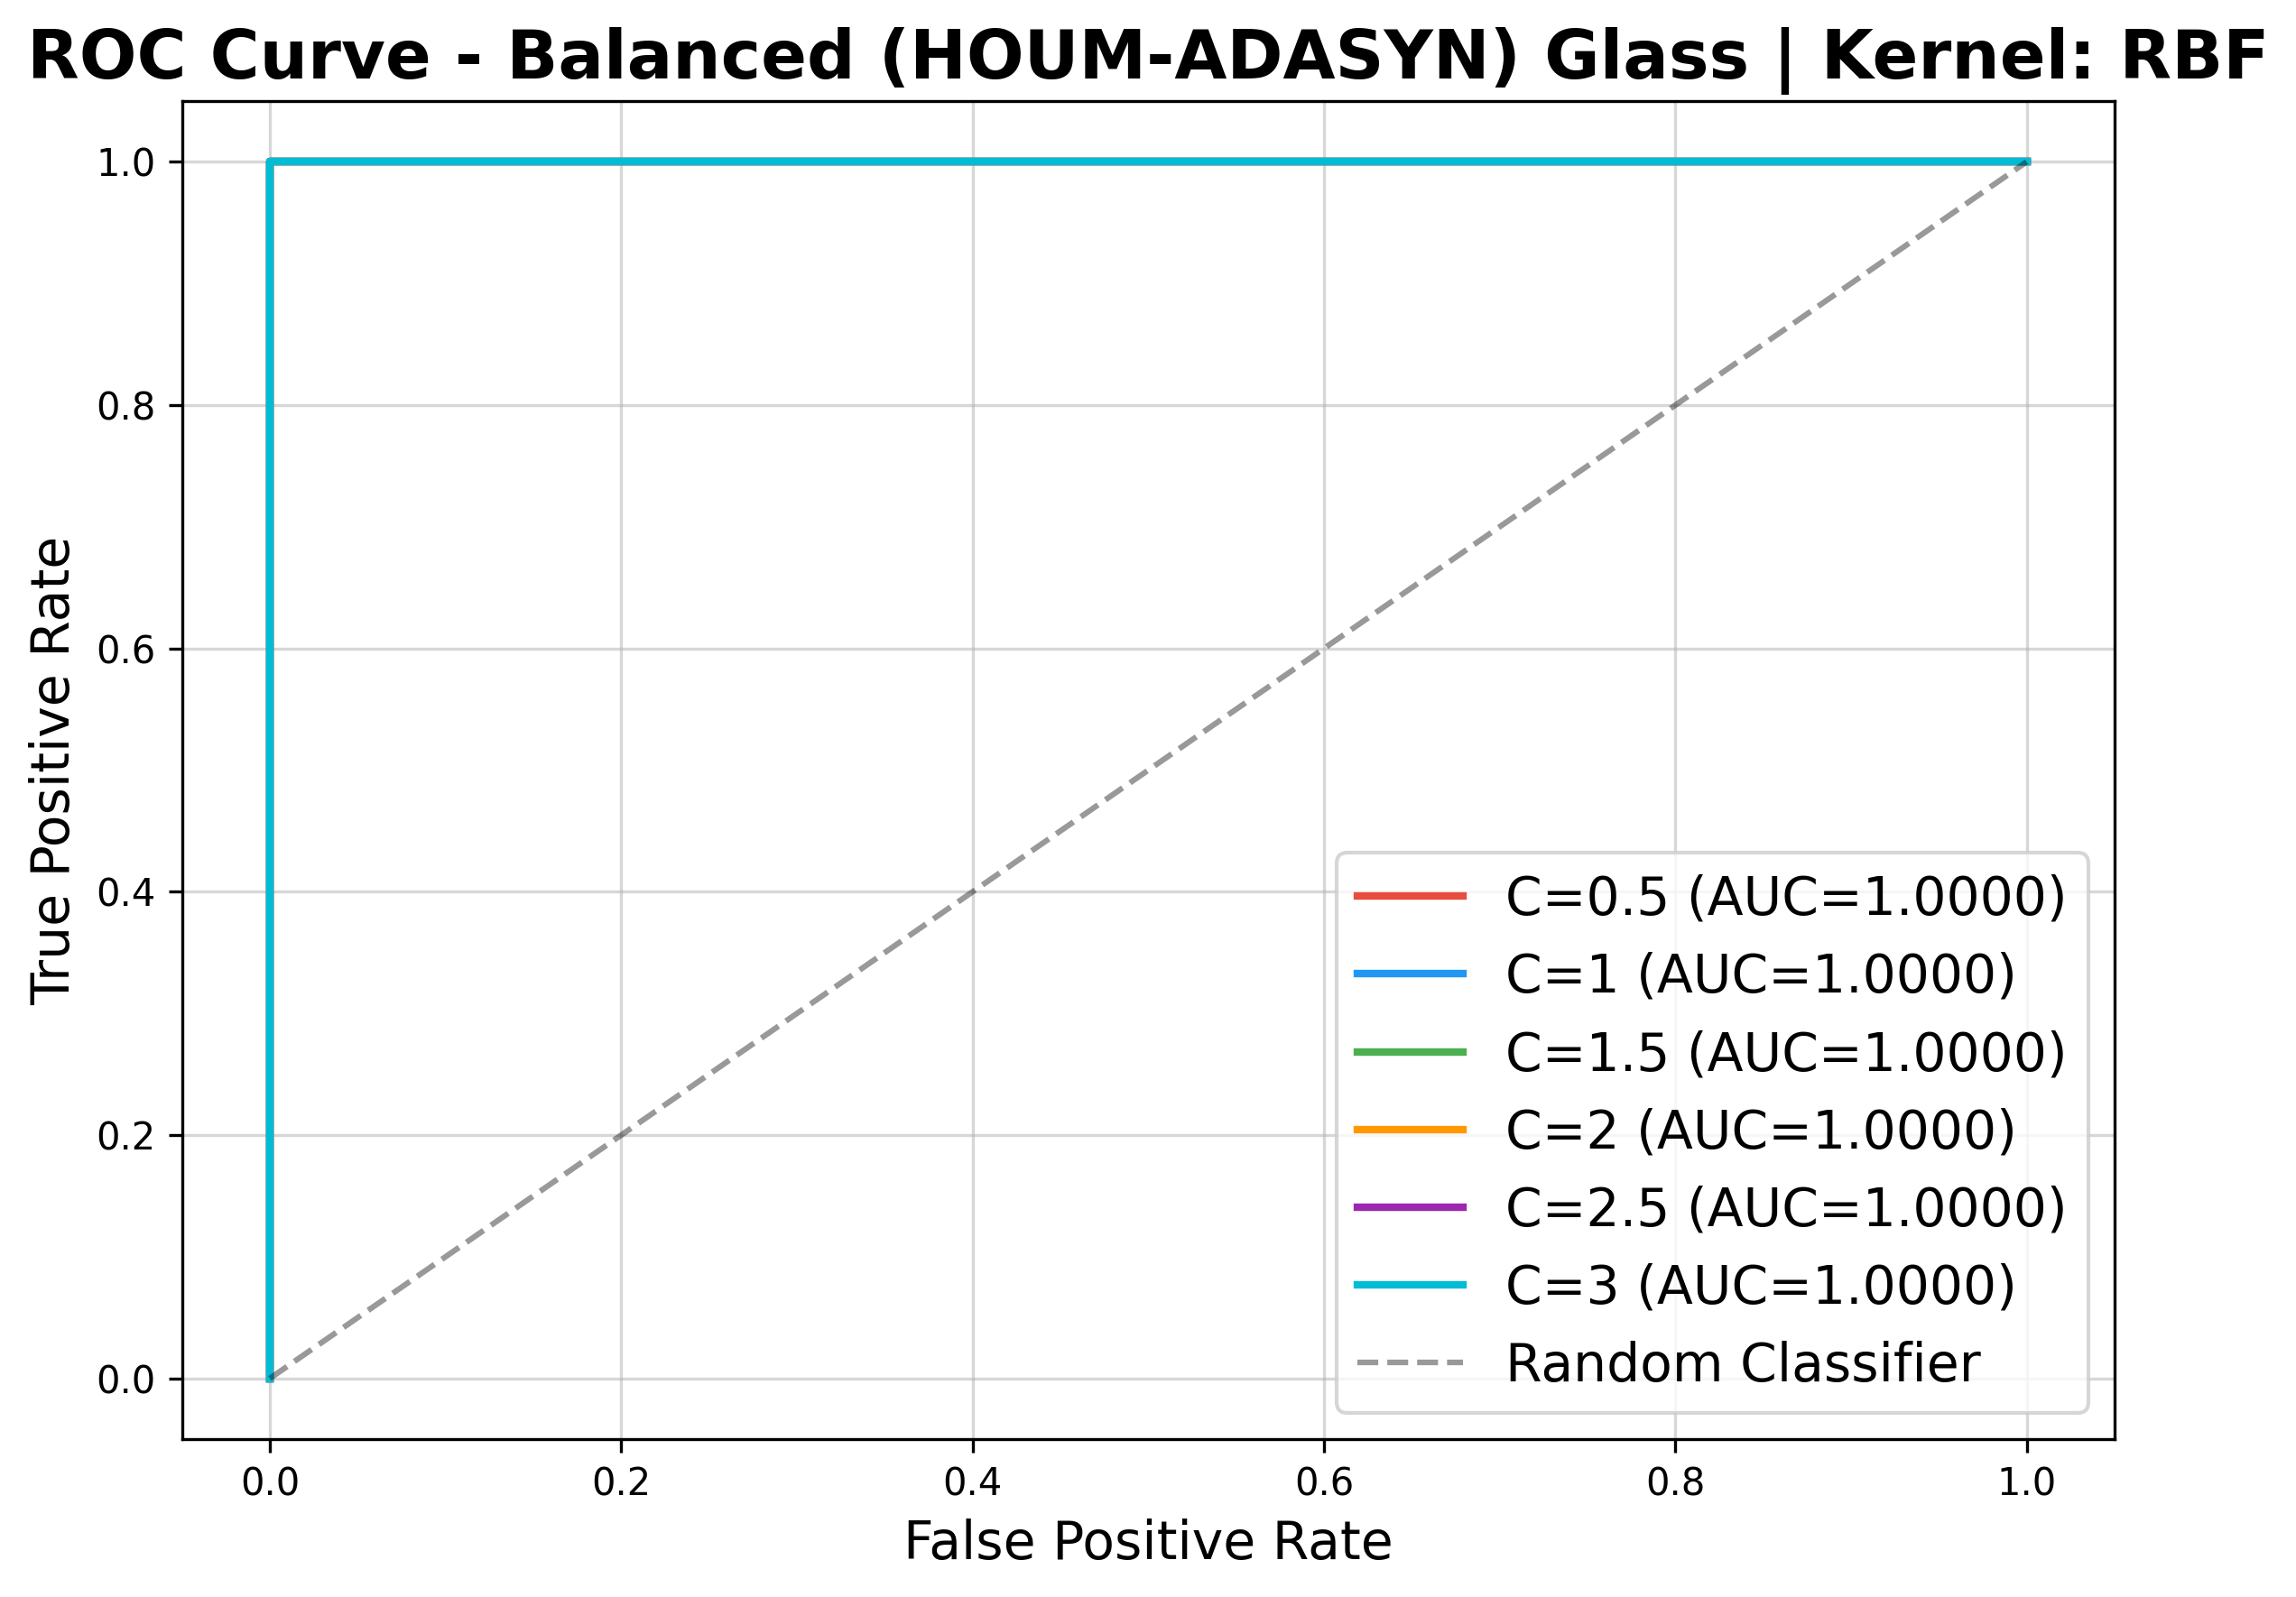
\includegraphics[width=\textwidth]{figure/roc_balanced_glass_adasyn_kernel_rbf.png}
        \caption{Kernel RBF}
        \label{fig:4.roc_adasyn_glass_rbf}
    \end{subfigure}

    \vspace{0.5em}

    \begin{subfigure}[b]{0.47\textwidth}
        \centering
        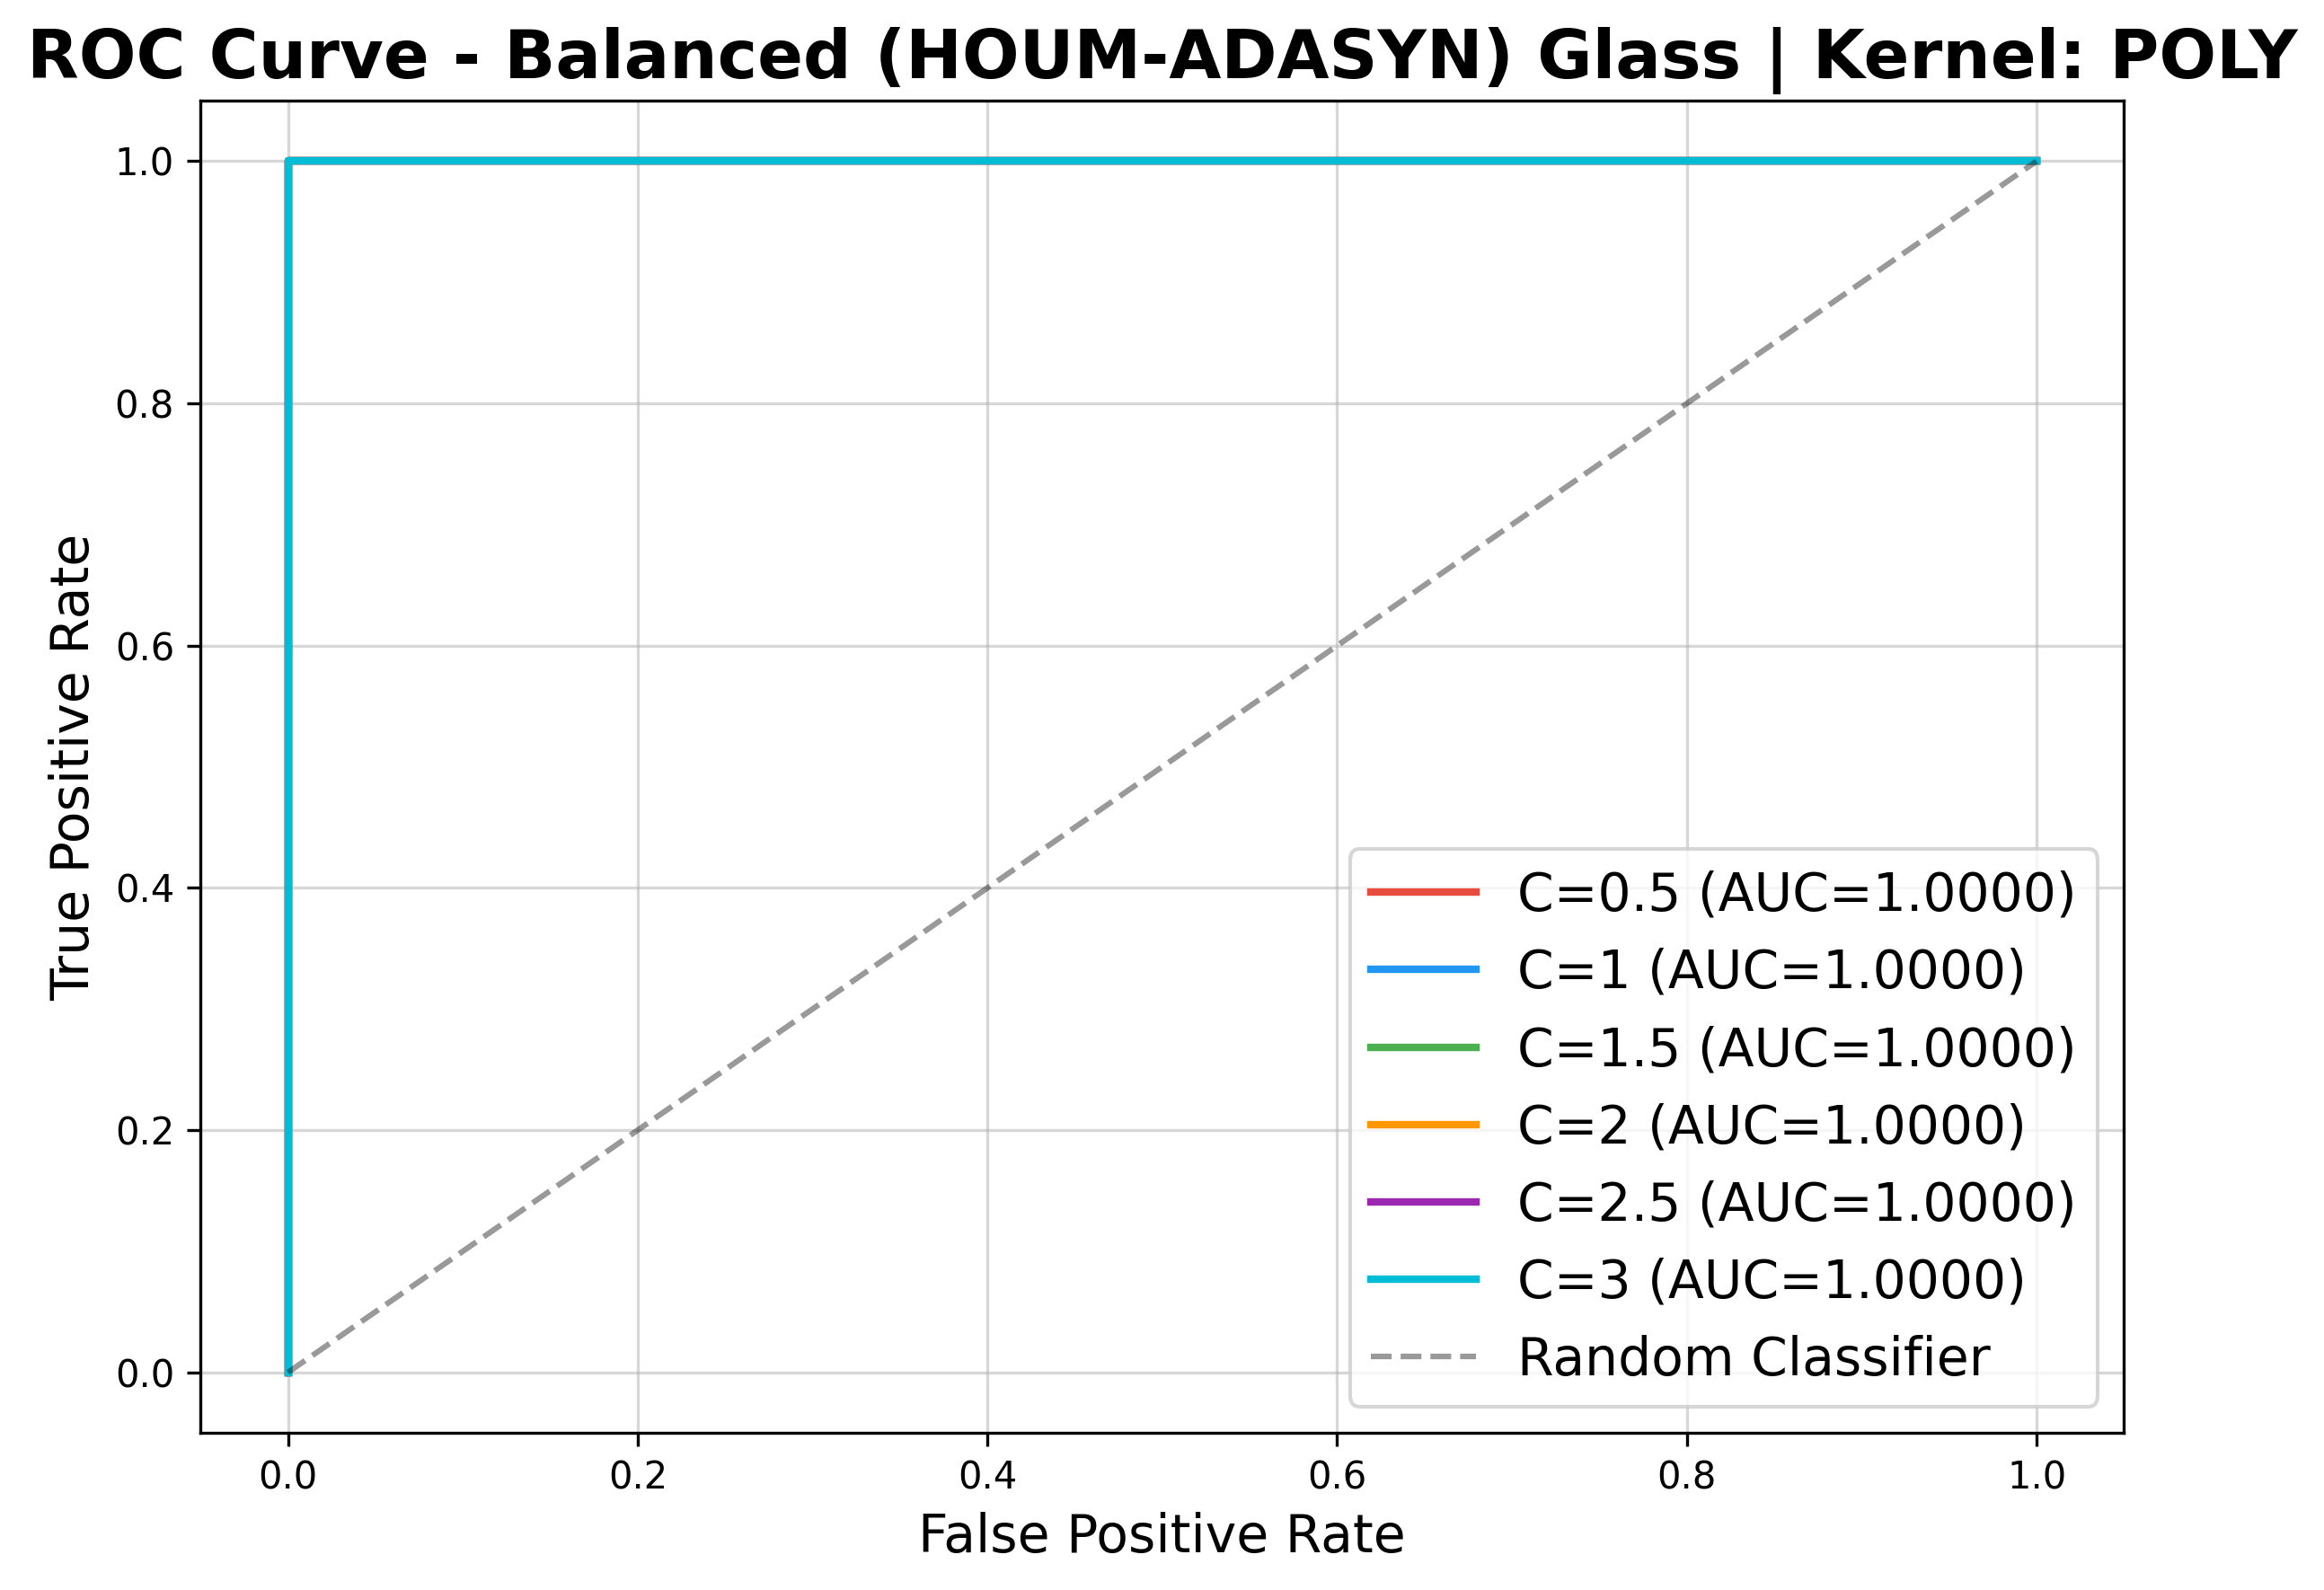
\includegraphics[width=\textwidth]{figure/roc_balanced_glass_adasyn_kernel_poly.png}
        \caption{Kernel Polynomial}
        \label{fig:4.roc_adasyn_glass_poly}
    \end{subfigure}
    \caption{Kurva ROC HOUM-ADASYN pada Dataset Glass5}
    \label{fig:4.roc_adasyn_glass}
\end{figure}

Berdasarkan Tabel \ref{table:4.adasyn_glass}, seluruh kombinasi kernel dan nilai $C$ pada HOUM-ADASYN menghasilkan metrik yang identik, yaitu ROC-AUC 1,0000, \textit{Recall} 1,0000, \textit{Precision} 0,6667, dan G-Mean 0,9877. Variasi konfigurasi SVM tidak memberikan pengaruh terhadap hasil klasifikasi pada dataset ini. Dibandingkan HOUM-SLSMOTE, HOUM-ADASYN mencatat \textit{Precision} lebih tinggi (0,6667 berbanding 0,5000) dan G-Mean lebih tinggi (0,9877 berbanding 0,9753), serta ROC-AUC 1,0000 berbanding 0,9878.

\subsection{Perbandingan Hasil Secara Umum} \label{IV.Perbandingan}
Bagian ini merangkum dan membandingkan performa dari masing-masing metode (\textit{Baseline}, HOUM-SLSMOTE, dan HOUM-ADASYN) pada keempat dataset. Pemilihan konfigurasi didasarkan pada metrik G-Mean sebagai metrik utama karena G-Mean merepresentasikan keseimbangan deteksi kedua kelas. Apabila nilai G-Mean antar konfigurasi berdekatan, \textit{Recall} digunakan sebagai penentu kedua, diikuti ROC-AUC dan \textit{Precision}. Ringkasan konfigurasi ditunjukkan pada Tabel \ref{table:4.ringkasan}.

\begin{table}[H]
\centering
\caption{Ringkasan Performa Tiap Metode pada Setiap Dataset}
\label{table:4.ringkasan}
\footnotesize
\begin{tabular}{|l|l|l|c|c|c|c|}
\hline
\textbf{Dataset} & \textbf{Metode} & \textbf{Konfigurasi} & \textbf{G-Mean} & \textbf{\textit{Recall}} & \textbf{ROC-AUC} & \textbf{\textit{Prec.}} \\
\hline
\multirow{3}{*}{Diabetes} & \textit{Baseline} & -- & 0,7079 & 0,6111 & 0,8194 & 0,6471 \\
\cline{2-7}
 & HOUM-SLS & RBF, $C$=2 & 0,7379 & 0,6481 & 0,8228 & 0,6863 \\
\cline{2-7}
 & HOUM-ADASYN & RBF, $C$=0,5 & 0,7401 & 0,6296 & 0,8093 & 0,7234 \\
\hline
\multirow{3}{*}{Haberman} & \textit{Baseline} & -- & 0,3213 & 0,1250 & 0,5557 & 0,2000 \\
\cline{2-7}
 & HOUM-SLS & Linear, $C$=0,5 & 0,4778 & 0,3750 & 0,5788 & 0,2500 \\
\cline{2-7}
 & HOUM-ADASYN & Linear, $C$=1 & 0,4735 & 0,3125 & 0,5557 & 0,2778 \\
\hline
\multirow{3}{*}{Transfusion} & \textit{Baseline} & -- & 0,6015 & 0,4167 & 0,7523 & 0,5000 \\
\cline{2-7}
 & HOUM-SLS & Linear, $C$=2 & 0,6977 & 0,7500 & 0,7197 & 0,4030 \\
\cline{2-7}
 & HOUM-ADASYN & RBF, $C$=1 & 0,6623 & 0,6667 & 0,6887 & 0,3810 \\
\hline
\multirow{3}{*}{Glass5} & \textit{Baseline} & -- & 0,7071 & 0,5000 & 0,9878 & 1,0000 \\
\cline{2-7}
 & HOUM-SLS & Linear, $C$=0,5 & 0,9753 & 1,0000 & 0,9878 & 0,5000 \\
\cline{2-7}
 & HOUM-ADASYN & Linear, $C$=0,5 & 0,9877 & 1,0000 & 1,0000 & 0,6667 \\
\hline
\end{tabular}
\end{table}

Berdasarkan Tabel \ref{table:4.ringkasan}, HOUM-ADASYN terpilih pada dataset Diabetes (G-Mean 0,7401) dan Glass5 (G-Mean 0,9877), sedangkan HOUM-SLSMOTE terpilih pada dataset Haberman (G-Mean 0,4778) dan Transfusion (G-Mean 0,6977). Seluruh konfigurasi terpilih menghasilkan G-Mean dan \textit{Recall} yang melebihi \textit{baseline}, meskipun pada dataset Transfusion dan Glass5 \textit{Precision} menurun dari \textit{baseline}. Kernel RBF dominan pada dataset Diabetes, kernel Linear dominan pada Haberman dan Transfusion, sedangkan pada Glass5 seluruh kernel pada HOUM-ADASYN menghasilkan nilai yang identik.

\section{Pembahasan Penelitian} \label{IV.Pembahasan}

\subsection{Analisis Dampak Penerapan HOUM pada Data Tidak Seimbang} \label{IV.Dampak_HOUM}
Penerapan HOUM mengubah distribusi data \textit{training} melalui dua tahap. Pertama, komponen \textit{undersampling} SVM menghapus sampel kelas mayoritas yang berada jauh dari \textit{decision boundary}. Kedua, komponen \textit{oversampling} (Safe-Level SMOTE atau ADASYN) menambahkan sampel sintetis kelas minoritas. Perubahan distribusi ini memengaruhi keempat metrik evaluasi dengan pola yang berbeda pada setiap dataset, sebagaimana disajikan pada Tabel \ref{table:4.dampak_houm}. \par

\begin{table}[H]
\centering
\caption{Perbandingan Metrik Evaluasi \textit{Baseline} dan HOUM pada Keempat Dataset}
\label{table:4.dampak_houm}
\footnotesize
\begin{tabular}{|l|l|c|c|c|}
\hline
\textbf{Dataset} & \textbf{Metrik} & \textbf{\textit{Baseline}} & \textbf{HOUM-SLS} & \textbf{HOUM-ADASYN} \\
\hline
\multirow{4}{*}{Diabetes} & \textit{Recall} & 0,6111 & \textbf{0,6481} & 0,6296 \\
 & \textit{Precision} & 0,6471 & 0,6863 & \textbf{0,7234} \\
 & G-Mean & 0,7079 & 0,7379 & \textbf{0,7401} \\
 & ROC-AUC & 0,8194 & \textbf{0,8228} & 0,8093 \\
\hline
\multirow{4}{*}{Haberman} & \textit{Recall} & 0,1250 & \textbf{0,3750} & 0,3125 \\
 & \textit{Precision} & 0,2000 & 0,2500 & \textbf{0,2778} \\
 & G-Mean & 0,3213 & \textbf{0,4778} & 0,4735 \\
 & ROC-AUC & 0,5557 & \textbf{0,5788} & 0,5557 \\
\hline
\multirow{4}{*}{Transfusion} & \textit{Recall} & 0,4167 & \textbf{0,7500} & 0,6667 \\
 & \textit{Precision} & \textbf{0,5000} & 0,4030 & 0,3810 \\
 & G-Mean & 0,6015 & \textbf{0,6977} & 0,6623 \\
 & ROC-AUC & \textbf{0,7523} & 0,7197 & 0,6887 \\
\hline
\multirow{4}{*}{Glass5} & \textit{Recall} & 0,5000 & \textbf{1,0000} & \textbf{1,0000} \\
 & \textit{Precision} & \textbf{1,0000} & 0,5000 & 0,6667 \\
 & G-Mean & 0,7071 & 0,9753 & \textbf{0,9877} \\
 & ROC-AUC & 0,9878 & 0,9878 & \textbf{1,0000} \\
\hline
\end{tabular}
\end{table}

\subsubsection{Perubahan Nilai Metrik Evaluasi}
Penerapan HOUM menghasilkan dua pola perubahan metrik yang berbeda. Pola pertama terjadi pada dataset Diabetes (rasio 1:1,87, delapan fitur), di mana seluruh metrik naik secara bersamaan. \textit{Recall} naik dari 0,6111 ke 0,6481 (HOUM-SLS) dan 0,6296 (HOUM-ADASYN); \textit{Precision} naik ke 0,6863 dan 0,7234; G-Mean naik ke 0,7379 dan 0,7401. Kenaikan ini terjadi karena rasio ketidakseimbangan yang rendah dan delapan fitur memberikan ruang pemisahan yang cukup. HOUM menghapus sampel mayoritas tidak informatif melalui SVM dan menambahkan sampel minoritas sintetis tanpa menciptakan tumpang tindih baru yang berarti, sehingga batas keputusan bergeser menguntungkan kelas minoritas tanpa mengorbankan akurasi pada kelas mayoritas.

Pola kedua terjadi pada dataset Transfusion (rasio 1:3,20, empat fitur), di mana \textit{Recall} dan G-Mean naik signifikan tetapi \textit{Precision} dan ROC-AUC turun. \textit{Recall} naik dari 0,4167 ke 0,7500 (HOUM-SLS) dan 0,6667 (HOUM-ADASYN), namun \textit{Precision} turun dari 0,5000 ke 0,4030 dan 0,3810, serta ROC-AUC turun dari 0,7523 ke 0,7197 dan 0,6887. \textit{Trade-off} ini muncul karena ketidakseimbangan yang tinggi memaksa batas keputusan bergeser cukup jauh untuk menangkap lebih banyak sampel kelas minoritas. Pergeseran ini memperluas area prediksi positif sehingga \textit{false positive} bertambah, yang secara langsung menekan \textit{Precision} dan ROC-AUC. Semakin tinggi rasio ketidakseimbangan, semakin besar pergeseran batas yang diperlukan, dan semakin besar penurunan \textit{Precision} sebagai konsekuensinya.

Dataset Haberman (rasio 1:2,78, tiga fitur) berada di antara kedua pola tersebut. Seluruh metrik naik dari \textit{baseline}, tetapi nilai absolutnya tetap rendah: \textit{Recall} dari 0,1250 ke 0,3750 (HOUM-SLS), G-Mean ke 0,4778, dan ROC-AUC hanya mencapai 0,5788. Kenaikan terjadi karena HOUM mengurangi bias terhadap kelas mayoritas, namun ruang fitur yang hanya tiga dimensi menyebabkan tumpang tindih antar kelas pada \textit{baseline}, ROC-AUC 0,5557 hampir setara \textit{random classifier}. Dalam kondisi ini, sampel sintetis yang ditambahkan oleh \textit{oversampling} jatuh di area yang sudah tercampur antar kelas, sehingga tidak cukup membantu model membentuk batas keputusan yang jelas antara pasien yang bertahan dan tidak bertahan hidup. \par

Dataset Glass5 (rasio 1:22,78, sembilan fitur) menunjukkan pola ketiga. \textit{Recall} naik dari 0,5000 menjadi 1,0000 pada kedua metode, yang berarti seluruh sampel minoritas terdeteksi. \textit{Precision} turun dari 1,0000 (\textit{baseline}) menjadi 0,5000 (HOUM-SLS) dan 0,6667 (HOUM-ADASYN). G-Mean meningkat dari 0,7071 menjadi 0,9753 (HOUM-SLS) dan 0,9877 (HOUM-ADASYN). ROC-AUC yang sudah tinggi pada \textit{baseline} (0,9878) tetap bertahan atau meningkat ke 1,0000 (HOUM-ADASYN). Peningkatan \textit{Recall} yang besar terjadi karena penyeimbangan data memberikan cukup sampel minoritas kepada model untuk dipelajari, yang sebelumnya hanya tersedia 9 sampel. Penurunan \textit{Precision} terjadi karena bertambahnya jumlah prediksi positif seiring dengan peningkatan \textit{Recall}, sehingga beberapa \textit{false positive} muncul. Sembilan fitur pada Glass5 memberikan ruang pemisahan yang baik sehingga data sintetis tidak menciptakan tumpang tindih berarti, berbeda dengan Haberman yang memiliki ruang fitur terbatas. \par

\subsubsection{Mekanisme Kerja HOUM}
Komponen \textit{undersampling} SVM pada HOUM menghapus sampel kelas mayoritas yang berada jauh dari \textit{decision boundary}. Proses ini mengurangi dominasi kelas mayoritas tanpa menghilangkan sampel informatif di sekitar batas keputusan, sehingga model dapat mempelajari perbedaan antar kelas dengan proporsi yang lebih seimbang. Pada sisi \textit{oversampling}, Safe-Level SMOTE menempatkan sampel sintetis di posisi aman berdasarkan rasio keamanan terhadap tetangga dari kelas yang sama. Pendekatan ini menjauhkan sampel sintetis dari area yang didominasi kelas mayoritas, sehingga risiko menghasilkan sampel bising (\textit{noise}) yang membingungkan model menjadi kecil. Sebaliknya, ADASYN mengalokasikan lebih banyak sampel sintetis di area yang sulit diklasifikasikan, yaitu di sekitar batas keputusan antar kelas. Pendekatan ini mendorong model untuk membentuk batas keputusan yang lebih tegas di area kritis, namun rentan terhadap \textit{noise} apabila area tersebut sudah memiliki tumpang tindih kelas yang tinggi. Perbedaan mekanisme ini menjelaskan mengapa HOUM-SLSMOTE cenderung menghasilkan \textit{Recall} yang lebih tinggi pada seluruh dataset, sementara HOUM-ADASYN cenderung unggul pada \textit{Precision} di dataset tertentu. \par
\subsection{Analisis Pengaruh Metode \textit{Oversampling}} \label{IV.Pengaruh_Oversampling}
Bagian ini menganalisis pengaruh penggunaan teknik \textit{oversampling} yang berbeda (Safe-Level SMOTE dan ADASYN) pada metode HOUM terhadap kinerja klasifikasi. Perbandingan merujuk pada Tabel \ref{table:4.dampak_houm}. \par

\subsubsection{Perbandingan Performa antar Metode}
Berdasarkan Tabel \ref{table:4.dampak_houm}, HOUM-SLSMOTE mencatat \textit{Recall} yang selalu di atas atau setara dengan HOUM-ADASYN pada keempat dataset: 0,6481 berbanding 0,6296 pada Diabetes, 0,3750 berbanding 0,3125 pada Haberman, 0,7500 berbanding 0,6667 pada Transfusion, dan 1,0000 pada kedua metode di Glass5. Selisih \textit{Recall} terbesar terjadi pada Transfusion (0,0833), yang menunjukkan bahwa perbedaan pengaruh kedua teknik \textit{oversampling} semakin terlihat pada dataset dengan rasio ketidakseimbangan yang tinggi, kecuali pada Glass5 yang mencapai \textit{Recall} maksimum di kedua metode. \par

Pada metrik G-Mean, HOUM-ADASYN sedikit mengungguli HOUM-SLSMOTE pada dataset Diabetes (0,7401 berbanding 0,7379) dan Glass5 (0,9877 berbanding 0,9753). Pada Haberman dan Transfusion, HOUM-SLSMOTE mencatat G-Mean yang lebih tinggi (0,4778 berbanding 0,4735 pada Haberman; 0,6977 berbanding 0,6623 pada Transfusion). Pola ini menunjukkan bahwa HOUM-SLSMOTE mampu menjaga keseimbangan deteksi kedua kelas secara lebih konsisten di berbagai karakteristik dataset, sementara HOUM-ADASYN unggul pada dataset dengan jumlah fitur yang lebih banyak (Diabetes dan Glass5). \par

Untuk \textit{Precision}, HOUM-ADASYN mencatat nilai yang lebih tinggi pada Diabetes (0,7234 berbanding 0,6863) dan Haberman (0,2778 berbanding 0,2500), sedangkan pada Transfusion, \textit{Precision} HOUM-SLSMOTE di atas HOUM-ADASYN (0,4030 berbanding 0,3810). Perbedaan \textit{Precision} ini berkaitan langsung dengan cara masing-masing teknik menyebarkan sampel sintetis di ruang fitur. \par

\subsubsection{Penyebab Perbedaan Performa}
Perbedaan performa kedua teknik \textit{oversampling} disebabkan oleh mekanisme penempatan sampel sintetis yang berbeda secara mendasar. Safe-Level SMOTE menghitung rasio keamanan (\textit{safe level ratio}) setiap sampel minoritas berdasarkan proporsi tetangga yang berasal dari kelas yang sama. Sampel sintetis ditempatkan semakin dekat dengan sampel yang memiliki rasio keamanan tinggi, yaitu sampel yang dikelilingi oleh sesama kelas minoritas. Mekanisme ini mencegah pembentukan sampel sintetis di area yang didominasi kelas mayoritas, sehingga batas keputusan yang terbentuk setelah penyeimbangan menjadi jelas dan tidak bising. Dampaknya, model mampu mendeteksi lebih banyak sampel minoritas (\textit{Recall} tinggi) tanpa mengorbankan kestabilan prediksi secara keseluruhan. \par

ADASYN menghitung bobot distribusi setiap sampel minoritas berdasarkan proporsi tetangga dari kelas mayoritas. Sampel minoritas yang dikelilingi lebih banyak oleh kelas mayoritas (area batas keputusan) mendapatkan alokasi sampel sintetis yang lebih besar. Pendekatan ini mendorong batas keputusan untuk bergeser ke area yang sulit, sehingga model dapat memisahkan kelas dengan lebih tegas di area kritis. Pada dataset Diabetes yang memiliki delapan fitur dan batas kelas yang relatif jelas, fokus ADASYN pada area batas justru memperkuat batasan model sehingga \textit{Precision} dan G-Mean tercatat lebih tinggi. Namun, pada dataset dengan tumpang tindih kelas yang tinggi seperti Haberman dan Transfusion, penambahan sampel sintetis di area batas yang sudah bising menyebabkan model sulit membedakan kelas, sehingga \textit{Recall} dan G-Mean turun dibandingkan HOUM-SLSMOTE. \par

\subsubsection{Implikasi terhadap Pemilihan Metode}
Temuan ini menunjukkan bahwa pemilihan teknik \textit{oversampling} pada HOUM perlu mempertimbangkan karakteristik dataset. Pada dataset dengan tumpang tindih kelas yang tinggi dan fitur yang terbatas (seperti Haberman dan Transfusion), HOUM-SLSMOTE memberikan kestabilan yang lebih memadai karena sampel sintetis ditempatkan di area aman yang tidak menciptakan \textit{noise} tambahan. Pada dataset dengan fitur yang cukup dan batas kelas yang lebih jelas (seperti Diabetes dan Glass5), HOUM-ADASYN mampu memanfaatkan fokusnya pada area batas untuk memperkuat batasan model, yang terlihat dari G-Mean Diabetes (0,7401) dan G-Mean Glass5 (0,9877) yang lebih tinggi dibandingkan HOUM-SLSMOTE. Pemilihan teknik \textit{oversampling} yang tidak sesuai dengan karakteristik data dapat menurunkan performa klasifikasi, sebagaimana terlihat pada penurunan G-Mean HOUM-ADASYN di Transfusion dari 0,6977 (HOUM-SLS) menjadi 0,6623. \par


\subsection{Analisis Pengaruh Kernel SVM} \label{IV.Pengaruh_Kernel}
Bagian ini menganalisis pengaruh pemilihan jenis kernel SVM pada komponen \textit{undersampling} HOUM terhadap kinerja klasifikasi. Kernel SVM menentukan bentuk batas keputusan yang digunakan untuk mengidentifikasi sampel kelas mayoritas yang akan dihapus, sehingga pemilihan kernel yang sesuai dengan karakteristik dataset memengaruhi kualitas data \textit{training} dan performa akhir model. \par

Hasil eksperimen menunjukkan bahwa kernel yang menghasilkan G-Mean tertinggi bergantung pada dimensi dataset. Pada dataset Diabetes (delapan fitur), kernel RBF tercatat memiliki G-Mean tertinggi 0,7401 (HOUM-ADASYN, $C$=0,5) dan 0,7379 (HOUM-SLS, $C$=2). Nilai \textit{Precision} kernel RBF mencapai 0,7234, jauh di atas kernel Linear yang hanya 0,6667 pada konfigurasi terbaiknya. Kernel RBF memetakan data ke dimensi yang lebih tinggi melalui fungsi Gaussian sehingga mampu memisahkan kelas yang tidak terpisahkan secara linear pada delapan fitur dataset ini. Pada dataset Haberman (tiga fitur) dan Transfusion (empat fitur), kernel Linear menghasilkan G-Mean tertinggi: 0,4778 (HOUM-SLS, $C$=0,5) pada Haberman dan 0,6977 (HOUM-SLS, $C$=2) pada Transfusion. Sebagai perbandingan, kernel RBF hanya mencapai G-Mean 0,4361 dan 0,6893 pada dataset yang sama. Pada Haberman, \textit{Recall} kernel Linear mencapai 0,3750 sedangkan kernel RBF hanya 0,2500. Dataset dengan tiga hingga empat fitur sudah dapat dipisahkan oleh hyperplane linear tanpa perlu pemetaan ke dimensi yang lebih tinggi. Sebaliknya, kernel RBF pada ruang fitur rendah justru menangkap variasi lokal yang tidak relevan sehingga batas keputusan yang dihasilkan kurang stabil untuk proses \textit{undersampling}. \par

Kernel Polynomial mencatat performa terendah pada hampir seluruh dataset. Pada Haberman, G-Mean hanya 0,4235 (HOUM-ADASYN, $C$=0,5) dengan ROC-AUC 0,3967; pada Transfusion, G-Mean hanya 0,6341 (HOUM-SLS, $C$=1); pada Diabetes, G-Mean 0,7229 (HOUM-ADASYN, $C$=1,5) setara kernel Linear namun di bawah RBF. Kernel Polynomial cenderung mengalami \textit{overfitting} karena membentuk batas keputusan yang terlalu rumit, terutama pada dataset dengan tumpang tindih kelas yang tinggi. \par

Temuan ini menunjukkan bahwa dimensi dataset menentukan kernel SVM yang sesuai pada HOUM. Dataset dengan delapan fitur (Diabetes) memerlukan kernel RBF untuk menangani hubungan non-linear antar fitur. Dataset dengan tiga hingga empat fitur (Haberman, Transfusion) cukup ditangani kernel Linear tanpa kehilangan performa. Pada Glass5 dengan sembilan fitur, HOUM-ADASYN menghasilkan metrik yang identik di seluruh kernel, sedangkan pada HOUM-SLSMOTE kernel Linear dan Polynomial unggul atas RBF. Kernel Polynomial tidak direkomendasikan karena secara konsisten mencatat performa di bawah Linear dan RBF pada seluruh dataset yang diuji. \par

\subsection{Analisis Pengaruh Parameter C} \label{IV.Pengaruh_C}
Parameter regularisasi $C$ pada komponen \textit{undersampling} SVM menentukan tingkat toleransi terhadap kesalahan klasifikasi. Nilai ini secara langsung memengaruhi bentuk batas keputusan dan lebar \textit{margin}. Dalam metode HOUM, batas keputusan menjadi acuan utama untuk menghapus sampel kelas mayoritas. Sampel yang berada jauh dari batas keputusan dianggap kurang informatif dan akan dihapus dari dataset. Oleh karena itu, pemilihan nilai $C$ menentukan kualitas dan jumlah data kelas mayoritas yang dihilangkan. \par

Pada dataset Diabetes (delapan fitur), nilai $C=0,5$ pada kernel RBF menghasilkan G-Mean tertinggi, yaitu 0,7401 pada HOUM-ADASYN dan 0,7379 pada HOUM-SLSMOTE. Ketika $C$ dinaikkan ke 1, G-Mean pada kernel RBF turun menjadi 0,7055 (HOUM-ADASYN) dan 0,7036 (HOUM-SLSMOTE). Pada nilai $C$ yang rendah, SVM membentuk \textit{margin} yang lebar sehingga batas keputusan bersifat umum. \textit{Margin} yang lebar ini menempatkan lebih banyak sampel mayoritas di luar batas, sehingga lebih banyak sampel dihapus oleh komponen \textit{undersampling}. Saat $C$ dinaikkan, \textit{margin} menyempit dan batas keputusan menjadi lebih ketat mengikuti data \textit{training}. Akibatnya, lebih sedikit sampel mayoritas yang dianggap berada di luar batas, sehingga lebih sedikit yang dihapus. Pengurangan jumlah penghapusan ini melemahkan efek penyeimbangan HOUM dan menurunkan G-Mean. \par

Pada dataset Haberman (tiga fitur), nilai $C$ memengaruhi kestabilan posisi \textit{hyperplane} pada ruang fitur berdimensi rendah. G-Mean puncak 0,4778 dicapai pada $C=0,5$ serta $C \geq 2$, namun menurun menjadi 0,4170 pada rentang $C=1$ hingga $C=1,5$. Hal ini menunjukkan bahwa pada nilai $C$ menengah, batas keputusan linear sangat sensitif terhadap tumpang tindih data. Kondisi tersebut menyebabkan posisi \textit{hyperplane} bergeser secara tidak optimal sehingga proses \textit{undersampling} menghapus sampel mayoritas yang memiliki informasi penting untuk memisahkan kelas. Kestabilan penghapusan hanya kembali tercapai pada $C=0,5$ melalui \textit{margin} yang lebar atau pada $C \geq 2$ melalui batasan yang lebih tegas. \par

Pada dataset Transfusion (empat fitur), nilai $C$ yang lebih tinggi memberikan efek yang berbeda dari Diabetes karena titik awal nilai $C$ yang sudah besar. Peningkatan $C$ dari 2 ke 2,5 pada HOUM-SLSMOTE menaikkan \textit{Recall} dari 0,7500 ke 0,7778, namun menurunkan G-Mean dari 0,6977 ke 0,6861 dan \textit{Precision} dari 0,4030 ke 0,3836. Pada $C=2$, \textit{margin} sudah cukup sempit sehingga proses \textit{undersampling} menghapus sampel mayoritas dalam jumlah yang optimal. Ketika $C$ dinaikkan ke 2,5, \textit{margin} semakin menyempit dan batas keputusan menangkap variasi lokal pada data \textit{training}. Akibatnya, lebih banyak sampel mayoritas yang dihapus, termasuk sampel yang sebenarnya informatif untuk membedakan kelas. Penghapusan berlebih ini memang menaikkan \textit{Recall} karena distribusi kelas menjadi lebih condong ke minoritas, tetapi \textit{Precision} turun karena model kehilangan informasi penting tentang batas kelas mayoritas. Efek ini semakin terlihat pada $C=3$ di mana \textit{Recall} turun drastis ke 0,6667 dan G-Mean ke 0,6444, menunjukkan bahwa \textit{undersampling} sudah terlalu agresif dan merusak struktur data asli. \par

Secara keseluruhan, pengaruh parameter $C$ terhadap HOUM bergantung pada rentang nilai yang digunakan. Pada rentang $C$ rendah (0,5 hingga 1,5), \textit{margin} yang lebar menguntungkan karena lebih banyak sampel mayoritas dihapus dan penyeimbangan lebih efektif. Pada rentang $C$ tinggi (di atas 2,0), \textit{margin} sudah cukup sempit sehingga kenaikan $C$ lebih lanjut justru menyebabkan penghapusan berlebih yang menurunkan \textit{Precision} dan G-Mean. Pola ini konsisten pada Diabetes dan Haberman dengan nilai $C$ optimal di 0,5, serta Transfusion di 2,0. Pada Glass5, variasi nilai $C$ tidak memberikan pengaruh berarti terhadap hasil klasifikasi karena jumlah sampel minoritas yang sedikit (9 data) sehingga penyeimbangan sudah optimal bahkan pada nilai $C$ rendah. \par
\subsection{Rekomendasi Konfigurasi HOUM} \label{IV.Rekomendasi}
Berdasarkan seluruh analisis sebelumnya, konfigurasi terbaik untuk setiap dataset ditentukan berdasarkan kombinasi teknik \textit{oversampling}, kernel SVM, dan nilai $C$ yang menghasilkan G-Mean tertinggi. Ringkasan konfigurasi terbaik disajikan pada Tabel \ref{table:4.rekomendasi_konfigurasi}.

\begin{table}[H]
\centering
\caption{Rekomendasi Konfigurasi HOUM Berdasarkan G-Mean Tertinggi}
\label{table:4.rekomendasi_konfigurasi}
\footnotesize
\begin{tabular}{|l|c|c|c|c|c|c|c|}
\hline
\textbf{Dataset} & \textbf{\textit{Oversampling}} & \textbf{Kernel} & \textbf{C} & \textbf{G-Mean} & \textbf{\textit{Recall}} & \textbf{ROC-AUC} & \textbf{\textit{Prec.}} \\
\hline
Diabetes & HOUM-ADASYN & RBF & 0,5 & 0,7401 & 0,6296 & 0,8093 & 0,7234 \\
Haberman & HOUM-SLSMOTE & Linear & 0,5 & 0,4778 & 0,3750 & 0,5788 & 0,2500 \\
Transfusion & HOUM-SLSMOTE & Linear & 2 & 0,6977 & 0,7500 & 0,7197 & 0,4030 \\
\hline
Glass5 & HOUM-ADASYN & Linear & 0,5 & 0,9877 & 1,0000 & 1,0000 & 0,6667 \\
\hline
\end{tabular}
\end{table}

\subsubsection{Alasan Pemilihan \textit{Oversampling}}
Pada dataset Diabetes, ADASYN terpilih karena menghasilkan G-Mean 0,7401. Nilai ini hanya berselisih 0,0022 dari Safe-Level SMOTE (0,7379) sehingga selisihnya tipis. Keunggulan ADASYN berasal dari \textit{Precision} yang lebih tinggi (0,7234 berbanding 0,6863 pada Safe-Level SMOTE). Dataset Diabetes memiliki delapan fitur yang memberikan ruang pemisahan yang cukup, sehingga data sintetis yang ditempatkan di sekitar batas keputusan oleh ADASYN tidak memperbutuk tumpang tindih antar kelas.

Pada Haberman dan Transfusion, Safe-Level SMOTE terpilih. Kedua dataset hanya memiliki tiga dan empat fitur, sehingga tumpang tindih antar kelas menjadi tinggi. Pada Transfusion, \textit{Recall} ADASYN hanya mencapai 0,6667, turun dari 0,7500 pada Safe-Level SMOTE. Data sintetis ADASYN yang dikonsentrasikan di area dengan campuran kedua kelas justru menambah tumpang tindih alih-alih memperjelas batas keputusan. Safe-Level SMOTE membatasi penempatan data sintetis pada area yang didominasi tetangga sekelas sehingga tidak memperburuk tumpang tindih yang sudah ada.

Pada Glass5, ADASYN terpilih karena menghasilkan G-Mean 0,9877, \textit{Precision} 0,6667, dan ROC-AUC 1,0000 yang lebih tinggi dibandingkan HOUM-SLSMOTE (G-Mean 0,9753, \textit{Precision} 0,5000, ROC-AUC 0,9878). \textit{Recall} kedua metode sama-sama mencapai 1,0000. Sembilan fitur pada Glass5 memberikan ruang pemisahan yang cukup sehingga data sintetis ADASYN yang ditempatkan di sekitar batas keputusan tidak menciptakan tumpang tindih, melainkan memperkuat batas keputusan dan meningkatkan \textit{Precision}. \par

\subsubsection{Alasan Pemilihan Kernel}
Kernel RBF terpilih pada Diabetes karena seluruh konfigurasi RBF mencatat ROC-AUC di atas 0,80 dan G-Mean di atas 0,70 pada kedua metode \textit{oversampling}. Tidak ada konfigurasi Linear maupun Polynomial pada Diabetes yang mampu melampaui capaian tersebut.

Kernel Linear terpilih pada Haberman, Transfusion, dan Glass5. Pada Haberman, \textit{Recall} tertinggi kernel Linear mencapai 0,3750, sedangkan kernel RBF hanya 0,2500. Pada Transfusion, G-Mean tertinggi kernel Linear sebesar 0,6977 melampaui G-Mean tertinggi kernel RBF sebesar 0,6893. Pada Glass5 dengan HOUM-ADASYN, seluruh kernel menghasilkan metrik yang identik sehingga kernel Linear dipilih karena lebih sederhana. Kernel Linear sudah cukup untuk memisahkan kelas pada dataset dengan tiga dan empat fitur, dan hasil pengujian menunjukkan kernel ini lebih stabil pada dataset berdimensi rendah.

Kernel Polynomial tidak terpilih di seluruh dataset karena performanya secara konsisten berada di bawah Linear dan RBF. Pada Haberman, ROC-AUC kernel Polynomial hanya berkisar 0,38--0,40, menunjukkan bahwa bentuk batas keputusan polinomial mengalami \textit{overfitting} pada data dengan tumpang tindih tinggi. \par

\subsubsection{Alasan Pemilihan Nilai $C$}
Pada Diabetes dengan HOUM-ADASYN, nilai parameter $C=0,5$ menghasilkan G-Mean 0,7401 dimana nilai tertinggi di antara seluruh nilai parameter $C$ lainnya pada konfigurasi ADASYN. Ketika nilai parameter $C$ dinaikkan ke 1,5 pada kernel RBF, ROC-AUC memang meningkat ke 0,8191, namun \textit{Recall} turun ke 0,5556 dan G-Mean turun ke 0,6708. Hal ini menunjukkan bahwa nilai parameter $C$ yang lebih tinggi memperketat batas keputusan dan justru mengurangi deteksi kelas minoritas.

Pada Haberman dengan HOUM-SLSMOTE, nilai parameter $C=0,5$ pada kernel Linear menghasilkan G-Mean 0,4778 yang setara dengan $C \geq 2$. Karena nilai parameter $C=0,5$ sudah mencapai puncak performa, tidak diperlukan nilai parameter $C$ yang lebih tinggi untuk dataset ini.

Pada Transfusion dengan HOUM-SLSMOTE, nilai parameter $C=2$ menghasilkan G-Mean 0,6977 dimana nilai tertinggi di antara seluruh nilai parameter $C$ lainnya pada konfigurasi SLSMOTE. Pada nilai parameter $C=2,5$, \textit{Recall} memang naik menjadi 0,7778, namun \textit{Precision} turun menjadi 0,3836 dan G-Mean turun menjadi 0,6861. Nilai parameter $C=2$ dipilih karena memberikan keseimbangan terbaik antara \textit{Recall} (0,7500) dan \textit{Precision} (0,4030) tanpa mengorbankan G-Mean.

Pada Glass5 dengan HOUM-ADASYN, seluruh nilai parameter $C$ menghasilkan metrik yang identik. Nilai $C=0,5$ dipilih sebagai nilai terendah yang sudah memberikan hasil optimal tanpa perlu meningkatkan kompleksitas model. \par